% Archivo: proyecto.tex
% Archivo principal que incluye la configuración y el contenido del documento

\makeatletter
\def\input@path{{./config/}{./capitulos/}{./portada/}{./prefacios/}}
\makeatother


% !TeX root = ../proyecto.tex

% Archivo: config.tex
% Configuraciones generales, paquetes y definiciones

\documentclass[a4paper,11pt]{book}

\makeatletter
\def\input@path{{./config/}{./capitulos/}{./portada/}{./prefacios/}}
\makeatother

\usepackage{listings}
\usepackage[utf8]{inputenc}
\usepackage[spanish]{babel}
\decimalpoint
\usepackage{dcolumn}
\usepackage{fancyhdr}
\setlength{\headheight}{25.3pt}
\addtolength{\topmargin}{-7.3pt}
\usepackage{graphicx}
\usepackage{afterpage}
\usepackage[colorlinks=false, pdfborder={0 0 1}, pdfborderstyle={/S/U/W 1}]{hyperref}
\usepackage{colortbl,longtable}
\usepackage[stable]{footmisc}
\usepackage{verbatim}
\usepackage{datetime}
\usepackage{booktabs}
\usepackage{adjustbox}
\usepackage{breakurl}
\usepackage{pgfgantt} % Paquete para diagramas de Gantt
\usepackage[T1]{fontenc}
\usepackage[utf8]{inputenc}
\usepackage{lmodern}

\PassOptionsToPackage{hyphens}{url}

\usepackage[backend=biber, defernumbers=true, citestyle=numeric-comp, bibstyle=ieee, sorting=none]{biblatex}

\DeclareBibliographyCategory{cited}
\AtEveryCitekey{\addtocategory{cited}{\thefield{entrykey}}}
% Configurando BibLaTeX
\DefineBibliographyStrings{spanish}{
  url = {URL},
  andothers={et ~al\adddot}
}
\addbibresource{bibliografia/bibliografia.bib}
% Incluyo todas las referencias en la bibliografía para ver las que no se han citado
\nocite{*}

% Columnas con punto decimal español
\newcolumntype{.}{D{.}{\esperiod}{-1}}
\makeatletter
\addto\shorthandsspanish{\let\esperiod\es@period@code}
\makeatother

\addto\captionsspanish{\renewcommand{\tablename}{Tabla}}


% Información reutilizable
\newcommand{\myTitle}{Algoritmos memeticos para reducir datos de entrenamiento en modelos de aprendizaje profundo convolucionales\xspace}
\newcommand{\myDegree}{Grado en Ingeniería Informática\xspace}
\newcommand{\myName}{JOSE RUIZ LOPEZ (alumno)\xspace}
\newcommand{\myProf}{DANIEL MOLINA CABRERA (tutor)\xspace}
\newcommand{\myFaculty}{Escuela Técnica Superior de Ingenierías Informática y de Telecomunicación\xspace}
\newcommand{\myDepartment}{Departamento de Ciencias de la Computación e Inteligencia Artificial\xspace}
\newcommand{\myUni}{\protect{Universidad de Granada}\xspace}
\newcommand{\myLocation}{Granada\xspace}
\newcommand{\myTime}{\today\xspace}
\newcommand{\myVersion}{Version 0.1\xspace}


% Configuración de hyperlinks
\hypersetup{
  pdfauthor = {\myName —(ruizlopezjose@correo.ugr.es)},
  pdftitle = {\myTitle},
  pdfsubject = {Trabajo Fin de Grado},
  pdfkeywords = {Algoritmos memeticos, Imagenes, Modelos de Aprendizaje profundo convolucionales},
  pdfcreator = {LaTeX con el paquete PDFLatex y Biber},
  pdfproducer = {PDFLatex},
  breaklinks=true
}

% Definición de teoremas y otros entornos
\newtheorem{teorema}{Teorema}[chapter]
\newtheorem{ejemplo}{Ejemplo}[chapter]
\newtheorem{definicion}{Definición}[chapter]

% Configuración de listings para código
\lstset{
  frame=Ltb, framerule=0.5pt, aboveskip=0.5cm, framextopmargin=3pt,
  framexbottommargin=3pt, framexleftmargin=0.1cm, framesep=0pt, rulesep=.4pt,
  backgroundcolor=\color{gray97}, rulesepcolor=\color{black},
  stringstyle=\ttfamily, showstringspaces=false, basicstyle=\scriptsize\ttfamily,
  commentstyle=\color{gray45}, keywordstyle=\bfseries, numbers=left,
  numbersep=6pt, numberstyle=\tiny, breaklines=true
}


% Definiciones adicionales
\newcommand{\HRule}{\rule{\linewidth}{0.5mm}}

\pagestyle{fancy}
\fancyhf{}
\fancyhead[LO]{\leftmark}
\fancyhead[RE]{\rightmark}
\fancyhead[RO,LE]{\textbf{\thepage}}
\renewcommand{\chaptermark}[1]{\markboth{\textbf{#1}}{}}
\renewcommand{\sectionmark}[1]{\markright{\textbf{\thesection. #1}}}

\setlength{\headheight}{1.5\headheight}
\setlength{\parskip}{6pt}       % espacio vertical del salto de linea
\setlength{\parindent}{15pt}    % espacio de la sangría

\newcommand{\monthnamecaps}[1]{%
  \ifcase#1
  \or Enero%
  \or Febrero%
  \or Marzo%
  \or Abril%
  \or Mayo%
  \or Junio%
  \or Julio%
  \or Agosto%
  \or Septiembre%
  \or Octubre%
  \or Noviembre%
  \or Diciembre%
  \fi}

\newdateformat{mesanyo}{\monthnamecaps{\THEMONTH} de \THEYEAR}  % Importa las configuraciones desde config.tex

\begin{document}

% Portada y prefacio
% !TeX root = ../proyecto.tex

\begin{titlepage}


    \newlength{\centeroffset}
    \setlength{\centeroffset}{-0.5\oddsidemargin}
    \addtolength{\centeroffset}{0.5\evensidemargin}
    \thispagestyle{empty}

    \noindent\hspace*{\centeroffset}\begin{minipage}{\textwidth}

        \centering
        
\includegraphics[width=0.9\textwidth]{imagenes/logo_ugr.jpg}\\[1.4cm]

        \textsc{ \Large TRABAJO FIN DE GRADO\\[0.2cm]}
        \textsc{ INGENIERÍA INFORMATICA }\\[1cm]
        % Upper part of the page
        % 
        % Title
        {\Huge\bfseries Algoritmos meméticos para reducir datos de entrenamiento en modelos de aprendizaje profundo convolucionales\\
        }
        \vspace{0.2cm}
        \noindent\rule[-1ex]{\textwidth}{3pt}\\[3.5ex]
        %{\large\bfseries Subtitulo del Proyecto}
        %\end{minipage}

        \vspace{0.4cm}
        %\noindent\hspace*{\centeroffset}\begin{minipage}{\textwidth}
        %\centering

        \textbf{Autor}\\ {José Ruiz López (alumno)}\\[2.5ex]
        \textbf{Directores}\\
        {Daniel Molina Cabrera (tutor)}\\
        \vspace{0.6cm}
        
\includegraphics[width=0.3\textwidth]{imagenes/etsiit_logo.png}\\[0.1cm]
        \textsc{Escuela Técnica Superior de Ingenierías Informática y de Telecomunicación}\\
        \textsc{---}\\
        Granada, Noviembre de 2024
    \end{minipage}
    %\addtolength{\textwidth}{\centeroffset}
    %\vspace{\stretch{2}}
\end{titlepage}



% !TeX root = ../proyecto.tex

\chapter*{}
%\thispagestyle{empty}
%\cleardoublepage

%\thispagestyle{empty}


\cleardoublepage
\thispagestyle{empty}

\begin{center}
       {\large\bfseries Algoritmos meméticos para reducir datos de entrenamiento en modelos de aprendizaje profundo
              convolucionales}\\
\end{center}
\begin{center}
       José Ruiz López (alumno)\\
\end{center}

%\vspace{0.7cm}
\noindent{\textbf{Palabras clave}: Algoritmos meméticos, Imágenes, Modelos de Aprendizaje profundo convolucionales}\\

\vspace{0.7cm}
\noindent{\textbf{Resumen}}\\

Los \textbf{modelos de Aprendizaje Profundo} (Deep Learning) han supuesto un verdadero hito en la
\textbf{Inteligencia Artificial}, ya que son capaces de procesar grandes volúmenes de datos, además de reconocer
patrones sumamente complejos.
Dentro de estos, los \textbf{modelos convolucionales} se han destacado como particularmente efectivos a la hora de
identificar objetos y características en imágenes, una capacidad esencial para muchas aplicaciones modernas.
Sin embargo, a diferencia de los seres humanos, estos modelos requieren una gran cantidad de datos de
entrenamiento para cada categoría que deben aprender.
Esto implica un proceso de entrenamiento más largo y, muchas veces, la recolección de los datos necesarios puede ser
problemática, según el tipo de información que se necesite.

Además de la dificultad en la obtención de datos,  las nuevas normativas europeas en torno a la inteligencia artificial
establecen la necesidad de auditar no solo los modelos, sino también los datos
utilizados para entrenarlos, especialmente cuando se trata de aplicaciones de IA que manejan datos sensibles.
Estas auditorías, por su propia naturaleza, se volverán más complejas conforme aumente el tamaño del conjunto de
entrenamiento.
Por lo tanto, se vuelve completamente necesario desarrollar estrategias que permitan
\textbf{reducir el tamaño de los conjuntos de datos de entrenamiento} intentado comprometer la calidad del modelo lo mínimo posible.

En este trabajo, proponemos el uso de \textbf{algoritmos meméticos} para establecer un proceso de reducción del conjunto de
\textbf{entrenamiento}, lo que se conoce como \textbf{selección de instancias}.
La idea es seleccionar un conjunto reducido de imágenes representativas que, junto con las técnicas de aumento de
datos, sean suficientes para entrenar modelos convolucionales de manera óptima.
De este modo, se podría reducir significativamente el tamaño del conjunto de entrenamiento, manteniendo la calidad
del aprendizaje y, a su vez, facilitando tanto el proceso de auditoría como la eficiencia computacional del sistema.


\cleardoublepage


\thispagestyle{empty}


\begin{center}
       {\large\bfseries Memetic Algorithms for Reducing Training Data in Convolutional Deep Learning Models}\\
\end{center}
\begin{center}
       José, Ruiz López (student)\\
\end{center}

%\vspace{0.7cm}
\noindent{\textbf{Keywords}: Memetic Algorithms, Images, Convolutional Deep Learning Models}\\

\vspace{0.7cm}
\noindent{\textbf{Abstract}}\\

\textbf{Deep Learning models} have marked a true milestone in the field of \textbf{Artificial Intelligence}, as they are capable of 
processing large volumes of data and recognizing highly complex patterns.
Among these, \textbf{convolutional models} have stood out as particularly effective in identifying objects and
features in images, an essential capability for many modern applications.
However, unlike humans, these models require a large amount of training data for each category they need to learn.
This implies a longer training process, and in many cases, collecting the necessary data can be problematic depending
on the type of information required.

In addition to the difficulty of obtaining data, new European regulations on artificial intelligence establish the need to 
audit not only the models but also the data used to train them, especially in AI applications that handle sensitive data.
These audits, by their very nature, will become increasingly complex as the size of the training set grows.
Therefore, it becomes essential to develop strategies that allow for \textbf{reducing the size of training datasets}, 
while minimizing any compromise in model quality.

In this work, we propose the use of \textbf{memetic algorithms} to implement a \textbf{training data reduction process}, 
also known as \textbf{instance selection}.
The idea is to select a small set of representative images that, along with data augmentation techniques, 
are sufficient to optimally train convolutional models.
In this way, it would be possible to significantly reduce the size of the training set while maintaining learning quality and, 
at the same time, facilitating both the auditing process and the system's computational efficiency.

\chapter*{}
\thispagestyle{empty}

\noindent\rule[-1ex]{\textwidth}{2pt}\\[4.5ex]

Yo, \textbf{José Ruiz López}, alumno de la titulación INGENIERÍA INFORMÁTICA de la \textbf{Escuela Técnica Superior
       de Ingenierías Informática y de Telecomunicación de la Universidad de Granada}, con DNI \textbf{77964364E}, autorizo la
ubicación de la siguiente copia de mi Trabajo Fin de Grado en la biblioteca del centro para que pueda ser
consultada por las personas que lo deseen.

\vspace{6cm}

\noindent Fdo: José Ruiz López

\vspace{2cm}

\begin{flushright}
       Granada a \today.
\end{flushright}


\chapter*{}
\thispagestyle{empty}

\noindent\rule[-1ex]{\textwidth}{2pt}\\[4.5ex]

D. \textbf{Daniel Molina Cabrera (tutor}, Profesor del Departamento Ciencias de la Computación e Inteligencia
Artificial de la Universidad de Granada.

\vspace{0.5cm}

\textbf{Informan:}

\vspace{0.5cm}

Que el presente trabajo, titulado \textit{\textbf{Algoritmos meméticos para reducir datos de entrenamiento en modelos de aprendizaje profundo convolucionales}},
ha sido realizado bajo su supervisión por \textbf{José Ruiz López (alumno)}, y autorizamos la defensa de dicho trabajo  ante el tribunal que corresponda.

\vspace{0.5cm}

Y para que conste, expiden y firman el presente informe en Granada a \today.

\vspace{1cm}

\textbf{Los directores:}

\vspace{5cm}

\noindent \textbf{Daniel Molina Cabrera (tutor)}

\chapter*{Agradecimientos}
\thispagestyle{empty}

\vspace{1cm}


Quiero expresar mi más sincero agradecimiento a todas las personas que han hecho posible la realización de este Trabajo de Fin de Grado.

En primer lugar, me gustaría agradecer al profesor Daniel Molina Cabrera, mi tutor, por su valiosa guía, por su apoyo continuo durante 
todo el proceso y por brindarme acceso a los recursos necesarios para llevar a cabo esta investigación.
Su experiencia y disponibilidad han sido fundamentales para que este proyecto pudiera desarrollarse de forma rigurosa y enriquecedora.

También quiero destacar lo desafiante que ha sido compaginar este trabajo académico con mis responsabilidades laborales.
Ha requerido un esfuerzo constante y una gran capacidad de organización, pero también me ha permitido valorar aún más el proceso y el aprendizaje adquirido.

Agradezco de corazón a mis padres y amigos por su comprensión, paciencia y apoyo emocional durante los momentos más exigentes del camino.
Y, sobre todo, a mi pareja, sin ella no habría sido posible superar el reto que supone realizar un trabajo como este. 
Su apoyo incondicional, su confianza en mí y la calma que me ha transmitido en los momentos más difíciles han sido clave para llegar hasta el final.

Asimismo, extiendo mi gratitud a todas las personas y compañeros que, directa o indirectamente, han contribuido con sus comentarios, sugerencias y tiempo.
Gracias a ellos, este trabajo ha podido alcanzar una mayor profundidad y claridad.

Por último, quiero agradecer a todas aquellas comunidades de código abierto y herramientas libres que han permitido que este proyecto se 
desarrollara sin barreras tecnológicas, facilitando el aprendizaje y la innovación.


% Índices
\frontmatter
\tableofcontents
%\listoffigures
%\listoftables

% Cuerpo del documento
\mainmatter
% !TeX root = ../proyecto.tex

\chapter{Introducción}\label{ch:introduccion}

%Contexto: Breve introducción al tema y su relevancia.
En la actualidad, vivimos en una era marcada por una constante y acelerada generación de datos.
Este fenómeno ha incrementado la necesidad de desarrollar métodos eficaces para el procesamiento y análisis de grandes
volúmenes de información.
En este contexto, los \textbf{modelos de aprendizaje profundo}, y en particular las
\textbf{redes neuronales convolucionales} (CNN), han demostrado un notable rendimiento en tareas como la
\textbf{clasificación de imágenes}, el \textbf{reconocimiento de patrones} y diversas aplicaciones de alta complejidad.
No obstante, el entrenamiento de estos modelos suele requerir volúmenes elevados de datos, lo que plantea desafíos
significativos tanto en términos de \textbf{tiempo} como de \textbf{costes} asociados a su obtención.



Conforme los sistemas de inteligencia artificial evolucionan hacia estructuras más sofisticadas y precisas, la
disponibilidad de conjuntos de datos amplios y adecuados se vuelve un requisito cada vez más crucial.
Sin embargo, la recopilación, almacenamiento y tratamiento de estos datos suponen obstáculos importantes, especialmente
para aquellas instituciones u organizaciones que cuentan con recursos limitados.
Esta situación pone de relieve la necesidad de investigar estrategias innovadoras que permitan
\textbf{reducir y optimizar los conjuntos de datos} sin comprometer el rendimiento de los modelos entrenados.


En consecuencia, surge la necesidad de \textbf{reducir los conjuntos de datos de entrenamiento}
para mejorar la \textbf{eficiencia} en el desarrollo de modelos de aprendizaje profundo.
Aunque las redes neuronales convolucionales han demostrado un rendimiento notable en diversas tareas, su implementación
conlleva \textbf{altos costes computacionales} y una gran demanda de datos, lo que  supone un obstáculo importante en muchos escenarios,
especialmente aquellos con recursos limitados.
Una estrategia prometedora consiste en entrenar estos modelos utilizando únicamente una fracción de los datos
disponibles, seleccionados de manera óptima.
Esta aproximación permitiría disminuir significativamente el consumo de recursos sin comprometer la precisión del
modelo, lo que supondría un avance importante para la \textbf{inteligencia artificial}, en particular en aplicaciones
donde existen \textbf{restricciones de recursos}.


En este contexto, la selección inteligente de subconjuntos representativos constituye una estrategia eficaz para reducir tanto
los tiempos de entrenamiento como el uso de recursos, sin afectar negativamente el rendimiento.
Es precisamente en este punto donde las \textbf{metaheurísticas} adquieren un papel relevante.
Estas técnicas de optimización están diseñadas para abordar problemas complejos en los que los métodos tradicionales
resultan ineficaces, gracias a sus \textbf{estrategias de búsqueda} y \textbf{exploración del espacio de soluciones}.
Al combinar diversas heurísticas, permiten encontrar soluciones aproximadas en tiempos razonables, lo que las convierte
en una herramienta especialmente útil cuando la obtención de una solución exacta resulta inviable desde el punto de
vista computacional.


Gracias a estas características, las metaheurísticas se posicionan como una alternativa sólida
para mejorar la eficiencia y accesibilidad del aprendizaje profundo, incluso en contextos con recursos limitados.
Esto es especialmente relevante para avanzar hacia una inteligencia artificial más abierta, \textbf{democrática} y aplicable
en una mayor variedad de escenarios.


En este contexto, el presente Trabajo de Fin de Grado tiene como objetivo aplicar técnicas metaheurísticas para realizar una selección
inteligente de ejemplos, con el fin de reducir el tamaño de los conjuntos de entrenamiento sin que ello afecte
significativamente a los resultados obtenidos.
La investigación aspira a contribuir al desarrollo de modelos más \textbf{eficientes}, accesibles y económicamente
sostenibles, fomentando así un futuro en el que la inteligencia artificial sea más \textbf{inclusiva} y
\textbf{sostenible}.


%Objetivos: Especifica qué pretendes lograr con tu TFG.
El objetivo principal de este TFG es investigar la aplicación de \textbf{metaheurísticas} para la
\textbf{reducción de conjuntos de datos de entrenamiento} en modelos de \textbf{aprendizaje profundo convolucionales}.
Este estudio permitirá evaluar el impacto de dichos algoritmos en la \textbf{eficiencia computacional} y en el
\textbf{rendimiento de los modelos}.
Para lograr estos objetivos, se desarrollarán y compararán distintas técnicas de selección de instancias aplicadas
sobre modelos convolucionales, incluyendo enfoques aleatorios, de búsqueda local, genéticos y meméticos.


Para cumplir con este objetivo general, se plantean los siguientes \textbf{objetivos específicos}:

\begin{itemize}
      \item \textbf{Estudiar} la conveniencia del uso de metaheurísticas para la reducción de conjuntos de imágenes
            en modelos de aprendizaje profundo.
      \item \textbf{Desarrollar} y \textbf{mejorar} algoritmos metaheurísticos orientados a la selección de ejemplos representativos,
            con el objetivo de optimizar el entrenamiento de modelos convolucionales sin comprometer su rendimiento.
      \item \textbf{Evaluar} el impacto de la reducción de datos en el rendimiento de los modelos, comparando aspectos clave
            como la precisión, eficacia y el tiempo de entrenamiento, en modelos entrenados con conjuntos de datos completos frente a conjuntos reducidos.
      \item \textbf{Comparar} el rendimiento de metaheurísticas con porcentajes de selección fijos frente a aquellos que
            permiten una selección flexible del número de ejemplos, analizando sus ventajas y limitaciones.
\end{itemize}

A través de este estudio, se busca no solo mejorar el rendimiento y la eficiencia de los modelos convolucionales,
sino también fomentar el desarrollo de soluciones más \textbf{sostenibles y accesibles} en el ámbito de la inteligencia artificial,
mediante la incorporación de estrategias metaheurísticas como \textbf{propuestas innovadoras} para la reducción de datos de entrenamiento.

Este trabajo se enmarca en el Proyecto ``Inteligencia Artificial Ética, Responsable y de Propósito General: Aplicaciones En Escenarios De Riesgo.'' (IAFER) Exp.:TSI-100927-2023-1.

% !TeX root = ../proyecto.tex

\chapter{Metodología y Presupuesto}\label{ch:metodologia-y-presupuesto}
\section{Metodología}\label{sec:metodologia}
Para organizar el desarrollo del proyecto se optó por una metodología inspirada en el marco ágil
\textbf{Scrum}~\cite{ScrumGuide}, ampliamente utilizado en entornos donde se requiere adaptación constante y
entregas progresivas.
Dado que el desarrollo del trabajo se ajustaba progresivamente según los resultados obtenidos en cada fase,
este enfoque demostró ser adecuado para mantener una estructura flexible y favorecer un avance iterativo

\subsection{Enfoque Ágil Basado en Scrum}\label{subsec:enfoque-agil-basado-en-scrum}
El proyecto se dividió en ciclos de trabajo breves (\textbf{sprints}), generalmente de dos semanas.
Cada sprint comenzaba con una planificación en la que se establecían objetivos concretos y finalizaba con una revisión
para evaluar el progreso y hacer ajustes si era necesario.
Esta dinámica permitió mantener un ritmo constante, al tiempo que se dejaba margen para adaptarse a posibles
imprevistos o nuevas ideas surgidas durante el desarrollo.

\subsection{Organización de Tareas}\label{subsec:organizacion-de-tareas}
Para la organización y seguimiento de tareas se empleó una herramienta digital de apoyo (Notion~\cite{NotionGestionTareas}),
que facilitó la planificación personal y visualización de actividades pendientes.


Este tipo de plataformas contribuyen a mejorar la organización y la colaboración en proyectos complejos,
tal como se ha demostrado en entornos profesionales mediante el uso de tecnologías de la información orientadas a la gestión colaborativa~\cite{EnhancingCollaborationProjectbased}.


Esta plataforma facilitó la visualización de las actividades pendientes y cumplidas, lo que ayudó a no perder de vista
los plazos y prioridades de cada fase.


En paralelo, se empleó \textbf{Git}~\cite{chaconProGit2014} para el control de versiones del código, lo que resultó
fundamental para mantener un seguimiento detallado de los cambios realizados en cada etapa del proyecto.
También se utilizó \textbf{GitHub} como repositorio central, facilitando así la colaboración con el tutor y permitiendo
una trazabilidad clara de todas las modificaciones.
El código fuente completo y los recursos del proyecto están disponibles en el repositorio: \url{https://github.com/JoseRuizLopez/TFG}.


\subsection{Ciclos de Trabajo}\label{subsec:ciclos-de-trabajo}
Los sprints se estructuraron en varias fases repetidas en cada iteración:

\begin{itemize}
    \item \textbf{Planificación}: En esta etapa se definían los objetivos del sprint, basándose en lo ya realizado y en
          las tareas pendientes más prioritarias.
          El análisis del \textbf{backlog} permitía seleccionar actividades realistas que se pudieran completar en el plazo
          previsto.

    \item \textbf{Desarrollo e implementación}: Se ejecutaban las tareas previstas, como la programación de nuevos
          módulos, mejoras en algoritmos o la integración de componentes.
          El enfoque fue incremental, es decir, se añadían funcionalidades poco a poco, asegurando que cada avance se pudiera
          probar por separado.

    \item \textbf{Pruebas y ajustes}: Una vez desarrolladas las funcionalidades, se realizaban pruebas (unitarias, de
          integración o empíricas) para validar el funcionamiento del sistema y ajustar los parámetros si fuese necesario.
          A veces, los resultados de esta fase daban lugar a nuevas tareas que se añadían al backlog.

    \item \textbf{Revisión y análisis de resultados}: Al finalizar el sprint, se revisaban los objetivos cumplidos, se
          analizaban los resultados obtenidos y se valoraba la necesidad de replantear enfoques.
          Esta revisión también ayudaba a identificar puntos de mejora y reforzar los que ya funcionaban bien.

    \item \textbf{Documentación}: Durante todo el proceso se fue registrando la evolución del proyecto, desde los
          cambios en el código hasta los resultados de las pruebas.
          Este esfuerzo permitió tener una memoria bien estructurada, facilitar la reproducción de experimentos y justificar cada
          decisión tomada.
\end{itemize}


\newpage
\subsection{Seguimiento del Progreso}\label{subsec:seguimiento-del-progreso}

\begin{figure}[htp]
    \definecolor{sprint_color1}{RGB}{51,102,254} % Azul oscuro para Sprint 1
    \definecolor{sprint_color2}{RGB}{38, 173, 70} % Verde oscuro para Sprint 2
    \definecolor{fase_color1}{RGB}{153,204,254} % Azul claro para Fase 1
    \definecolor{fase_color2}{RGB}{138, 222, 158} % Verde claro más oscuro para Fase 2
    \renewcommand\sfdefault{phv}
    \renewcommand\mddefault{mc}
    \renewcommand\bfdefault{bc}
    \sffamily
    \noindent
    \resizebox{\textwidth}{!}{
        \begin{ganttchart}[
                group label node/.append style={anchor=east}, % Alinea grupo a la derecha
                bar label node/.append style={anchor=east}, % Alinea fases a la derecha
                group left shift=0,
                canvas/.append style={fill=none, draw=black!5, line width=.75pt},
                hgrid style/.style={draw=black!5, line width=.75pt},
                vgrid={*1{draw=black!5, line width=.75pt}},
                today label font=\small\bfseries,
                title/.style={draw=none, fill=none},
                title label font=\bfseries\footnotesize,
                title label node/.append style={align=center}, % Centrado horizontal
                include title in canvas=false,
                bar/.append style={draw=none}, % Sin borde en las barras
                bar incomplete/.append style={fill=barblue},
                group right shift=0,
                group height=.5,
                group peaks tip position=0,
                group progress label font=\bfseries\small,
                link/.style={-latex, line width=1.5pt, linkred},
                link label font=\scriptsize\bfseries,
                link label node/.append style={below left=-2pt and 0pt},
                x unit=0.4cm,
                y unit title=0.6cm, % Controla la altura de la fila del título
            ]{1}{27}

            % Omitimos el título DAYS en el mecanismo estándar y dejamos solo los números
            \gantttitle{1}{1} \gantttitle{2}{1} \gantttitle{3}{1} \gantttitle{4}{1} \gantttitle{5}{1}
            \gantttitle{6}{1} \gantttitle{7}{1} \gantttitle{8}{1} \gantttitle{9}{1} \gantttitle{10}{1}
            \gantttitle{11}{1} \gantttitle{12}{1} \gantttitle{13}{1} \gantttitle{14}{1} \gantttitle{15}{1}
            \gantttitle{16}{1} \gantttitle{17}{1} \gantttitle{18}{1} \gantttitle{19}{1} \gantttitle{20}{1}
            \gantttitle{21}{1} \gantttitle{22}{1} \gantttitle{23}{1} \gantttitle{24}{1} \gantttitle{25}{1}
            \gantttitle{26}{1} \gantttitle{27}{1} \gantttitle{28}{1}
            \\ % Salto de línea después de los títulos

            % Sprint 1 alineado a la derecha - con color personalizado
            \ganttgroup[name=sprint1, group/.append style={fill=sprint_color1}]{Sprint 1}{1}{14} \\
            \ganttbar[name=s1fase1, bar/.append style={fill=fase_color1}]
            {Planificación del sprint \textbf{| Fase 1}}{1}{1} \\
            \ganttbar[name=s1fase2, bar/.append style={fill=fase_color1}]
            {Desarrollo e implementación de algoritmos \textbf{| Fase 2}}{2}{4} \\
            \ganttbar[name=s1fase3, bar/.append style={fill=fase_color1}]
            {Pruebas y ajustes \textbf{| Fase 3}}{5}{10} \\
            \ganttbar[name=s1fase4, bar/.append style={fill=fase_color1}]
            {Revisión y análisis de resultados \textbf{| Fase 4}}{11}{12} \\
            \ganttbar[name=s1fase5, bar/.append style={fill=fase_color1}]
            {Documentación de los algoritmos y resultados \textbf{| Fase 5}}{13}{14} \\[grid]

            % Sprint 2 alineado a la derecha - con color personalizado
            \ganttgroup[name=sprint2, group/.append style={fill=sprint_color2}]{Sprint 2}{15}{28} \\
            \ganttbar[name=s2fase1, bar/.append style={fill=fase_color2}]
            {Planificación del sprint\textbf{| Fase 1}}{15}{15} \\
            \ganttbar[name=s2fase2, bar/.append style={fill=fase_color2}]
            {Desarrollo e implementación de algoritmos \textbf{| Fase 2}}{16}{18} \\
            \ganttbar[name=s2fase3, bar/.append style={fill=fase_color2}]
            {Pruebas y ajustes \textbf{| Fase 3}}{19}{24} \\
            \ganttbar[name=s2fase4, bar/.append style={fill=fase_color2}]
            {Revisión y análisis de resultados \textbf{| Fase 4}}{25}{26} \\
            \ganttbar[name=s2fase5, bar/.append style={fill=fase_color2}]
            {Documentación de los algoritmos y resultados \textbf{| Fase 5}}{27}{28}
        \end{ganttchart}
    }
    \caption{
        Diagrama de Gantt que muestra la planificación de dos sprints del proyecto, con sus respectivas fases: planificación,
        desarrollo, pruebas, revisión y documentación. Este esquema representa la estructura iterativa adoptada a lo largo del desarrollo
    }\label{fig:gantt-diagram}
\end{figure}

Para tener una visión clara del avance del proyecto, se elaboró un \textbf{diagrama de Gantt}~[\ref{fig:gantt-diagram}]
que recogía dos sprints como ejemplo del proceso general.
En él se reflejan las distintas fases mencionadas, así como la duración aproximada de cada una.
Aunque se realizaron más sprints a lo largo del trabajo, este diagrama sirve como muestra del esquema de planificación
utilizado.

\subsection{Ajuste de los Tiempos}\label{subsec:ajuste-de-los-tiempos}
Durante el desarrollo surgieron algunos retrasos que obligaron a reajustar los tiempos previstos para los sprints.
Gracias a la flexibilidad que permite \textbf{Scrum} y al uso de herramientas como \textbf{Git},
permitió reorganizar prioridades y redistribuir tareas sin comprometer los objetivos del proyecto sin comprometer la calidad del trabajo.

\section{Presupuesto}\label{sec:presupuesto}
El presupuesto estimado incluye tanto el tiempo dedicado al proyecto (mano de obra) como los recursos computacionales y
otros gastos relacionados.
Aunque muchos recursos utilizados son gratuitos o de bajo coste, se ha realizado una estimación considerando el valor
del tiempo invertido y el uso de recursos computacionales.

\subsection{Mano de obra}\label{subsec:mano-de-obra}
El proyecto ha requerido un esfuerzo considerable distribuido entre tareas de análisis, desarrollo e implementación técnica,
así como documentación y validación experimental.
En total, se estima que se han dedicado aproximadamente \textbf{400 horas} al trabajo, repartidas de forma flexible a lo largo del calendario del TFG.

La estimación del coste de la mano de obra se ha calculado a partir de una tarifa de \textbf{20 euros} por hora,
en línea con valores orientativos para trabajos técnicos similares~\cite{SalarioParaData}.

A continuación se detallan las tareas principales:
\begin{itemize}
    \item \textbf{Planificación inicial y diseño del proyecto}: Establecimiento de objetivos, enfoque metodológico y cronograma.
    \item \textbf{Repaso bibliográfico}: Revisión de trabajos previos relacionados con algoritmos meméticos y reducción de datos en aprendizaje profundo.
    \item \textbf{Comprensión del problema y formulación}: Definición precisa del problema y formalización de los objetivos computacionales.
    \item \textbf{Selección de datasets y preprocesado}: Búsqueda, limpieza y organización de los conjuntos de datos utilizados.
    \item \textbf{Implementación inicial de algoritmos}: Desarrollo de versiones base de los algoritmos genético, memético y de búsqueda local.
    \item \textbf{Desarrollo de versiones mejoradas}: Ajustes iterativos, experimentación con nuevas variantes y mecanismos de exploración.
    \item \textbf{Evaluación experimental y análisis de resultados}: Ejecución masiva de pruebas, análisis comparativo y visualización de métricas.
    \item \textbf{Generación de gráficos}: Creación de boxplots, barplots y figuras de evolución del fitness.
    \item \textbf{Escritura de la memoria del TFG}: Redacción estructurada del documento final, incluyendo capítulos técnicos, resultados y conclusiones.
    \item \textbf{Revisión y corrección}: Mejora del contenido tras la retroalimentación del tutor, ajuste de redacción, formato y bibliografía.
\end{itemize}


\begin{table}[htp]
    \centering
    \begin{adjustbox}{width=\linewidth}
        \begin{tabular}{|l|r|r|r|}
            \hline
            \textbf{Tarea realizada}                         & \textbf{Horas dedicadas} & \textbf{Coste por hora (€)} & \textbf{Coste total (€)} \\ \hline
            Planificación inicial y diseño del proyecto      & 20                       & 20                          & 400                      \\
            Repaso bibliográfico                             & 30                       & 20                          & 600                      \\
            Comprensión del problema y formulación           & 25                       & 20                          & 500                      \\
            Selección de datasets y preprocesado inicial     & 20                       & 20                          & 400                      \\
            Implementación inicial de algoritmos             & 40                       & 20                          & 800                      \\
            Desarrollo de propuestas y versiones mejoradas   & 50                       & 20                          & 1.000                    \\
            Evaluación experimental y análisis de resultados & 60                       & 20                          & 1.200                    \\
            Generación de gráficos                           & 30                       & 20                          & 600                      \\
            Escritura de la memoria del TFG                  & 80                       & 20                          & 1.600                    \\
            Revisión y corrección final del documento        & 45                       & 20                          & 900                      \\ \hline
            \textbf{Total}                                   & \textbf{400 horas}       &                             & \textbf{8.000 €}         \\ \hline
        \end{tabular}
    \end{adjustbox}
    \caption{Estimación detallada del coste de la mano de obra distribuido por tareas del proyecto.}
    \label{tab:mano-de-obra}
\end{table}


A modo de resumen, en la Tabla~\ref{tab:mano-de-obra} se presenta una distribución detallada de las horas dedicadas a cada una de estas tareas,
junto con el coste estimado asociado.
Esta descomposición permite visualizar de forma clara cómo se ha estructurado el esfuerzo invertido, diferenciando tareas de investigación, desarrollo técnico y documentación.
El resultado total asciende a 8.000 €, lo que proporciona una visión aproximada del valor económico del trabajo llevado a cabo.

\subsection{Recursos computacionales}\label{subsec:recursos-computacionales}
El proyecto ha requerido el uso de recursos computacionales para entrenar los modelos de aprendizaje profundo,
especialmente para evaluar la eficacia de los algoritmos en la reducción de datos.


El tutor \textbf{Daniel Molina Cabrera} me puso en disposición el acceso a un servidor de investigación con
disponibilidad de GPU, de manera que no ha supuesto ningún coste.


Aunque el acceso al servidor de investigación con GPU no implicó coste real,
se ha realizado una estimación hipotética utilizando precios de \textbf{Google Cloud}~\cite{OverviewGoogleCloud}
usando un \textbf{Compute Engine}~\cite{WhatCloudRun} en Bélgica para valorar el uso de recursos.


Los componentes equivalentes del servidor en Compute Engine serían:
\begin{itemize}
    \item Un \textbf{Intel Xeon E-2226G} equivaldría a un \textbf{c2-standard-8}, cuyo coste es de 0.43 EUR/h.
    \item Un \textbf{NVIDIA TITAN Xp} equivaldría a una \textbf{NVIDIA K80 1 GPU}, GDDR5 de 12 GB cuyo coste es de 0.42
          EUR/h.
\end{itemize}

De modo que los gastos estimados serían:
\begin{table}[htp]
    \centering
    \begin{adjustbox}{width=\linewidth}
        \begin{tabular}{|l|r|r|r|}
            \hline
            \textbf{Recurso}       & \textbf{Horas utilizadas} & \textbf{Coste por hora (€)} &
            \textbf{Coste total (€)}                                                                        \\ \hline
            CPU (c2-standard-8)    & 600                       & 0.43                        & 258          \\
            GPU (NVIDIA K80 1 GPU) & 600                       & 0.42                        & 252          \\ \hline
            \textbf{Total}         & \textbf{600}              & \textbf{0.85}               & \textbf{510} \\ \hline
        \end{tabular}
    \end{adjustbox}
    \caption{Simulación del coste de recursos computacionales equivalentes en Google Cloud.}
    \label{tab:recursos-computacionales}
\end{table}


\subsection{Software y licencias}\label{subsec:software-y-licencias}
Para este proyecto, todas las herramientas de desarrollo utilizadas han sido de \textbf{código abierto},
por lo que no se han incurrido en costes de licencias.

\subsection{Gastos indirectos}\label{subsec:gastos-indirectos}
Aunque muchos de los recursos utilizados durante el desarrollo del proyecto han sido gratuitos o provistos por el entorno universitario,
se ha considerado el coste indirecto asociado al uso continuado del equipo personal.

En concreto, se estima el coste proporcional derivado del uso de un ordenador portátil \textbf{Lenovo Ideapad 530S-14KB},
empleado intensivamente durante todo el curso académico para la programación, análisis y documentación del TFG.
El cálculo se ha realizado prorrateando su valor de adquisición estimado (aproximadamente 900 €) a lo largo de una vida útil de 5 años,
lo que da lugar a un coste anual aproximado de 180 €.

\begin{table}[htp]
    \centering
    \begin{tabular}{|l|r|}
        \hline
        \textbf{Concepto}                      & \textbf{Coste estimado (€)} \\ \hline
        Uso del portátil (Lenovo Ideapad 530S) & 180                         \\ \hline
    \end{tabular}
    \caption{Estimación de gastos indirectos asociados al desarrollo del proyecto.}
    \label{tab:gastos-indirectos}
\end{table}


\subsection{Presupuesto total}\label{subsec:presupuesto-total}
Sumando los costes de mano de obra, los recursos computacionales y otros gastos, el presupuesto total estimado es el
siguiente:

\begin{table}[htp]
    \centering
    \begin{tabular}{|l|c|}
        \hline
        \textbf{Concepto}        & \textbf{Coste (€)} \\ \hline
        Mano de obra             & 8.000              \\
        Recursos computacionales & 510                \\
        Gastos indirectos        & 180                \\ \hline
        \textbf{Total}           & \textbf{8.690 €}   \\ \hline
    \end{tabular}
    \caption{Resumen del presupuesto total estimado, incluyendo mano de obra, recursos y gastos indirectos.}
    \label{tab:presupuesto-total}
\end{table}

En conjunto, la planificación metodológica y la estimación de recursos permitieron garantizar el avance
ordenado del proyecto y anticipar su viabilidad técnica y económica.
\chapter{Fundamentos de Aprendizaje Profundo}\label{ch:fundamentos-de-aprendizaje-profundo}
%Fundamentos de Aprendizaje Profundo: Explica los conceptos básicos, incluyendo redes neuronales convolucionales.
\section{Definición de Aprendizaje Profundo}\label{sec:definicion-de-aprendizaje-profundo}
El \textbf{aprendizaje profundo} (Deep Learning) es una subcategoría del aprendizaje automático que se basa
en el uso de \textbf{redes neuronales artificiales} con muchas capas (de ahí el término ``profundo''.
Estas redes están diseñadas para imitar el funcionamiento del cerebro humano, lo que les permite aprender
representaciones complejas de los datos de manera jerárquica. \\[2pt]

La principal diferencia entre el \textbf{aprendizaje automático tradicional} y el aprendizaje profundo es la manera en
que se manejan las características de los datos:
\begin{itemize}
    \item En los enfoques tradicionales, el ingeniero o científico de datos debe extraer manualmente las
características más importantes para entrenar al modelo (por ejemplo, bordes, formas, texturas en imágenes).
En el aprendizaje profundo, las redes neuronales son capaces de
\textbf{aprender automáticamente las representaciones de los datos} a partir de los datos crudos (por ejemplo,
imágenes, texto, sonido).
    \item Este proceso es denominado \textbf{aprendizaje de características} (feature learning), lo que reduce la
necesidad de intervención humana.
\end{itemize}

El aprendizaje profundo ha mostrado un rendimiento sobresaliente en diversas tareas, como el reconocimiento de
imágenes, el procesamiento del lenguaje natural, la conducción autónoma y el diagnóstico médico, gracias a su capacidad
para \textbf{capturar patrones complejos} en grandes volúmenes de datos.

\section{Redes Neuronales Artificiales}\label{sec:redes-neuronales-artificiales}
Las \textbf{redes neuronales artificiales} (ANN)~\cite{Handbook of measuring system design} son el corazón del
aprendizaje profundo.
Estas redes están compuestas por neuronas artificiales, que son unidades matemáticas inspiradas en las neuronas
biológicas.
Cada neurona toma varias entradas, las procesa mediante una \textbf{función de activación}, y produce una salida.
Cuando se combinan muchas de estas neuronas en capas, forman una red neuronal.

\subsection{Componentes de una Red Neuronal}\label{subsec:componentes-de-una-red-neuronal}
\begin{enumerate}
    \item \textbf{Neuronas o Unidades}:
    \begin{figure}[htp] \label{fig:neuron}
        \begin{center}
            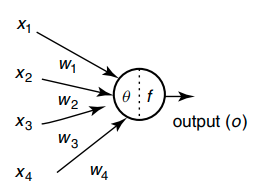
\includegraphics[width=0.5\textwidth]{imagenes/neuron}
        \end{center}
        \caption[Neurona Artificial]{}
    \end{figure}

Cada \textbf{neurona} realiza una operación simple: recibe varias entradas, las
pondera por medio de \textbf{pesos} $w_{i}$, suma estos valores junto con un \textbf{sesgo} $b$, y aplica una función
de activación.
La salida de la neurona se expresa como:

$z =w_{1}x_{1} + w_{2}x_{2} + \dots + w_{n}x_{n} + b_{z} = w_{1}x_{1} + w_{2}x_{2} + \dots + w_{n}x_{n} + b$

Luego, el valor $z$ pasa por una función de activación, que introduce la no linealidad en el sistema, permitiendo que
las redes neuronales modelen relaciones complejas.
    \item \textbf{Capas de la Red}:
    \begin{figure}[htp] \label{fig:capas-red-neuronal}
        \begin{center}
            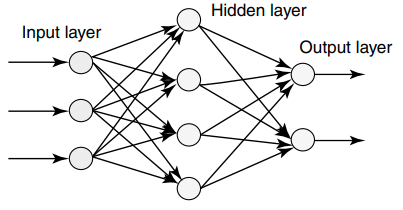
\includegraphics[width=0.5\textwidth]{imagenes/capas_red_neuronal}
        \end{center}
        \caption[Capas de la Red Neuonial Artificial]{}
    \end{figure}
\begin{itemize}
    \item \textbf{Capa de entrada}: Es la primera capa de la red neuronal, que recibe los datos crudos (por ejemplo,
píxeles de una imagen).
    \item \textbf{Capas ocultas}: Estas capas intermedias entre la entrada y la salida aprenden representaciones
abstractas de los datos.
En una red profunda, hay múltiples capas ocultas, lo que permite la \textbf{transformación jerárquica} de los datos.
    \item \textbf{Capa de salida}: Produce la predicción final, que puede ser una clase (en problemas de clasificación)
o un valor numérico (en problemas de regresión).
\end{itemize}
    \item \textbf{Pesos y Bias}: Los \textbf{pesos} son parámetros ajustables que determinan la importancia de cada
entrada en la neurona.
El \textbf{bias} es otro parámetro que se suma al valor ponderado para desplazar la activación de la neurona y permitir
que el modelo ajuste mejor los datos.

    \item \textbf{Funciones de Activación}: Las funciones de activación son fundamentales para que las redes neuronales
puedan aprender relaciones no lineales.
Entre las más comunes se encuentran:
\begin{itemize}
    \item \textbf{ReLU(Rectified Linear Unit)}: $ReLU(x)=\max(0,x)$, que activa solo valores positivos.
    \item \textbf{Sigmoide}: Que transforma los valores en un rango entre 0 y 1.
    \item \textbf{Tanh (Tangente hiperbólica)}: Transforma los valores en un rango entre -1 y 1.
\end{itemize}
\end{enumerate}

El uso de \textbf{backpropagation} o retropropagación permite ajustar los pesos y biases durante el entrenamiento
mediante un algoritmo de optimización, como el descenso de gradiente.
De esta manera, la red aprende minimizando la diferencia entre sus predicciones y las respuestas correctas.
\section{Redes Neuronales Convolucionales}\label{sec:redes-neuronales-convolucionales}
Las \textbf{Redes Neuronales Convolucionales} (Convolutional Neural Networks, CNNs) son una clase de redes neuronales
profundas especialmente efectivas para el procesamiento de datos que tienen una estructura de tipo rejilla, como las
imágenes.
Fueron inspiradas por el sistema visual de los mamíferos, donde diferentes capas de neuronas responden a estímulos
visuales de manera jerárquica. \\[2pt]

Las CNNs son ampliamente utilizadas en tareas de \textbf{visión por computador}, como el reconocimiento de imágenes, la
segmentación de objetos y la clasificación de imágenes.
Lo que diferencia a las CNNs de las redes neuronales tradicionales es su capacidad para detectar
\textbf{patrones espaciales} como bordes, texturas, y formas, sin necesidad de un procesamiento manual de las
características.


\subsection{Componentes principales de una CNN}\label{subsec:componentes-principales-de-una-cnn}
\begin{figure}[htp] \label{fig:convolution-layer}
    \begin{center}
        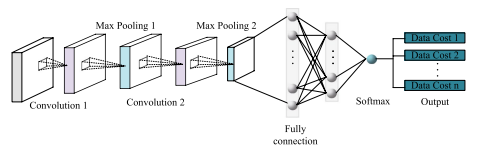
\includegraphics[width=1\textwidth]{imagenes/convolution_layer}
    \end{center}
    \caption[Puntos globales y locales]{En esta imagen extraída de
    \cite{A review of convolutional neural networks in computer vision} puede observarse de la estructura de una red
    neuronale convolucional. Junto a sus capas convolucionales. }
\end{figure}

\begin{enumerate}
    \item \textbf{Capas Convolucionales}: Estas capas aplican \textbf{filtros o kernels} sobre las imágenes de entrada
para detectar características locales, como bordes, esquinas o texturas.
Un filtro convolucional es una pequeña matriz que se mueve a lo largo de la imagen, calculando productos escalares en
cada posición para producir un mapa de características.

Las convoluciones son útiles porque explotan la \textbf{localidad de las características}, es decir, las relaciones
espaciales entre píxeles cercanos.
Además, la cantidad de parámetros se reduce drásticamente en comparación con las capas densas, ya que el filtro se
comparte a lo largo de la imagen.
    \item \textbf{Pooling (Submuestreo o Agrupamiento)}: Las capas de pooling reducen la dimensionalidad de las
características extraídas por las capas convolucionales, lo que hace que las representaciones sean más manejables y
robustas frente a pequeños cambios o desplazamientos en la imagen.

El max-pooling es la técnica de pooling más común, donde se toma el valor máximo dentro de una ventana de píxeles,
reduciendo el tamaño de la imagen, pero reteniendo las características más importantes.
    \item \textbf{Capas Densas}: Después de varias capas convolucionales y de pooling, se agregan una o más
\textbf{capas densas} (fully connected) para realizar la clasificación o predicción final.
Estas capas toman todas las características aprendidas en las capas convolucionales y las combinan para generar una
decisión final.
    \item \textbf{Batch Normalization}: Esta técnica se utiliza para \textbf{normalizar} las salidas de las capas
intermedias de una red neuronal.
Batch Normalization ayuda a \textbf{acelerar el entrenamiento} y a hacer que la red sea más estable, al reducir el
\textbf{desplazamiento covariante} (cambios en las distribuciones de las entradas de las capas intermedias a lo largo
del entrenamiento).
Esto se logra al normalizar las entradas de cada capa convolucional o densa antes de aplicar la activación, ajustando
su media y varianza.

    \item \textbf{Dropout}: El Dropout es una técnica de \textbf{regularización} que se utiliza para prevenir el
\textbf{sobreajuste} (overfitting) durante el entrenamiento de una red neuronal.
Durante cada iteración del entrenamiento, Dropout \textbf{desactiva aleatoriamente} un porcentaje de las neuronas, lo
que obliga a la red a no depender excesivamente de ciertas neuronas y a ser más robusta.
Esta técnica mejora la generalización de la red, lo que la hace funcionar mejor en datos no vistos.

\end{enumerate}

\subsection{Funcionamiento General de una CNN}\label{subsec:funcionamiento-general-de-una-cnn}
Al pasar una imagen a través de varias capas convolucionales, la red aprende a identificar características simples como
líneas y bordes.
Conforme avanza a capas más profundas, las características se vuelven más abstractas, capturando patrones más complejos
como formas, texturas y, finalmente, estructuras completas como objetos. \\[6pt]

Por ejemplo, en una red entrenada para reconocer caras, las primeras capas pueden detectar bordes o contornos, las
capas intermedias pueden aprender a reconocer ojos, nariz o boca, y las últimas capas pueden identificar una cara
completa.

\subsection{Aplicaciones de las CNN}\label{subsec:aplicaciones-de-las-cnn}
\begin{itemize}
    \item \textbf{Clasificación de imágenes}: Etiquetar imágenes en distintas categorías, como identificar animales o
vehículos.
    \item \textbf{Detección de objetos}: Identificar y localizar objetos en imágenes.
    \item \textbf{Reconocimiento facial}: Utilizado en sistemas de seguridad, como el desbloqueo de teléfonos móviles.
\end{itemize}

Las CNN son fundamentales en muchas aplicaciones modernas debido a su capacidad para procesar y entender datos visuales
de manera eficiente y automática.

\section{Datasets}\label{sec:datasets}
En el aprendizaje profundo, los datasets son colecciones de datos etiquetados o no etiquetados que se utilizan para
entrenar modelos.
Estos conjuntos de datos suelen contener ejemplos organizados que representan la entrada para el modelo, y en muchos
casos, también las etiquetas correspondientes que indican la salida deseada.
Los datasets varían en tamaño, calidad y tipo, dependiendo de la tarea a resolver, como la clasificación de imágenes,
el reconocimiento de patrones o la predicción de series temporales.

\subsection{Rock, Paper, Scissors (Piedra, Papel, Tijera)}\label{subsec:rock-paper-scissors}
\textbf{Rock, Paper, Scissors}~\cite{Rock Paper Scissors Dataset} fue creado originalmente por Laurence Moroney y se
utiliza para clasificar imágenes de las manos representando los gestos de `piedra', `papel' y `tijeras'.
El conjunto de datos contiene alrededor de 2,500 imágenes distribuidas en tres categorías: piedra, papel y tijeras.
Las imágenes están en color y tienen un tamaño de 300x300 píxeles. \\[6pt]

En este trabajo, se ha utilizado el dataset de \textbf{Rock, Paper, Scissors} para evaluar el rendimiento del modelo en
un problema de clasificación de imágenes más variado y natural, que involucra múltiples clases.
Además, permite explorar la eficacia de los algoritmos meméticos en un entorno más cercano al reconocimiento de
objetos, lo que añade mayor complejidad al problema.

\subsection{MNIST (Modified National Institute of Standards and Technology)}\label{subsec:mnist}
\textbf{MNIST}~\cite{MNIST Dataset} es uno de los datasets más utilizados en el campo del aprendizaje automático y el
aprendizaje profundo.
Contiene 70,000 imágenes de dígitos escritos a mano (60,000 para el conjunto de entrenamiento y 10,000 para el de
prueba).
Las imágenes son en escala de grises y tienen un tamaño de 28x28 píxeles, con cada píxel representando una intensidad
de color entre 0 (negro) y 255 (blanco).

Este dataset se utiliza comúnmente como \textbf{benchmark} para evaluar modelos de clasificación de imágenes,
particularmente en arquitecturas convolucionales.

La simplicidad de \textbf{MNIST} lo hace ideal para probar modelos de redes neuronales convolucionales, ya que ofrece un
equilibrio entre un problema fácil de entender, pero con suficiente complejidad para que los modelos más avanzados
demuestren mejoras.

\subsection{Comparación con otros datasets}\label{subsec:comparacion-con-otros-datasets}
La selección de estos dos datasets responde a la necesidad de evaluar los algoritmos meméticos en distintos niveles de
complejidad.
\textbf{MNIST}, con imágenes en escala de grises de bajo nivel de complejidad, proporciona una referencia clara y
estandarizada para comparar el rendimiento y la reducción de datos.
Por otro lado, el dataset de \textbf{Rock, Paper, Scissors} introduce más desafíos visuales y complejidades,
permitiendo analizar cómo los algoritmos meméticos se comportan en escenarios más complejos que podrían ser
representativos de aplicaciones más reales en visión por computadora.

\section{Modelos}\label{sec:modelos}
En el ámbito del aprendizaje profundo, existen diversas arquitecturas de redes neuronales convolucionales que han
demostrado un rendimiento excepcional en diversas tareas de visión por computadora.
Estas arquitecturas están diseñadas para abordar problemas complejos y variados, desde la clasificación de imágenes
hasta la detección de objetos y el segmentado de imágenes. \\[6pt]

A continuación, se explorarán algunas de estas arquitecturas que representan avances significativos en la eficiencia y
efectividad del aprendizaje profundo.

\subsection{ResNet50}\label{subsec:resnet50}
\textbf{ResNet50}~\cite{resnet} es una arquitectura de red neuronal convolucional introducida por Kaiming He et al. en 2015.
La principal innovación de ResNet es la introducción de \textbf{bloques de residualidad}, que permiten la construcción
de redes extremadamente profundas sin el problema de la degradación del rendimiento. \\[6pt]

La idea básica de los bloques residuales es permitir que la red aprenda funciones de identidad, facilitando así la
propagación de la información y el gradiente a través de la red.
En términos prácticos, esto se traduce en un rendimiento mejorado en tareas de clasificación de imágenes, donde
ResNet50 ha logrado resultados sobresalientes en competiciones como ImageNet. \\[6pt]

ResNet50 está compuesta por 50 capas, de las cuales 49 son capas convolucionales y una es una capa totalmente conectada.
La arquitectura incluye capas de normalización y activación (ReLU), así como una estructura que permite saltos de
conexión, lo que significa que la entrada de una capa se suma a la salida de una capa posterior.

\subsection{MobileNetV2}\label{subsec:mobilenet}
\textbf{MobileNet}~\cite{} es una arquitectura de red neuronal diseñada específicamente para aplicaciones móviles y de visión
por computadora en dispositivos con recursos limitados.
Introducida por Andrew G. Howard et al.\ en 2017, MobileNet se basa en el principio de
\textbf{convoluciones separables en profundidad} (depthwise separable convolutions), que dividen el proceso de
convolución en dos pasos: primero, se aplica una convolución a cada canal de la entrada (depthwise), y luego, se
combinan los resultados con una convolución 1x1 (pointwise). \\[6pt]

Esta técnica reduce significativamente el número de parámetros y el costo computacional, lo que permite ejecutar
modelos de visión por computadora en dispositivos móviles sin sacrificar drásticamente la precisión.

\subsubsection{MobileNetV2}\label{subsubsec:mobilenetv2}
\textbf{MobileNetV2}~\cite{}, introducido por Sandler et al.\ en 2018, mejora la arquitectura de MobileNet original al
incorporar varias innovaciones.
La principal contribución de MobileNetV2 es la introducción de los bloques de \textbf{residualidad invertida} (inverted
residuals), que permiten que la red mantenga una mayor capacidad de representación y flujo de información a través de
las capas. \\[6pt]

Además, MobileNetV2 utiliza una función de activación llamada \textbf{linear bottleneck}, que ayuda a preservar la
información durante la propagación a través de las capas, lo que mejora aún más el rendimiento del modelo en tareas de
clasificación y detección.
Esta arquitectura se optimiza para ser altamente eficiente, permitiendo que sea utilizada en aplicaciones de tiempo
real en dispositivos con limitaciones de hardware. \\[6pt]

MobileNetV2 ha demostrado ser una opción popular para aplicaciones en dispositivos móviles y sistemas embebidos,
ofreciendo un buen equilibrio entre precisión y eficiencia computacional.

\chapter{Repaso Bibliográfico}\label{ch:repaso_bibliografico}
%Repaso Bibliográfico: Revisión de trabajos previos relevantes en el área.
% !TeX root = ../proyecto.tex

\chapter{Descripción de los Algoritmos}\label{ch:descripcion-algoritmos}
En este capítulo se describen los diferentes algoritmos utilizados en el desarrollo de este trabajo.
Todos ellos tienen como objetivo principal reducir el tamaño del conjunto de datos de entrenamiento utilizado en los
modelos de aprendizaje profundo, con el fin de optimizar el rendimiento y reducir el costo computacional.
El enfoque adoptado en este trabajo es la aplicación de algoritmos meméticos, los cuales combinan principios de
algoritmos genéticos con estrategias de búsqueda local.


A continuación, se detallan los algoritmos principales implementados en este proyecto: el \textbf{algoritmo aleatorio},
el \textbf{algoritmo de búsqueda local} y el \textbf{algoritmo genético}

\section{Algoritmo Aleatorio}\label{sec:algoritmo-aleatorio}
%Algoritmos Meméticos: Detalla qué son y cómo se aplican a la reducción de datos.
El \textbf{algoritmo aleatorio} sirve como referencia básica para medir la efectividad de los algoritmos más avanzados.
Este enfoque selecciona subconjuntos de datos de manera completamente aleatoria, sin aplicar ningún tipo de estrategia
de optimización.

\subsection{Descripción}\label{subsec:descripcion}
El algoritmo comienza tomando el conjunto de datos completo y seleccionando una fracción de los ejemplos de
entrenamiento de forma aleatoria.
Esta selección se realiza sin ningún criterio basado en la relevancia de los datos, lo que implica que el conjunto de
entrenamiento resultante puede no ser representativo o puede contener redundancias innecesarias.

\subsection{Aplicación en la reducción de datos}\label{subsec:aplicacion-en-la-reduccion-de-datos}
A pesar de su simplicidad, el \textbf{algoritmo aleatorio} puede ser útil como método de comparación.
En muchos casos, los algoritmos más complejos deben demostrar que pueden superar este enfoque básico en términos de
precisión y eficiencia.
Al seleccionar datos de manera aleatoria, este método a menudo produce conjuntos de entrenamiento subóptimos, lo que
resulta en modelos menos precisos o con mayor varianza.

\subsection{Resultados esperados}\label{subsec:resultados-esperados}
Debido a la naturaleza aleatoria del algoritmo, los resultados son altamente variables.
Es probable que en muchas ejecuciones el rendimiento del modelo entrenado sea inferior al obtenido con métodos más
estructurados.
Este algoritmo proporciona una línea base importante para evaluar la efectividad de los algoritmos más avanzados.


\section{Algoritmo Búsqueda Local}\label{sec:algoritmo-busqueda-local}
El \textbf{algoritmo de búsqueda local} es una técnica más sofisticada que explora el espacio de soluciones de manera
más estructurada, buscando mejorar progresivamente una solución inicial.

\subsection{Descripción}\label{subsec:descripcion2}
La búsqueda local se basa en la idea de comenzar con una solución inicial (un subconjunto de datos) y realizar pequeños
cambios o `movimientos' en esa solución para explorar otras soluciones cercanas.
En este contexto, cada solución es un subconjunto de datos.
El algoritmo evalúa diferentes subconjuntos de datos probando si estos mejoran el rendimiento del modelo de aprendizaje
profundo al entrenarlo con ellos.


El proceso básico de la búsqueda local es el siguiente:
\begin{enumerate}
      \item Se genera una solución inicial, por ejemplo, seleccionando un subconjunto de datos aleatoriamente.
      \item Se realizan cambios locales en la solución, como añadir o eliminar ejemplos del conjunto de datos.
      \item Se evalúa la nueva solución según el rendimiento del modelo de aprendizaje profundo.
      \item Si la nueva solución es mejor, se reemplaza la solución actual por esta.
      \item El proceso se repite hasta que no se observan mejoras significativas o hasta que se alcanza un número
      \item predefinido de iteraciones.
\end{enumerate}

\subsection{Aplicación en la reducción de datos}\label{subsec:aplicacion-en-la-reduccion-de-datos2}
En el contexto de la reducción de datos, el objetivo de la búsqueda local es identificar un subconjunto más pequeño de
ejemplos que sea suficiente para entrenar el modelo con un rendimiento similar al obtenido con el conjunto de datos
completo.
La búsqueda local explora el espacio de posibles subconjuntos, eliminando ejemplos redundantes o irrelevantes, y
conservando solo aquellos que son cruciales para el rendimiento del modelo.

\subsection{Ventajas y limitaciones}\label{subsec:ventajas-y-limitaciones}
\textbf{Ventajas}: Este enfoque permite una exploración más exhaustiva del espacio de soluciones que un algoritmo
aleatorio.
Al hacer pequeños ajustes en cada iteración, el algoritmo puede encontrar mejores soluciones de manera eficiente.
\textbf{Limitaciones}: Sin embargo, la búsqueda local puede quedarse atrapada en \textbf{óptimos locales}, es decir,
soluciones que parecen buenas en comparación con las cercanas, pero que no son globalmente óptimas.

\section{Algoritmos Genéticos}\label{sec:algoritmos-geneticos}
Los \textbf{algoritmos genéticos} son algoritmos de búsqueda inspirados en los principios de la evolución natural.
En este trabajo, se aplican con el objetivo de encontrar subconjuntos óptimos de datos de entrenamiento, reduciendo el
tamaño del conjunto mientras se mantiene o mejora el rendimiento del modelo de aprendizaje profundo.

\subsection{Descripción}\label{subsec:descripcion3}
El funcionamiento de los algoritmos genéticos se basa en los conceptos de \textbf{selección natural},
\textbf{cruzamiento} y \textbf{mutación}.
El proceso se puede resumir en los siguientes pasos:
\begin{enumerate}
      \item \textbf{Inicialización}: Se genera una población inicial de posibles soluciones, cada una de ellas
            representando un subconjunto del conjunto de datos.
      \item \textbf{Evaluación}: Cada subconjunto de datos (o `individuo') es evaluado entrenando el modelo con ese
            subconjunto y midiendo su rendimiento.
      \item \textbf{Selección}: Se seleccionan los mejores individuos de la población basándose en su rendimiento.
            Los mejores individuos tienen más probabilidades de ser seleccionados para la siguiente generación.
      \item \textbf{Cruzamiento}: Se combinan pares de individuos seleccionados para crear nuevos subconjuntos.
            Esto se realiza intercambiando ejemplos entre los subconjuntos.
      \item \textbf{Mutación}: Con una pequeña probabilidad, se realizan cambios aleatorios en algunos individuos, como
            añadir o eliminar ejemplos del subconjunto.
      \item \textbf{Iteración}: El proceso de evaluación, selección, cruzamiento y mutación se repite durante varias
            generaciones, con la esperanza de que cada generación produzca soluciones mejores que la anterior.
\end{enumerate}

\subsection{Aplicación en la reducción de datos}\label{subsec:aplicacion-en-la-reduccion-de-datos3}
Los \textbf{algoritmos genéticos} son especialmente adecuados para la reducción de datos porque permiten explorar un
espacio de soluciones muy amplio de manera eficiente.
La combinación de individuos y la introducción de mutaciones aleatorias permiten al algoritmo escapar de los óptimos
locales, un problema común en la búsqueda local.

El uso de algoritmos genéticos para reducir datos en este contexto implica encontrar subconjuntos de entrenamiento que
proporcionen un buen equilibrio entre tamaño y rendimiento.
Esto se logra al evaluar diferentes subconjuntos y mejorar las soluciones generación tras generación.

\subsection{Ventajas y limitaciones}\label{subsec:ventajas-y-limitaciones2}
\textbf{Ventajas}: Los algoritmos genéticos son efectivos para explorar grandes espacios de soluciones y tienen una
gran capacidad para evitar quedar atrapados en óptimos locales.
Son especialmente útiles en problemas donde la solución óptima no es evidente desde el principio.


\textbf{Limitaciones}: Estos algoritmos pueden ser costosos computacionalmente, ya que requieren evaluar muchas
soluciones a lo largo de múltiples generaciones.
Además, su convergencia a veces puede ser lenta, dependiendo del tamaño del espacio de búsqueda y de los
parámetros del algoritmo (tamaño de la población, tasa de mutación, etc.).

\subsection{Versiones}\label{subsec:versiones}

% !TeX root = ../proyecto.tex

\chapter{Implementación}\label{ch:implementacion}
En este capítulo se presenta en detalle la arquitectura técnica del sistema implementado, incluyendo los componentes y
módulos principales, las herramientas específicas empleadas en la construcción del sistema, y los elementos clave para
optimizar el rendimiento de los algoritmos y su evaluación.


\section{Descripción del Sistema}\label{sec:descripcion-del-sistema}
%Descripción del Sistema: Detalla la arquitectura del sistema que estás implementando.
La estructura del proyecto se organizó modularmente para facilitar el acceso, el mantenimiento y la extensibilidad del código fuente.
La organización de carpetas es la siguiente:
\begin{itemize}
      \item \texttt{data} -- Conjunto de datos utilizados en los experimentos.
      \item \texttt{docs} -- Documentación del proyecto en latex.
            \begin{itemize}
                  \item \texttt{bibliografia} -- Archivos relacionados con las referencias bibliográficas.
                  \item \texttt{capitulos} -- Archivos individuales para cada capítulo del documento.
                  \item \texttt{config} -- Archivos de configuraciones de la documentación LaTeX.
                  \item \texttt{imagenes} -- Imágenes utilizadas en la documentación.
                  \item \texttt{out} -- Archivos generados por el compilador de LaTeX.
                  \item \texttt{portada} -- Archivo portada del documento.
                  \item \texttt{prefacio} -- Archivo prefacio del documento.
                  \item \texttt{proyecto.tex} -- Archivo principal de LaTeX que compila el documento.
            \end{itemize}
      \item \texttt{img} -- Imágenes generadas automáticamente durante los experimentos.
      \item \texttt{LICENSE} -- Términos de distribución del proyecto.
      \item \texttt{logs} -- Registros de las ejecuciones, incluyendo tiempos de inicio, fin y resultados intermedios de los algoritmos.
      \item \texttt{README.md} -- Descripción general.
      \item \texttt{requirements.txt} -- Dependencias del proyecto.
      \item \texttt{results} -- Resultados de los experimentos.
            \begin{itemize}
                  \item \texttt{csvs} -- Resultados de las ejecuciones guardados en tablas.
                  \item \texttt{salidas} -- Salidas en bruto de consola.
            \end{itemize}
      \item \texttt{scripts} -- Scripts de ejecución automática, comparación de experimentos y generación de gráficos finales.
      \item \texttt{src} -- Código fuente principal del proyecto.
            \begin{itemize}
                  \item \texttt{algorithms} -- Implementaciones de los algoritmos.
                  \item \texttt{main.py} -- Módulo principal de ejecución individual.
            \end{itemize}
      \item \texttt{tmp} -- Ficheros temporales generados durante la ejecución.
      \item \texttt{utils} -- Módulos de apoyo, como clases auxiliares, generación de gráficos y funciones utilitarias.
\end{itemize}

El código completo del proyecto, incluyendo los scripts, algoritmos, documentación y resultados,
se encuentra disponible en el repositorio público de GitHub: \url{https://github.com/JoseRuizLopez/TFG}.


\section{Herramientas y Lenguajes de Programación}\label{sec:herramientas-y-lenguajes-de-programacion}
%Herramientas y Lenguajes de Programación: Lista las herramientas y tecnologías que usarás.
El desarrollo del proyecto se ha llevado a cabo utilizando \textbf{Python 3.10}~\cite{vanderplasPythonDataScience2016} como
lenguaje principal, debido a su versatilidad y amplia adopción en el campo del \textbf{aprendizaje profundo} y la
\textbf{manipulación de datos}.
Python es conocido por su facilidad de uso, extensibilidad y la gran cantidad de bibliotecas disponibles para el
procesamiento de datos y la implementación de modelos de \textbf{machine learning}.


Las principales bibliotecas empleadas durante el desarrollo son las siguientes:
\begin{itemize}
      \item \textbf{PyTorch 2.3.1}~\cite{ketkarIntroductionPyTorch2021, TorchcudaPyTorch24}: Para la construcción,
            entrenamiento y optimización de modelos de aprendizaje profundo.
            PyTorch fue elegido por su flexibilidad y capacidad para ejecutarse eficientemente en GPU\@.
      \item \textbf{Scikit-learn 1.5.2}~\cite{vanderplasPythonDataScience2016}: Para la evaluación de los modelos se utilizaron
            métricas estándar~\cite{kramerScikitLearn2016}.
            Su API permite una integración fluida con PyTorch y otros módulos.
      \item \textbf{Numpy 2.0.0}~\cite{NumPyV20Manual}: Para operaciones matemáticas y manipulación de matrices,
            siendo una herramienta esencial en el procesamiento de datos.
      \item \textbf{Polars 1.9.0}~\cite{PolarsPythonAPI}: Biblioteca para manejar DataFrames de gran tamaño,
            elegida por su rendimiento superior en comparación con Pandas.
      \item \textbf{Matplotlib 3.9.2}~\cite{Matplotlib393Documentation}: Biblioteca utilizada para la generación y
            visualización de gráficas.
      \item \textbf{Seaborn 0.13.2}~\cite{Seaborn0132Documentation}: Estilización avanzada de gráficos estadísticos.
      \item \textbf{Openpyxl 3.1.5}~\cite{Openpyxl313Documentation}: Generación automática de archivos Excel a partir de resultados experimentales.
\end{itemize}

Cada una de estas herramientas fue seleccionada por su robustez y su idoneidad para cumplir con los requisitos
específicos del proyecto, facilitando tanto la implementación de los algoritmos meméticos como la reducción y el
análisis de los datos utilizados en los modelos de aprendizaje profundo.

\section{Gestión de Dependencias}\label{sec:gestion-de-dependencias}
Para garantizar que el proyecto se ejecute correctamente y todas las bibliotecas necesarias estén disponibles, se ha
utilizado un archivo \texttt{requirements.txt}.
Este archivo contiene una lista de todas las bibliotecas y sus versiones específicas que el proyecto requiere.


Para el \textbf{desarrollo local}, se ha optado por crear un entorno virtual utilizando
\texttt{venv}~\cite{CreationVirtualEnvironments}.
Esta práctica permite aislar las dependencias del proyecto de otros proyectos en la máquina, evitando conflictos entre
versiones de bibliotecas.


Para la \textbf{implementación en el servidor}, se ha utilizado \texttt{conda}~\cite{CondaDocumentation} como gestor
de paquetes y entornos.
Conda facilita la gestión de entornos y la instalación de bibliotecas, especialmente en configuraciones más complejas.



Esto facilita la reproducibilidad del proyecto y minimiza posibles conflictos de versión, lo que es fundamental para
mantener la integridad del código y el rendimiento de las aplicaciones.

\section{Arquitectura de la Implementación}\label{sec:arquitectura-de-la-implementacion}
La arquitectura de la implementación desarrollada para este trabajo está diseñada con un enfoque modular y escalable,
que permite gestionar de forma eficiente las distintas fases del proceso de selección de instancias y evaluación de modelos.
El sistema se compone de varios módulos interrelacionados que se encargan de la generación de subconjuntos,
la ejecución de los algoritmos evolutivos y meméticos, la evaluación de las soluciones mediante modelos preentrenados, y la visualización y almacenamiento de resultados.
Esta estructura facilita la incorporación de nuevos algoritmos o mejoras en los ya existentes, garantizando una mayor flexibilidad y mantenimiento del código.

\subsection{Esquema General de Funcionamiento de los Algoritmos}\label{subsec:esquema-algoritmos}
El funcionamiento general de los algoritmos implementados en este trabajo sigue un flujo estructurado y modular que permite una ejecución ordenada de todas las etapas del proceso.
La Figura~\ref{fig:esquema-flujo-algoritmos} muestra el esquema general de funcionamiento, desde la configuración inicial hasta la evaluación final de resultados.

\begin{figure}[htp]
      \centering
      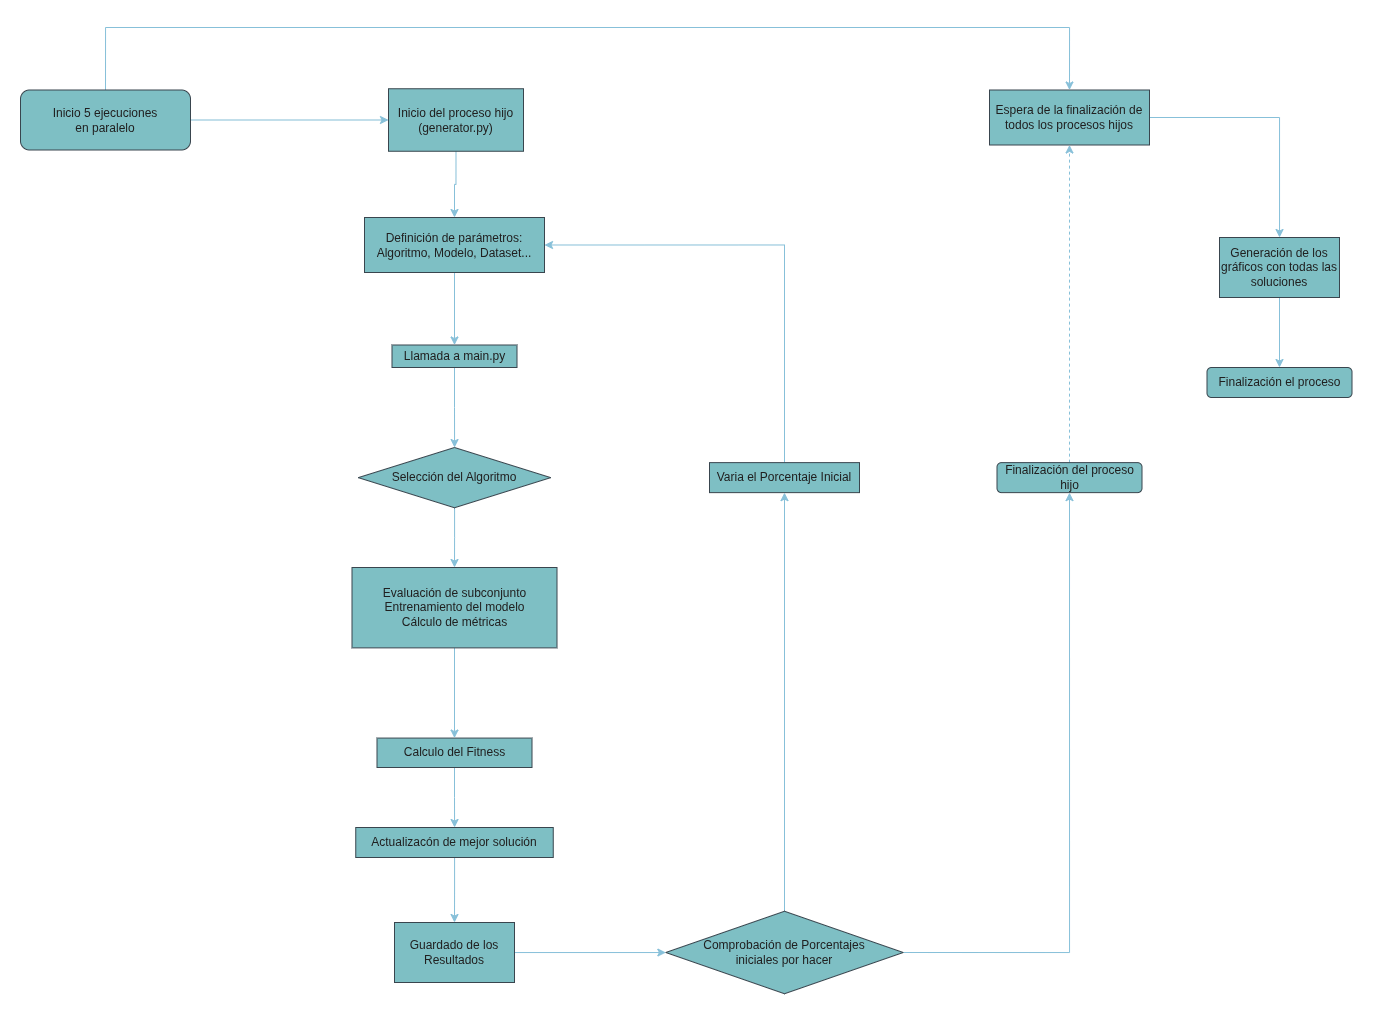
\includegraphics[width=0.95\textwidth]{imagenes/flujo2.drawio}
      \caption{Esquema general del flujo de ejecución de los algoritmos y evaluación de subconjuntos.}
      \label{fig:esquema-flujo-algoritmos}
\end{figure}

El proceso se organiza en los siguientes pasos principales:

\begin{enumerate}
      \item \textbf{Ejecución del script de paralelización:} Se inicia el script que permite ejecutar múltiples experimentos de manera paralela,
            facilitando la obteción de resultados de diferentes semillas.
      \item \textbf{Configuración inicial:} Se define el algoritmo, el modelo y el dataset a utilizar, a través de los parámetros en \texttt{generator.py}.
      \item \textbf{Ejecución del núcleo principal:} El script \texttt{main.py} se encarga de orquestar la ejecución,
            llamando a las funciones específicas según el algoritmo seleccionado.
      \item \textbf{Generación y evaluación de subconjuntos:} Cada algoritmo genera subconjuntos de datos de entrenamiento a partir del conjunto original.
      \item \textbf{Entrenamiento del modelo:} Se realiza el entrenamiento del modelo utilizando los subconjuntos generados,
            aplicando técnicas de \textit{transfer learning} con modelos preentrenados.
      \item \textbf{Almacenamiento de resultados:} Cada evaluación almacena los resultados obtenidos (métricas y composición del subconjunto) y,
            tras finalizar la ejecución, se generan gráficos como boxplots y visualizaciones que permiten analizar el rendimiento de cada enfoque.
\end{enumerate}

\subsection{Configuración de Modelos Preentrenados}\label{subsec:configuracion-modelos-preentrenados}
En este trabajo, se han utilizado modelos convolucionales preentrenados como base para la tarea de clasificación de imágenes.
Concretamente, se han empleado las arquitecturas \textbf{ResNet50} y \textbf{MobileNetV2},
cargadas con pesos preentrenados sobre \texttt{ImageNet} o \texttt{CIFAR10}, según el dataset utilizado en cada experimento.

Para adaptar estos modelos a la tarea específica de clasificación de subconjuntos de datos,
se ha seguido una estrategia de \textit{transfer learning} que permite reducir significativamente el coste computacional del entrenamiento.
Esta estrategia consiste en congelar todas las capas del modelo, excepto la última,
de manera que las representaciones aprendidas en la etapa preentrenada puedan ser reutilizadas como extractores de características generales.

Específicamente, la \textbf{última capa} de cada modelo preentrenado (la capa densa o \textit{fully connected})
ha sido reemplazada por una nueva capa completamente conectada (\texttt{Linear}) adaptada al número de clases del dataset en uso.
Esta capa es la única que se entrena durante la fase de evaluación de cada subconjunto generado por los algoritmos,
permitiendo obtener métricas como \textit{accuracy}, \textit{precision}, \textit{recall} y \textit{F1-score} de forma eficiente.

El uso de pesos preentrenados y la congelación de capas proporcionan varias ventajas:
\begin{itemize}
      \item Reducción del tiempo de entrenamiento en cada evaluación.
      \item Aprovechamiento de representaciones genéricas previamente aprendidas, lo que mejora la generalización.
      \item Adaptabilidad de los modelos a distintos datasets y tareas, modificando únicamente la capa final.
\end{itemize}

Este enfoque se implementa mediante las herramientas de PyTorch,
congelando explícitamente los gradientes de todas las capas del modelo y definiendo la nueva capa final con el número adecuado de salidas para cada problema de clasificación.

\subsection{Módulo de Algoritmos}\label{subsec:modulo-de-algoritmos}
Ubicado en \texttt{src/algorithms/} este módulo contiene las implementaciones principales de los
algoritmos desarrollados en el proyecto.

Este módulo utiliza la arquitectura GPU para maximizar la velocidad de ejecución y está diseñado para ser escalable,
permitiendo la inclusión de nuevos operadores meméticos si es necesario.

\subsection{Núcleo de Ejecución}\label{subsec:nucleo-de-ejecucion}
El módulo \texttt{main.py} centraliza la ejecución de un experimento individual, inicializando configuraciones,
entrenando el modelo y generando gráficos.

Los pasos de la función principal de \texttt{main.py} es:
\begin{enumerate}
      \item \textbf{Establece Configuración Inicial}: Configura una semilla, elige el dataset y prepara un archivo de log.
      \item \textbf{Inicia el Proceso del Algoritmo}: Según el nombre del algoritmo (algoritmo) especificado, se llama a
            la función correspondiente (por ejemplo, genetic\_algorithm, memetic\_algorithm, etc.).
      \item \textbf{Almacena Resultados}: Una vez que el algoritmo termina, registra la duración, los resultados y la
            métrica final en un archivo.
      \item \textbf{Visualiza Resultados}: Si hay datos de fitness, genera una gráfica de la evolución del fitness a lo
            largo del proceso.
      \item \textbf{Genera un Resumen}: Calcula estadísticas adicionales (como porcentaje de clases seleccionadas en
            Paper, Rock y Scissors), y devuelve estos resultados junto con el historial de fitness.
\end{enumerate}

\subsection{Módulo de Utilidades}\label{subsec:modulo-de-utilidades}
La carpeta \texttt{utils/} contiene funciones auxiliares:
\begin{itemize}
      \item \textbf{utils\_plot.py}: Generación de gráficos.
      \item \textbf{classes.py}: Definición de enumeraciones para algoritmos, métricas, datasets y modelos.
      \item \textbf{utils.py}: Funciones de ayuda como el cálculo de métricas o la creación de diccionarios de selección de imágenes.
\end{itemize}

Estos módulos se encargan de generar gráficas comparativas entre distintos porcentajes o algoritmos y en
generar un CSV con los datos finales para ser analizados.

\subsection{Scripts de Ejecución en GPU}\label{subsec:scripts-de-ejecucion-en-gpu}
En scripts, se encuentran los programas necesarios para ejecutar los algoritmos en un servidor GPU, lo que permite
maximizar la eficiencia en el entrenamiento y la evaluación de modelos.
\begin{enumerate}
      \item \textbf{Configuración de GPU}: Los scripts están configurados para identificar y utilizar las GPU disponibles
            en el servidor, reduciendo los tiempos de entrenamiento de modelos.
      \item \textbf{Optimización de Ejecución}: Se implementaron configuraciones de batch size y técnicas de
            procesamiento paralelo en PyTorch, aprovechando la memoria y el poder de procesamiento de las GPU\@.
\end{enumerate}

Estos scripts están diseñados para ser ejecutados en un entorno de servidor, reduciendo los tiempos de prueba en el
entorno local y permitiendo un análisis iterativo más rápido.

\section{Consideraciones de Optimización}\label{sec:consideraciones-de-optimizacion}
Durante el desarrollo, se optimizaron varios aspectos para mejorar el rendimiento del sistema:

\begin{enumerate}
      \item \textbf{Aceleración en GPU}: Todas las operaciones de cálculo intensivo fueron migradas a la GPU mediante
            PyTorch.
      \item \textbf{Uso Eficiente de Memoria}: Con Polars y Numpy, se optimizó el manejo de grandes volúmenes de datos,
            utilizando tipos de datos específicos para reducir el uso de memoria.
      \item \textbf{Automatización de Evaluaciones}: Las pruebas de rendimiento se automatizaron, permitiendo una
            evaluación continua sin intervención manual.
      \item \textbf{Control de reproducibilidad}: Se fijaron semillas aleatorias en todas las librerías involucradas
            (random, numpy, torch, cuda) y se desactivaron los algoritmos no deterministas de cuDNN~\cite{CuBLASDeterministicAlgorithms}.
            Esta medida garantiza que las ejecuciones del sistema produzcan resultados consistentes entre sesiones,
            algo esencial en entornos de evaluación comparativa.
      \item \textbf{Diagnóstico automático de GPU}: Implementación de un script (cuda-diagnostic.py) que comprueba disponibilidad
            de CUDA y dispositivos antes de lanzar experimentos, garantizando un entorno correcto.
\end{enumerate}

Además, se implementó un mecanismo de \textbf{early stopping} basado en la ausencia de mejora del valor de fitness durante
un número determinado de evaluaciones consecutivas.
Aunque no se utiliza una pérdida de validación explícita como en enfoques tradicionales, este enfoque funcionalmente cumple el mismo propósito:
detener el algoritmo cuando se detecta estancamiento, reduciendo así el coste computacional innecesario~\cite{EarlyStoppingDiscussion2024}.


Gracias a estas optimizaciones, el sistema permite explorar un amplio abanico de configuraciones de manera eficiente, manteniendo la robustez y estabilidad de los resultados.

\section{Métricas de Evaluación}\label{sec:metricas-evaluacion}

Para evaluar el rendimiento de los modelos de clasificación utilizados en los experimentos,
se han empleado cuatro métricas estándar en el ámbito del aprendizaje automático: \textbf{accuracy}, \textbf{precisión}, \textbf{recall} y \textbf{F1-score}.
Dado que se trata de un problema multiclase, estas métricas se han calculado utilizando el promedio \textit{macro},
lo que implica computarlas individualmente para cada clase y luego obtener la media aritmética.

A continuación se describen y formalizan cada una de estas métricas:

\begin{itemize}
      \item \textbf{Accuracy} (exactitud): representa la proporción de predicciones correctas sobre el total de ejemplos.
            $$
                  Accuracy = \frac{TP + TN}{TP + TN + FP + FN}
            $$
            En el caso multiclase, se generaliza como:
            $$
                  \mathrm{Accuracy} = \frac{\text{Número de predicciones correctas}}{\text{Total de predicciones}}
            $$

      \item \textbf{Precisión}: mide cuántas de las instancias clasificadas como positivas fueron realmente positivas.
            En el caso multiclase (macro), se calcula como:
            $$
                  \text{Precisión}_{\text{macro}} = \frac{1}{C} \sum_{i=1}^{C} \frac{TP_i}{TP_i + FP_i}
            $$

      \item \textbf{Recall}: indica cuántas de las instancias realmente positivas fueron correctamente identificadas por el modelo:
            $$
                  \mathrm{Recall}_{\text{macro}} = \frac{1}{C} \sum_{i=1}^{C} \frac{TP_i}{TP_i + FN_i}
            $$

      \item \textbf{F1-score}: es la media armónica entre precisión y recall, útil cuando se desea un equilibrio entre ambas:
            $$
                  \mathrm{F1\text{-}score}_{\text{macro}} = \frac{1}{C} \sum_{i=1}^{C} \frac{2 \cdot \text{Precisión}_i \cdot \text{Recall}_i}{\text{Precisión}_i + \text{Recall}_i}
            $$
\end{itemize}

Donde:
\begin{itemize}
      \item $TP_i$: verdaderos positivos de la clase $i$
      \item $FP_i$: falsos positivos de la clase $i$
      \item $FN_i$: falsos negativos de la clase $i$
      \item $C$: número total de clases
\end{itemize}

Para facilitar la comprensión de estos conceptos, en la Figura~\ref{fig:matriz-confusion} se muestra una representación gráfica de una matriz de confusión.
\begin{figure}[H]
      \centering
      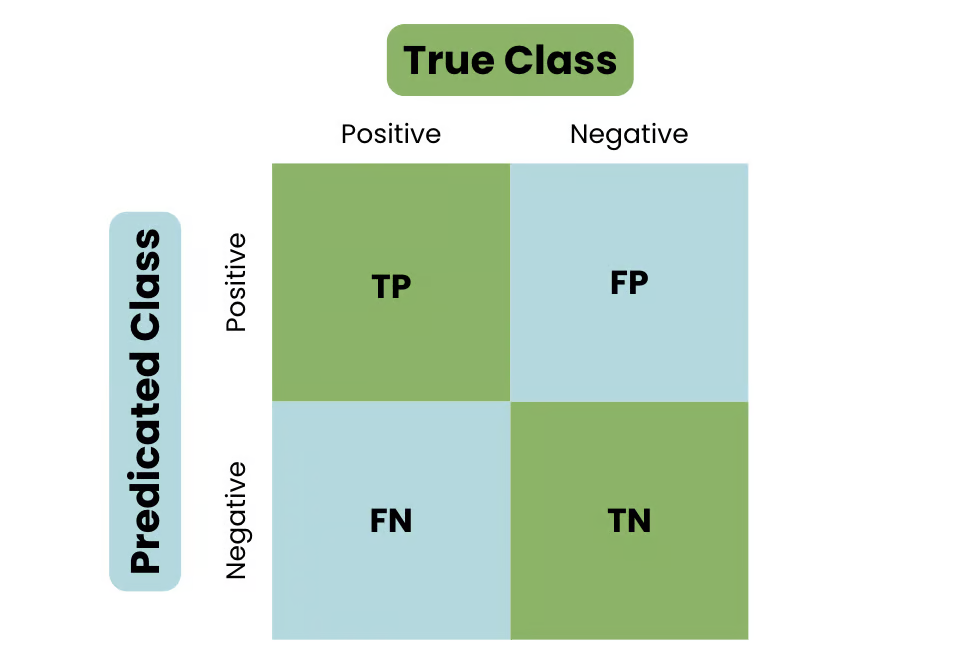
\includegraphics[width=0.5\textwidth]{imagenes/matriz-de-confusion.png}
      \caption{Representación gráfica de una matriz de confusión}
      \label{fig:matriz-confusion}
\end{figure}

Estas métricas fueron implementadas utilizando la librería \texttt{scikit-learn}, que permite su cálculo eficiente a partir de las
predicciones del modelo y las etiquetas reales del conjunto de validación.

% !TeX root = ../proyecto.tex

\chapter{Entorno de Pruebas}\label{ch:entorno_de_pruebas}
En este capítulo se describe el entorno experimental empleado para evaluar los algoritmos propuestos.
Se detallan los conjuntos de datos utilizados, el diseño de los experimentos, el procedimiento de ejecución y las métricas de evaluación.
Asimismo, se explica cómo se presentan y visualizan los resultados obtenidos.


\section{Datasets utilizados}\label{sec:datasets}
En el aprendizaje profundo, los datasets son colecciones de datos etiquetados o no etiquetados que se utilizan para
entrenar modelos.
Estos conjuntos de datos contienen ejemplos organizados que representan la entrada para el modelo y, en muchos casos,
también las etiquetas correspondientes que indican la salida deseada.
Los datasets varían en tamaño, calidad y tipo, dependiendo de la tarea a resolver, como la clasificación de imágenes,
el reconocimiento de patrones o la predicción de series temporales.


A continuación, se van a explicar cada uno de los Datasets que se han utilizado en el desarrollo del proyecto.

\subsection{Rock, Paper, Scissors (Piedra, Papel, Tijera)}\label{subsec:rock-paper-scissors}
\textbf{Rock, Paper, Scissors}~\cite{RockPaperScissors} es un conjunto de datos creado por Laurence Moroney
que se utiliza para la clasificación de imágenes de manos representando los gestos de `piedra', `papel' y `tijeras'.

\begin{figure}[htp]
    \centering
    \begin{subfigure}[t]{0.3\textwidth}
        \centering
        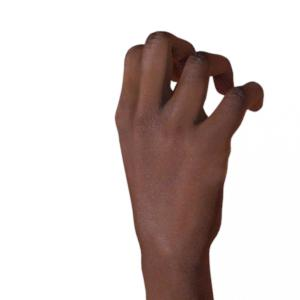
\includegraphics[width=\linewidth]{imagenes/dataset_examples/rock.jpg}
        \caption*{Rock}
    \end{subfigure}
    \begin{subfigure}[t]{0.3\textwidth}
        \centering
        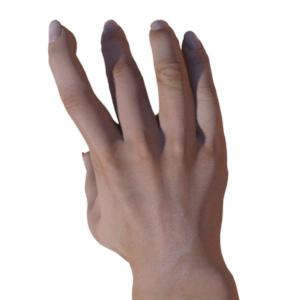
\includegraphics[width=\linewidth]{imagenes/dataset_examples/paper.jpg}
        \caption*{Paper}
    \end{subfigure}
    \begin{subfigure}[t]{0.3\textwidth}
        \centering
        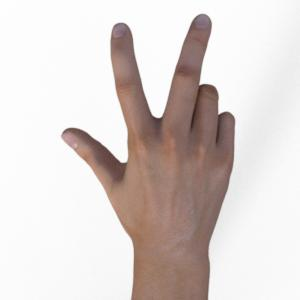
\includegraphics[width=\linewidth]{imagenes/dataset_examples/scissors.jpg}
        \caption*{Scissors}
    \end{subfigure}
    \caption{Ejemplos de imágenes del dataset Rock, Paper, Scissors}
    \label{fig:ejemplos-rps}
\end{figure}

En la figura~\ref{fig:ejemplos-rps} se han mostrado una imagen de cada una de las clases del dataset Rock, Paper, Scissors,
para que se pueda observar la similitud entre las distintas clases.

\subsubsection{Estructura del Dataset}
El conjunto de datos contiene aproximadamente 2,500 imágenes, distribuidas en tres categorías: piedra, papel y tijeras.
Las imágenes están en color y tienen un tamaño de 300x300 píxeles.

\begin{figure}[ht]
    \centering
    \begin{forest}mydirstyle
        [RPS
            [train
                    [rock
                            [image1.jpg]
                            [image2.jpg]
                            [\dots]
                    ]
                    [paper
                            [image1.jpg]
                            [image2.jpg]
                            [\dots]
                    ]
                    [scissors
                            [image1.jpg]
                            [image2.jpg]
                            [\dots]
                    ]
            ]
            [test (originalmente valid)
                [rock]
                    [paper]
                    [scissors]
            ]
            [valid (originalmente test)
                [rock]
                    [paper]
                    [scissors]
            ]
        ]
    \end{forest}
    \caption{Estructura de carpetas del dataset Rock, Paper, Scissors}
    \label{fig:estructura-rps}
\end{figure}


Como se puede observar en la Figura~\ref{fig:estructura-rps}, las imágenes están organizadas en directorios según su función en el entrenamiento
(entrenamiento, validación o prueba) y, dentro de cada partición, se dividen a su vez por clases del dataset.

\subsubsection{Formato de los Datos}
Las imágenes están en formato JPEG (\texttt{.jpg}).
Para su procesamiento, se han aplicado técnicas de preprocesamiento
adaptadas a los requerimientos del modelo.

\subsubsection{Uso del Dataset}
Este dataset se ha utilizado para evaluar el rendimiento del modelo en un problema de clasificación de imágenes con
múltiples clases, pero siendo un dataset sencillo y con un número de clases pequeño.
Además, permite explorar la eficacia de los algoritmos meméticos en un entorno más cercano al reconocimiento de objetos.

\subsubsection{Correcciones en la División de Datos}
Según la nota observada en el README del dataset:
\begin{quote}
    \textit{Note: in the source, Laurence calls ``validation'' as the ``test'', and ``test'' the ``validation''.}
\end{quote}
se han renombrado las particiones de \texttt{test} y \texttt{valid} para que correspondan correctamente con sus
propósitos.

\subsubsection{Licencia y uso}
Este conjunto de datos se distribuye bajo la licencia
\textbf{Creative Commons Attribution 4.0 International (CC BY 4.0)}, lo que permite su uso, modificación y distribución
con la condición de otorgar el crédito adecuado a los creadores originales.


\subsection{PAINTING (Art Images: Drawing/Painting/Sculptures/Engravings)}\label{subsec:painting}
El dataset \textbf{Art Images: Drawing/Painting/Sculptures/Engravings} es una colección de aproximadamente 9,000
imágenes organizadas en cinco categorías de arte: dibujos, pinturas, esculturas, grabados y arte iconográfico.

\begin{figure}[htp]
    \centering
    \begin{subfigure}[t]{0.3\textwidth}
        \centering
        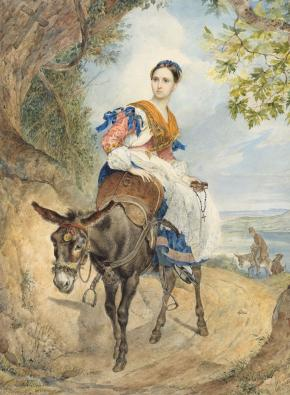
\includegraphics[width=\linewidth]{imagenes/dataset_examples/drawings.jpg}
        \caption*{Drawings}
    \end{subfigure}
    \begin{subfigure}[t]{0.3\textwidth}
        \centering
        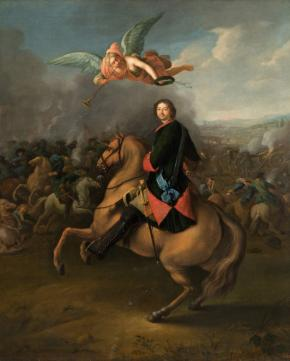
\includegraphics[width=\linewidth]{imagenes/dataset_examples/painting.jpg}
        \caption*{Painting}
    \end{subfigure}
    \begin{subfigure}[t]{0.3\textwidth}
        \centering
        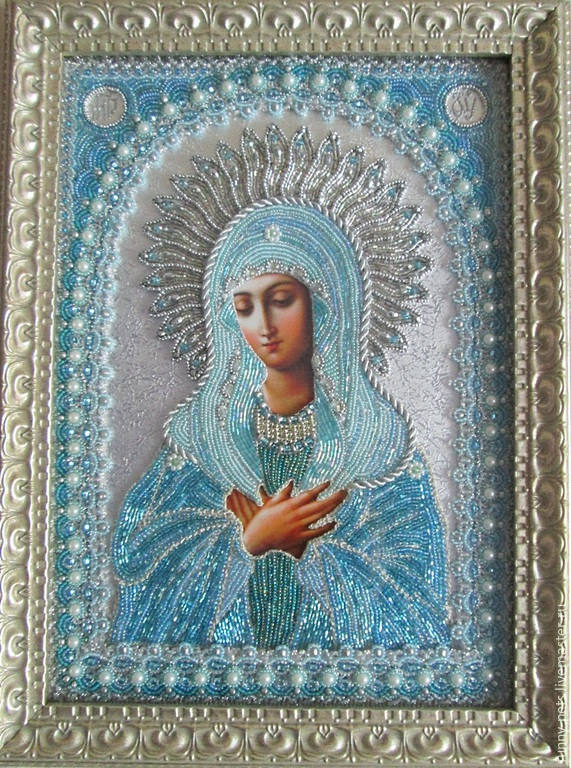
\includegraphics[width=\linewidth]{imagenes/dataset_examples/iconography.jpg}
        \caption*{Iconography}
    \end{subfigure}
    \begin{subfigure}[t]{0.3\textwidth}
        \centering
        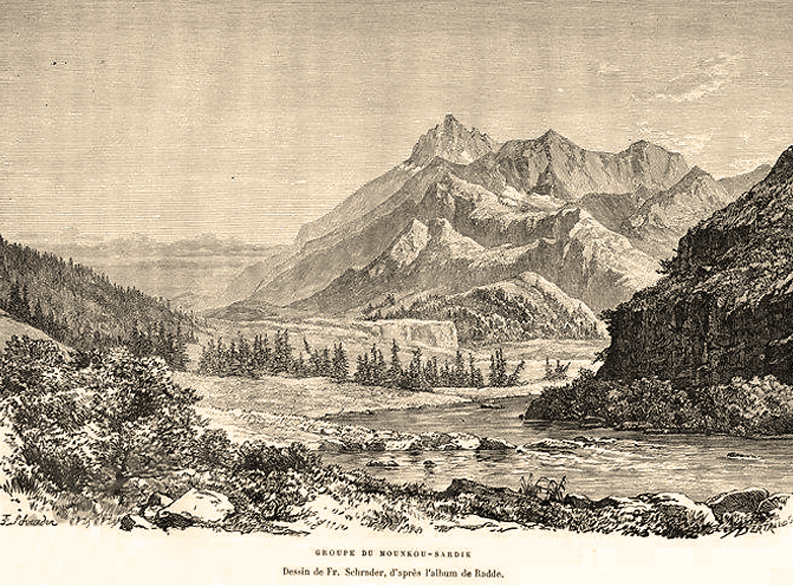
\includegraphics[width=\linewidth]{imagenes/dataset_examples/engraving.jpg}
        \caption*{Engraving}
    \end{subfigure}
    \begin{subfigure}[t]{0.3\textwidth}
        \centering
        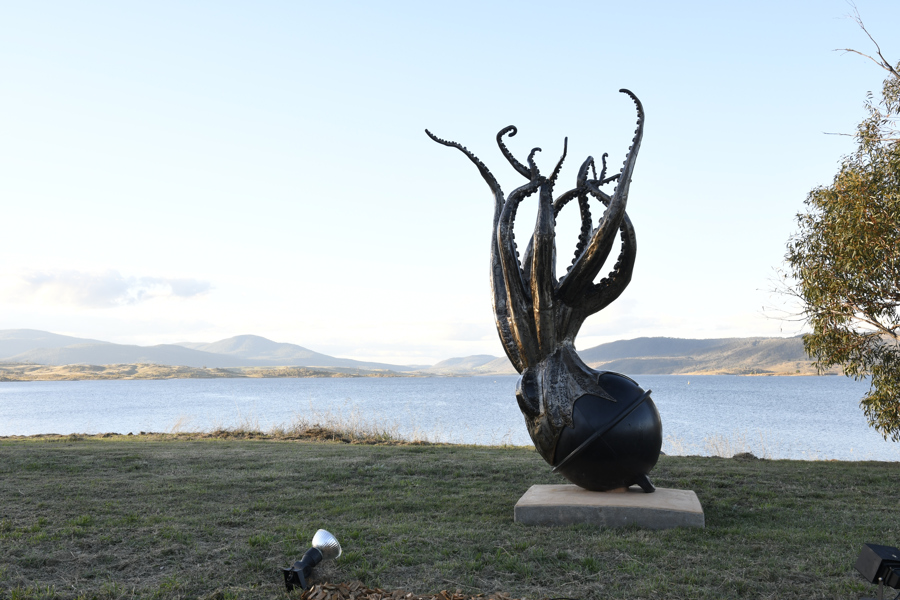
\includegraphics[width=\linewidth]{imagenes/dataset_examples/sculpture.jpg}
        \caption*{Sculpture}
    \end{subfigure}
    \caption{Ejemplos de clases en el dataset \texttt{PAINTING}}
    \label{fig:ejemplos-painting}
\end{figure}

En la figura~\ref{fig:ejemplos-painting} se han mostrado una imagen de cada una de las clases del dataset \texttt{PAINTING},
para que se pueda observar la variabilidad de las imágenes.

\subsubsection{Estructura del Dataset}
\begin{figure}[ht]
    \centering
    \begin{forest}mydirstyle
        [Dataset
            [Train (originalmente training\_set)
                [drawings
                            [image1.jpg]
                            [image2.jpg]
                            [\dots]
                    ]
                    [paintings
                            [image1.jpg]
                            [image2.jpg]
                            [\dots]
                    ]
                    [sculptures]
                    [engravings]
                    [iconography]
            ]
            [Test (originalmente validation\_set)
                [drawings]
                    [paintings]
                    [sculptures]
                    [engravings]
                    [iconography]
            ]
        ]
    \end{forest}
    \caption{Estructura de carpetas del dataset \texttt{PAINTING}}
    \label{fig:estructura-painting}
\end{figure}

Como se puede observar en la Figura~\ref{fig:estructura-painting}, las imágenes están organizadas en directorios según su categoría artística,
que en este caso corresponden a las distintas clases del dataset, previamente divididas en conjuntos de entrenamiento y prueba.

\subsubsection{Formato de los Datos}
Todas las imágenes están en formato JPEG (\texttt{.jpg}) y presentan variaciones en resolución y dimensiones.
Se han aplicado técnicas de preprocesamiento para homogenizar las características de las imágenes.

\subsubsection{Uso del Dataset}
Este dataset se ha utilizado para entrenar y evaluar modelos de clasificación de imágenes en un entorno diferente al
RPS\@.
Con este dataset, se ha comprobado el funcionamiento para evaluar los algoritmos con un dataset un poco mas complejo
que el RPS, con un par de clases más y con un número mayor de imágenes.

\subsubsection{Correcciones en la División de Datos}
Observando los tamaños de la división de los datos, y teniendo en cuenta que la divisón de los datos suele ser en train
y test, se ha decidido por renombrar las particiones de \texttt{valid} por \texttt{test} para que corresponda
correctamente con su propósito.
Y el set de validation lo he obtenido separando el set de train, normalmente haciendo una división 80\% test y 20\%
valid.

\subsubsection{Acceso al Dataset}
Inicialmente, el dataset se descargó desde Kaggle~\cite{OriginalArtImages}

Sin embargo, debido a la presencia de archivos innecesarios y algunas imágenes corruptas, se opta por una versión
limpia disponible en Kaggle~\cite{CleanedArtImages}.

\subsubsection{Licencia y Uso}
Antes de su uso, se revisaron los términos y condiciones establecidos en la página de Kaggle para asegurar el
cumplimiento con las licencias y restricciones aplicables.

\subsection{Comparación entre datasets}\label{subsec:comparacion-entre-datasets}
Gracias a la tabla~\ref{tab:resumen-datasets} que con las características más relevantes de los datasets utilizados,
permite entender mejor la complejidad relativa de cada conjunto y cómo pueden influir en el comportamiento de los algoritmos:

\begin{table}[htp]
    \centering
    \resizebox{\textwidth}{!}{
        \begin{tabular}{|l|c|c|c|c|}
            \hline
            \textbf{Dataset}      & \textbf{Nº Imágenes} & \textbf{Nº Clases} & \textbf{Formato} & \textbf{Tamaño Imagen} \\
            \hline
            Rock, Paper, Scissors & \textasciitilde2.500 & 3                  & JPG              & 300×300 px             \\
            PAINTING              & \textasciitilde9.000 & 5                  & JPG              & Variable               \\
            \hline
        \end{tabular}
    }
    \caption{Resumen comparativo de los datasets utilizados}
    \label{tab:resumen-datasets}
\end{table}

La selección de estos dos datasets responde a la necesidad de evaluar los algoritmos meméticos en distintos niveles de complejidad.
El dataset \textbf{Rock, Paper, Scissors} se utilizó en las primeras fases del proyecto como punto de partida,
ya que ofrecía un entorno sencillo y controlado, con un número reducido de clases y una estructura equilibrada.
Esto permite desarrollar las bases del sistema y probar las primeras versiones de los algoritmos de manera más ágil y con menor complejidad computacional.

Por su parte, el dataset \textbf{PAINTING} se empleó posteriormente para validar el comportamiento de los algoritmos en un entorno más exigente.
Al incluir cinco categorías de arte con distintos estilos visuales, este conjunto introdujo una mayor variabilidad tanto semántica como estructural,
lo que permite evaluar la robustez y capacidad de generalización de las soluciones desarrolladas.


\section{Diseño de los experimentos}\label{sec:diseño-de-los-experimentos}
La fase experimental se organiza en varias etapas.
Inicialmente se opta por un dataset simple (\textit{Rock, Paper, Scissors}) para validar el funcionamiento general del sistema.
Posteriormente, se realizan pruebas con datasets más exigentes.
Los experimentos se repiten utilizando diferentes porcentajes iniciales de datos (10\%, 25\%, 50\% y 75\%)
para estudiar cómo afecta la cantidad de datos seleccionados al rendimiento del modelo.

Con el fin de asegurar la consistencia entre ejecuciones experimentales, se aplican las medidas de control de reproducibilidad
descritas en el \hyperref[sec:consideraciones-de-optimizacion]{Apartado~\ref*{sec:consideraciones-de-optimizacion}}.
Esto permite comparar algoritmos en condiciones homogéneas, evitando variaciones indeseadas causadas por componentes aleatorios del entorno de ejecución.

En cada prueba, se realizan 5 ejecuciones en paralelo, cada una utilizando una semilla distinta.
Esta estrategia permite obtener resultados promedio más robustos frente a la aleatoriedad del proceso evolutivo, asegurando una mayor fiabilidad estadística.

Los apartados siguientes explican con mayor detalle el procedimiento adoptado para llevar a cabo dichas ejecuciones.


\section{Procedimiento de Ejecución y Evaluación}\label{sec:procedimiento-de-ejecucion-y-evaluacion}
Para garantizar la consistencia y objetividad en la comparación entre algoritmos, se diseñan un procedimiento experimental sistemático y replicable.
Cada ejecución se realizó bajo las mismas condiciones computacionales y utilizando los mismos parámetros base,
salvo en aquellos casos en que se deseaba estudiar una variación concreta, como los distintos porcentajes iniciales o el uso de metaheurísticas con porcentajes libres.

\subsection{Métricas de Evaluación}\label{sec:metricas-de-evaluacion}
Para evaluar el rendimiento de los modelos se utilizaron métricas estándar como \textbf{accuracy}, \textbf{precisión}, \textbf{recall} y \textbf{F1-score},
calculadas sobre el conjunto de validación tras cada evaluación.
Para una definición formal de estas métricas, véase el \hyperref[sec:metricas-evaluacion]{Apartado~\ref*{sec:metricas-evaluacion}}.

Estas métricas se calcularon utilizando las funciones de \texttt{scikit-learn}, a partir de las predicciones del modelo y las etiquetas
reales correspondientes a los subconjuntos de imágenes seleccionados por cada algoritmo.

\subsection{Evaluaciones por Ejecución}\label{sec:evaluaciones-por-ejecucion}
Se buscó un equilibrio entre la cantidad de evaluaciones y el tiempo de ejecución, permitiendo una exploración suficiente del espacio de soluciones sin comprometer la eficiencia computacional.
Por ello, cada algoritmo se configura para realizar un máximo de 100 evaluaciones por ejecución,
independientemente del tipo de algoritmo utilizado, con el fin de mantener la equidad comparativa.

Cada evaluación consiste en generar un subconjunto de datos, entrenar el modelo correspondiente (ResNet50 o MobileNetV2),
y calcular su \textit{fitness} de acuerdo con las métricas mencionadas.

El número de evaluaciones sin mejora también se monitoriza para aplicar criterios de parada anticipada,
explicados previamente en el \hyperref[sec:consideraciones-de-optimizacion]{Apartado~\ref*{sec:consideraciones-de-optimizacion}},
reduciendo así el tiempo computacional en caso de estancamiento.

\subsection{Repeticiones y Semillas}\label{sec:repeticiones-y-semillas}
Con el objetivo de obtener resultados estadísticamente significativos y reducir el efecto de la aleatoriedad,
cada configuración experimental se ejecuta 5 veces, utilizando 5 semillas distintas.
Los resultados presentados en las tablas y gráficos corresponden a la media de esas ejecuciones,
junto con medidas de dispersión cuando procede, como los boxplots.

Cabe destacar que, en el caso de los boxplots, en lugar de representar la media de las 5 ejecuciones por configuración,
se opta por incluir todos los valores individuales obtenidos con las distintas semillas.
Esta decisión permite visualizar una distribución más realista del comportamiento de cada algoritmo,
resaltando mejor la mediana, así como los valores máximos y mínimos alcanzados durante las ejecuciones.

\subsection{Tiempos de Ejecución}\label{sec:tiempos-de-ejecucion}
Cada evaluación implica entrenar un modelo desde cero, por lo que los tiempos de ejecución son considerables.
Por ejemplo, una ejecución completa con 100 evaluaciones puede tardar entre 30 minutos y 2 horas,
dependiendo del algoritmo y del modelo utilizado.

Los algoritmos más complejos, como el memético o las versiones con reinicio poblacional,
requieren un mayor tiempo de ejecución debido a las operaciones adicionales de mejora local o regeneración de población.


\section{Visualización de resultados}\label{subsec:visualizacion-de-resultados}
Para facilitar la comparación entre algoritmos, en el resto del trabajo se incluyen representaciones gráficas de los
resultados obtenidos mediante \textbf{boxplots} y \textbf{barplots}.
Ambos tipos de gráficos permiten visualizar el comportamiento global de cada algoritmo a partir de múltiples ejecuciones con distintas semillas.

\textbf{Los boxplots} (diagramas de caja) muestran la distribución estadística de los valores obtenidos.
En la Figura~\ref{fig:boxplot-explicado} se presenta un ejemplo anotado que ilustra las distintas partes de este tipo de gráfico.
La línea central de la caja representa la \textbf{mediana},
mientras que los bordes inferior y superior corresponden al \textbf{primer cuartil} (Q1) y \textbf{tercer cuartil} (Q3), respectivamente.
La diferencia entre ellos define el \textbf{rango intercuartílico} (\textit{IQR}), que contiene el 50\% central de los valores.
Las líneas que se extienden desde la caja (conocidas como \textit{bigotes}) alcanzan típicamente hasta 1.5 veces el IQR.
Los puntos que quedan fuera de ese rango se consideran \textbf{valores atípicos}, lo que permite detectar ejecuciones excepcionales.
Esta representación es especialmente útil para comparar la tendencia central, la dispersión y la estabilidad de los resultados obtenidos por los distintos algoritmos.

\begin{figure}[H]
    \centering
    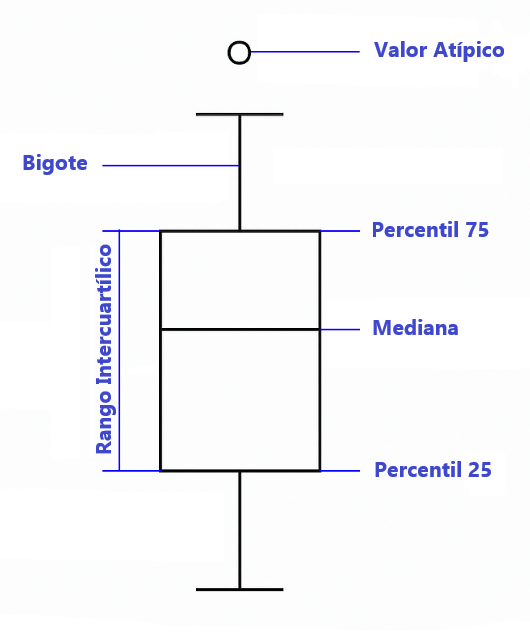
\includegraphics[width=0.45\textwidth]{imagenes/boxplot-explicado}
    \caption{Ejemplo de boxplot explicado.}
    \label{fig:boxplot-explicado}
\end{figure}

\textbf{Los barplots} (gráficos de barras), por su parte, se emplean para representar valores agregados como medias o proporciones,
y son útiles para observar cómo varía una métrica concreta entre distintos algoritmos, modelos o configuraciones.
Además, los barplots muestran unas barras de error que indica la desviación estándar de los valores,
lo que permite apreciar la variabilidad de los resultados obtenidos en las distintas ejecuciones.

\textbf{Los scatter plots} (diagramas de dispersión) permiten visualizar de forma conjunta la relación entre el 
porcentaje inicial de datos seleccionados y el porcentaje final alcanzado tras aplicar los algoritmos.
En estos gráficos, cada punto representa una ejecución concreta, donde:

\begin{itemize}
    \item El eje \textbf{X} indica el \textbf{Porcentaje Inicial} de datos usados.
    \item El eje \textbf{Y} muestra el \textbf{Porcentaje Final} de datos seleccionados por el algoritmo tras la ejecución.
    \item El \textbf{color} y el \textbf{tamaño} de los puntos reflejan el \textbf{accuracy} alcanzado: los puntos más grandes 
    y con tonos más intensos corresponden a ejecuciones con mayor precisión.
\end{itemize}

Además, cada punto se conecta mediante líneas de guía horizontales y verticales a los ejes, lo que facilita la interpretación de su posición exacta.
Estas líneas ayudan a identificar rápidamente los valores individuales en ambos ejes, mejorando la legibilidad del gráfico.

Este tipo de visualización es especialmente útil para analizar cómo los algoritmos ajustan el tamaño del subconjunto de datos en función de las condiciones iniciales, 
y cómo esta selección influye en la precisión del modelo.
Permite detectar patrones como agrupamientos de soluciones o dispersiones, y observar cómo ciertas configuraciones iniciales tienden a producir mejores o peores resultados.


\section{Nomenclatura simplificada de los algoritmos}\label{subsec:nomenclatura-algoritmos}
Para facilitar la lectura de las tablas y gráficos presentados a lo largo de este trabajo,
se opta por utilizar abreviaciones consistentes para referirse a los algoritmos implementados.
Estas abreviaciones permiten condensar la información visualmente sin perder la claridad en la interpretación de los resultados.

La correspondencia entre el nombre completo de cada algoritmo y su abreviatura se muestra en la Tabla~\ref{tab:nombres-algoritmos}.

\begin{table}[htp]
    \centering
    \begin{tabular}{ll}
        \toprule
        \textbf{Nombre Completo del Algoritmo}                 & \textbf{Abreviatura} \\
        \midrule
        Aleatorio (Random Search)                              & RS                   \\
        Búsqueda Local (Local Search)                          & LR                   \\
        Búsqueda Local Libre                                   & LR-F                 \\
        Algoritmo Genético                                     & GEN                  \\
        Genético con Cruce Ponderado (Weighted Crossover)      & WC                   \\
        Genético con Mutación Adaptativa (Adaptive Mutation)   & AM                   \\
        Genético con Mutación Adaptativa Libre                 & AM-F                 \\
        Genético con Reinicio Poblacional (Population Restart) & PR                   \\
        Algoritmo Memético                                     & MEM                  \\
        Algoritmo Memético Libre                               & MEM-F                \\
        \bottomrule
    \end{tabular}
    \caption{Nomenclatura simplificada de los algoritmos.}
    \label{tab:nombres-algoritmos}
\end{table}

A partir de este punto, todas las tablas y gráficos del documento utilizarán estas abreviaturas para referirse a los algoritmos,
mejorando la legibilidad de los resultados y facilitando la interpretación de las comparativas entre métodos.


\section{Estructura de las Tablas de Resultados}\label{subsec:estructura-tablas}
En los siguientes capítulos, algunos resultados obtenidos a partir de los experimentos se presentan de forma tabulada para facilitar la
comprensión y el análisis comparativo entre algoritmos, modelos y configuraciones.
Estas tablas recogen las métricas de rendimiento clave obtenidas a lo largo de las distintas ejecuciones.

Las columnas principales que pueden aparecer en las tablas son las siguientes:
\begin{itemize}
    \item \textbf{Porcentaje Inicial}: Indica el porcentaje inicial de datos seleccionados por el algoritmo para cada ejecución.
          Este valor permite analizar cómo varía el rendimiento del modelo en función de la cantidad de datos utilizados.
    \item \textbf{Evaluaciones Realizadas}: Número total de evaluaciones efectuadas por el algoritmo en cada configuración.
          Generalmente, este valor se fija en 100, salvo en casos concretos como la evaluación con el 100\% del conjunto de datos.
    \item \textbf{Duración Total}: Tiempo total requerido para completar todas las evaluaciones de una configuración, expresado en formato \textit{horas:minutos:segundos}.
          Este campo ayuda a comparar la eficiencia computacional de los algoritmos.
          Se obtiene a partir de las distintas ejecuciones del algoritmo con diferentes semillas.
    \item \textbf{Duración por Evaluación}: Tiempo necesario para realizar un único entrenamiento, permitiendo evaluar la rapidez de cada modelo de forma precisa.
          Este valor se calcula dividiendo la duración total entre el número de evaluaciones realizadas.
    \item \textbf{Accuracy (Avg)}: Precisión media alcanzada, expresada en porcentaje, calculada sobre el conjunto de validación.
          Se obtiene a partir de las distintas ejecuciones del algoritmo con diferentes semillas.
    \item \textbf{Precision (Avg)}: Media de la precisión por clase (macro promedio), que refleja la proporción de verdaderos positivos entre todas las predicciones positivas para cada clase.
    \item \textbf{Recall (Avg)}: Media del \emph{recall} por clase, que indica la proporción de verdaderos positivos entre todas las instancias reales de cada clase.
    \item \textbf{F1-score (Avg)}: Media armónica entre precisión y \emph{recall}, calculada por clase y luego promediada (macro promedio).
          Es una métrica clave para problemas multiclase.
\end{itemize}

En algunas tablas, los resultados se agrupan por \textbf{modelo de red neuronal} o por \textbf{porcentaje inicial},
permitiendo comparar directamente su rendimiento bajo las mismas condiciones experimentales y facilitando el análisis del impacto de la cantidad de datos seleccionados.

Por último, aclarar que las abreviaturas de los algoritmos empleadas en las tablas corresponden a las definidas en la Tabla~\ref{subsec:nomenclatura-algoritmos},
para mejorar la legibilidad de los resultados y simplificar las comparaciones.

Las tablas están diseñadas para ofrecer una visión clara, precisa y estructurada del impacto de cada configuración experimental en el rendimiento final de los modelos.
Esta información es fundamental para evaluar la eficacia de las estrategias de reducción de datos implementadas en este trabajo.


\section{Parámetros de los Algoritmos y del Entrenamiento}\label{subsec:parametros-algoritmos}
En este apartado se describen los principales parámetros utilizados en el desarrollo de los algoritmos de
selección de instancias y en el proceso de entrenamiento de los modelos de clasificación.
La correcta configuración de estos parámetros es fundamental para asegurar un equilibrio entre la calidad de los resultados y la eficiencia computacional.

\subsection{Parámetros Generales de los Algoritmos}\label{subsec:parametros-generales-algoritmos}
\begin{itemize}
    \item \textbf{Porcentaje inicial de selección} (\texttt{initial\_percentage}): Define el porcentaje inicial de datos seleccionados para cada ejecución.
          Se han evaluado valores como 10\%, 25\%, 50\% y 75\%.
    \item \textbf{Número máximo de evaluaciones} (\texttt{max\_evaluations}): Límite de iteraciones para cada algoritmo, generalmente fijado en 100.
    \item \textbf{Número máximo de evaluaciones sin mejora} \\(\texttt{max\_evaluations\_without\_improvement}):
          Controla la parada anticipada si no se mejora el mejor resultado durante un número consecutivo de iteraciones.
    \item \textbf{Métrica de optimización} (\texttt{metric}): Métrica utilizada para calcular el fitness,
          siendo \texttt{accuracy} la más habitual, aunque también se soportan \texttt{f1-score} y otras métricas.
    \item \textbf{Modelo de red neuronal} (\texttt{model\_name}): Arquitectura utilizada para la clasificación, como \texttt{ResNet50} o \texttt{MobileNetV2}.
\end{itemize}

\subsection{Parámetros del Entrenamiento de Modelos}\label{subsec:parametros-entrenamiento-modelos}

\begin{itemize}
    \item \textbf{Tamaño del batch} (\texttt{batch\_size}): Número de imágenes procesadas simultáneamente durante el entrenamiento.
          Se fija en 32 para equilibrar tiempo y estabilidad.
    \item \textbf{Número de épocas} (\texttt{num\_epochs}): Número de veces que el modelo se entrena sobre el subconjunto seleccionado.
          Se utiliza 10 para cada evaluación.
    \item \textbf{Tasa de aprendizaje} (\texttt{learning\_rate}): Controla la magnitud de los ajustes de pesos durante el entrenamiento.
          Se establece en 0.001 para la capa final, manteniendo el resto de la red congelada.
    \item \textbf{Dispositivo de ejecución} (\texttt{device}): Determina si el entrenamiento se realiza en CPU o GPU.
          Se prioriza el uso de GPU cuando está disponible.
\end{itemize}

\subsection{Parámetros Específicos por Algoritmo}\label{subsec:parametros-especificos-algoritmos}

\textbf{Random Search:}
\begin{itemize}
    \item No utiliza parámetros adicionales, ya que la selección de instancias es completamente aleatoria.
\end{itemize}

\textbf{Búsqueda Local:}
\begin{itemize}
    \item \textbf{Tamaño del vecindario} (\texttt{neighbor\_size}): Número de imágenes modificadas en cada generación de vecino, fijado en 10.
    \item \textbf{Ajuste dinámico del tamaño del subconjunto} (\texttt{adjust\_size}): Permite variar el tamaño total de las soluciones en las versiones libres.
\end{itemize}

\textbf{Algoritmos Genéticos:}
\begin{itemize}
    \item \textbf{Tamaño de la población} (\texttt{population\_size}): Número de individuos en cada generación, generalmente 10.
    \item \textbf{Tamaño del torneo} (\texttt{tournament\_size}): Número de soluciones evaluadas para seleccionar padres en el cruce, fijado en 3.
    \item \textbf{Tasa de mutación} (\texttt{mutation\_rate}): Probabilidad de modificar aleatoriamente las soluciones, fijado en 0.1.
    \item \textbf{Ajuste dinámico del tamaño del subconjunto} (\texttt{adjust\_size}): Permite modificar el tamaño del subconjunto durante la ejecución.
\end{itemize}

\textbf{Algoritmo Memético:}
\begin{itemize}
    \item \textbf{Probabilidad de búsqueda local} (\texttt{local\_search\_probability}): Probabilidad de aplicar una búsqueda local a un individuo, fijada en 0.2.
    \item \textbf{Número de evaluaciones de búsqueda local} \\(\texttt{local\_search\_evaluations}): Máximo de evaluaciones locales por individuo, fijado en 10.
    \item \textbf{Tamaño del vecindario en búsqueda local} \\(\texttt{local\_search\_neighbor\_size}): Número de cambios permitidos en cada iteración de búsqueda local.
          Fijado en 5.
    \item \textbf{Ajuste dinámico del tamaño del subconjunto} (\texttt{adjust\_size}): Permite modificar el tamaño del subconjunto durante la ejecución.
\end{itemize}

\subsection*{}
La combinación de estos parámetros permite un control detallado del proceso de selección de instancias y del entrenamiento de los modelos,
asegurando resultados reproducibles, eficientes y de calidad.

% !TeX root = ../proyecto.tex

\chapter{Resultados y Análisis}\label{ch:resultados-y-analisis}
En este capítulo se exponen los experimentos realizados y los resultados obtenidos en los distintos escenarios evaluados.
El objetivo principal fue analizar el rendimiento de los modelos entrenados con conjuntos de datos reducidos,
seleccionados mediante los distintos algoritmos desarrollados a lo largo del proyecto.



\section{Resultados con el conjunto completo}\label{sec:resultados-conjunto-completo}
Como punto de partida, se evalúa el rendimiento de los modelos convolucionales entrenados con el \textbf{100\%} del conjunto de datos.
Esta prueba sirve como referencia para contrastar los resultados obtenidos mediante las técnicas de reducción aplicadas posteriormente.
Se emplean los modelos \textbf{ResNet50} y \textbf{MobileNetV2}, y se miden las métricas de \textit{accuracy},
\textit{precision}, \textit{recall} y \textit{F1-score} sobre el conjunto de validación.

\begin{table}[htp]
    \centering
    \resizebox{\textwidth}{!}{
        \begin{tabular}{P{2cm} P{2.5cm} P{2.5cm} P{2.5cm} P{2cm}}
            \toprule
            \textbf{Duración por Eval.} & \textbf{Accuracy (Avg)} & \textbf{Precision (Avg)} & \textbf{Recall (Avg)} & \textbf{F1-score (Avg)} \\
            \midrule
            \multicolumn{5}{l}{\textbf{Modelo ResNet50}}                                                                                       \\
            \midrule
            00:02:42                    & 87,90\%                 & 88,96\%                  & 87,90\%               & 87,81\%                 \\
            \midrule
            \multicolumn{5}{l}{\textbf{Modelo MobileNet}}                                                                                      \\
            \midrule
            00:03:16                    & 78,60\%                 & 81,55\%                  & 78,60\%               & 77,68\%                 \\
            \bottomrule
        \end{tabular}
    }
    \caption{Comparativa de resultados del \textbf{100\%} con los modelos \textbf{ResNet50} y \textbf{MobileNet}.}
    \label{tab:resultados-100-resnet50-mobilenet}
\end{table}

\begin{figure}[htp]
    \centering
    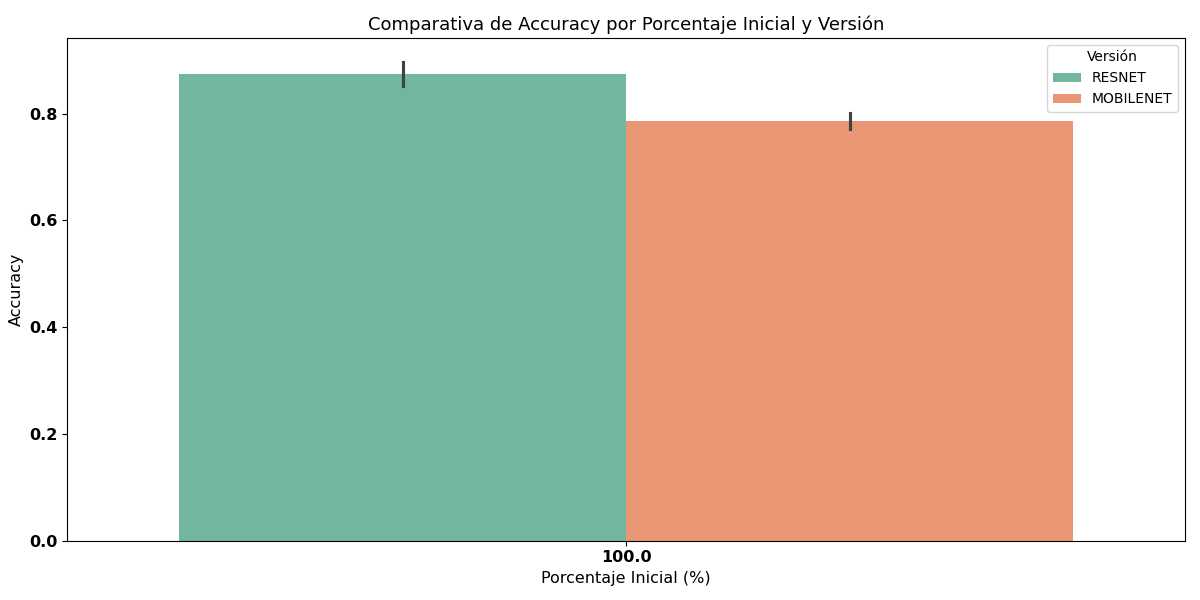
\includegraphics[width=0.95\textwidth]{imagenes/evaluaciones/comparacion_modelos_100.png}
    \caption{Comparación de \textit{accuracy} de los modelos ResNet50 y MobileNetV2 usando el 100\% del conjunto de datos.}
    \label{fig:comparacion_modelos_100}
\end{figure}

Los resultados presentados en la tabla~\ref{tab:resultados-100-resnet50-mobilenet}, y visualizados en la figura~\ref{fig:comparacion_modelos_100},
representan el rendimiento máximo alcanzable en condiciones ideales,
es decir, utilizando la totalidad del conjunto de datos sin aplicar técnicas de reducción.
Este escenario establece un techo de rendimiento que se utiliza como referencia para evaluar la eficacia de
los algoritmos de reducción de datos implementados en el resto del estudio.

En particular, se observa que \textbf{ResNet50} obtiene mejores resultados en todas las métricas evaluadas,
destacando especialmente en \textit{accuracy} y \textit{precision}, donde supera por más de 9 puntos porcentuales a \textbf{MobileNetV2}.
Esta superioridad en el rendimiento viene acompañada de un tiempo por evaluación ligeramente menor (\textbf{00:02:42} frente a \textbf{00:03:16}),
lo que indica una mayor eficiencia en la etapa de predicción.

Esta comparativa inicial permite establecer las bases para el análisis de los resultados obtenidos mediante las técnicas de reducción de datos,
sirviendo como referencia para valorar el impacto de las estrategias aplicadas en las secciones posteriores.


\section{Comparativa inicial de modelos}\label{sec:comparativa-inicial-modelos}
Antes de aplicar los algoritmos propuestos de reducción de datos, se considera fundamental realizar una comparativa inicial entre distintos
modelos de redes neuronales convolucionales para determinar cuál de ellos es el más adecuado para los experimentos.
Esta comparación permite identificar la arquitectura que ofrece un mejor equilibrio entre rendimiento y eficiencia computacional,
estableciendo una base sólida sobre la que construir los siguientes análisis.

Para llevar a cabo esta comparativa, se utiliza el enfoque aleatorio (\texttt{RS}) como estrategia de referencia.
Al seleccionar subconjuntos de datos de manera aleatoria, sin ninguna optimización, se obtiene una línea base que permiteevaluar el
comportamiento de cada modelo en condiciones controladas.
Esta línea base es especialmente valiosa, ya que ofrece una perspectiva realista del rendimiento mínimo esperable sin aplicar técnicas
avanzadas de reducción de datos, sirviendo como punto de partida para comparar las mejoras introducidas por los algoritmos posteriores.


\begin{table}[htp]
    \centering
    \resizebox{\textwidth}{!}{
        \begin{tabular}{P{2cm} P{2.5cm} P{2.5cm} P{2.5cm} P{2cm} P{2cm} P{2cm} P{2cm}}
            \toprule
            \textbf{Porcentaje Inicial} & \textbf{Evaluaciones Realizadas} & \textbf{Duración Total} & \textbf{Duración por Eval.} &
            \textbf{Accuracy (Avg)}     & \textbf{Precision (Avg)}         & \textbf{Recall (Avg)}   & \textbf{F1-score (Avg)}                                             \\
            \midrule
            \multicolumn{8}{l}{\textbf{Modelo ResNet50}}                                                                                                                   \\
            \midrule
            10\%                        & 100                              & 01:21:37                & 00:00:48                    & 85,16\% & 86,30\% & 85,16\% & 85,02\% \\
            25\%                        & 100                              & 01:28:14                & 00:00:52                    & 87,26\% & 88,13\% & 87,26\% & 87,02\% \\
            50\%                        & 100                              & 02:27:17                & 00:01:28                    & 88,49\% & 89,51\% & 88,49\% & 88,30\% \\
            75\%                        & 100                              & 03:52:41                & 00:02:19                    & 89,89\% & 90,53\% & 89,89\% & 89,70\% \\
            100\%                       & 1                                & -                       & 00:02:55                    & 87,42\% & 88,73\% & 87,42\% & 87,18\% \\
            \midrule
            \multicolumn{8}{l}{\textbf{Modelo MobileNet}}                                                                                                                  \\
            \midrule
            10\%                        & 100                              & 00:38:16                & 00:00:22                    & 81,34\% & 82,46\% & 81,34\% & 80,52\% \\
            25\%                        & 100                              & 01:18:22                & 00:00:47                    & 80,70\% & 81,90\% & 80,70\% & 79,90\% \\
            50\%                        & 100                              & 02:26:40                & 00:01:28                    & 80,86\% & 82,65\% & 80,86\% & 80,22\% \\
            75\%                        & 100                              & 03:05:48                & 00:01:51                    & 82,26\% & 84,16\% & 82,26\% & 81,67\% \\
            100\%                       & 1                                & -                       & 00:03:16                    & 78,60\% & 81,55\% & 78,60\% & 77,68\% \\
            \bottomrule
        \end{tabular}
    }
    \caption{Comparativa de resultados de la generación inicial utilizando el \texttt{RS} y el \texttt{100\%} con los modelos \texttt{ResNet50} y \texttt{MobileNet}.}
    \label{tab:resnet50-vs-mobilenet}
\end{table}

\begin{figure}[htp]
    \centeringñ
    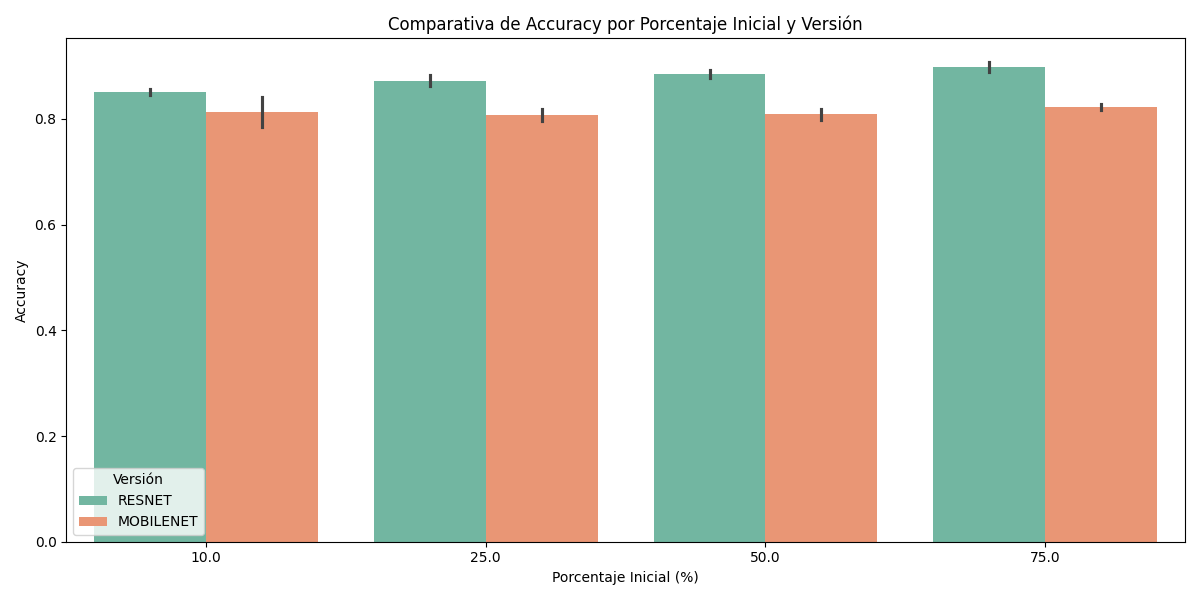
\includegraphics[width=0.95\textwidth]{imagenes/evaluaciones/comparacion_modelos.png}
    \caption{Diagrama de barras para comparar los modelos usando el \textit{accuracy} alcanzado por cada porcentaje inicial.}
    \label{fig:comparacion_modelos}
\end{figure}

\colorbox{yellow}{Volver a ejecutar los resultados para comprobar tiempos.}
Se realizan pruebas con distintos porcentajes iniciales de datos seleccionados aleatoriamente (10\%, 25\%, 50\%, 75\% y 100\%), utilizando tanto ResNet50 como MobileNetV2.
Los resultados obtenidos se presentan en la Tabla~\ref{tab:resnet50-vs-mobilenet}, que resume las métricas alcanzadas por cada modelo,
y en la Figura~\ref{fig:comparacion_modelos}, que muestra la comparación de los valores de \textit{accuracy} mediantes barras separados por los porcentajes iniciales.

Los resultados muestran que ResNet50 logra un mejor rendimiento en términos de \textit{accuracy}, \textit{precision}, \textit{recall} y \textit{F1-score}.
Sin embargo, este mejor rendimiento viene acompañado de un tiempo de entrenamiento considerablemente mayor.
Por su parte, MobileNetV2 ofrece una solución más eficiente en cuanto a tiempos de ejecución, a costa de una ligera pérdida de precisión,
lo que la convierte en una opción atractiva para entornos con recursos computacionales limitados.

En conjunto, esta comparativa inicial permite elegir MobileNetV2 como modelo principal para el resto de experimentos.
Aunque ResNet50 ofrece una precisión ligeramente superior, su elevado coste computacional no justifica su uso en las pruebas de reducción de datos,
donde la eficiencia es un factor clave.
Además, el uso del \texttt{RS} como referencia permite establecer un punto de comparación para evaluar las mejoras que los algoritmos propuestos aportarían sobre esta línea base.


\section{Resultados de la búsqueda local}\label{sec:resultados-busqueda-local}
Como se describe en el apartado correspondiente (ver \hyperref[sec:algoritmo-busqueda-local]{Sección~\ref*{sec:algoritmo-busqueda-local}}),
la búsqueda local permite mejorar progresivamente una solución inicial mediante pequeñas modificaciones guiadas por el rendimiento.
En este apartado se evalúa su efectividad como alternativa más estructurada frente al enfoque aleatorio, pero sin llegar a la complejidad de los algoritmos evolutivos.
Su inclusión busca analizar hasta qué punto una estrategia simple pero guiada puede generar subconjuntos de datos más representativos y consistentes.

\begin{figure}[htp]
    \centering
    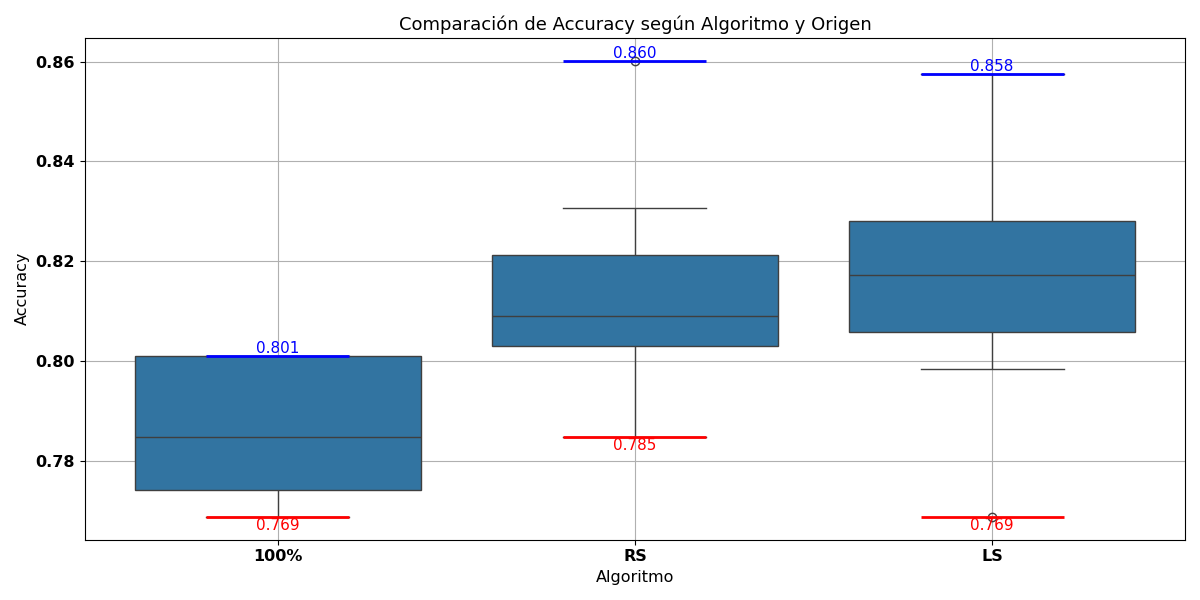
\includegraphics[width=1\textwidth]{imagenes/evaluaciones/comparacion_rs-ls.png}
    \caption{Boxplot comparando el \texttt{RS} con la \texttt{LS} usando \textit{accuracy}.}
    \label{fig:aleatorio-vs-busqueda-local}
\end{figure}
En la Figura~\ref{fig:aleatorio-vs-busqueda-local} se muestran los resultados mediante un boxplot que permite observar
la distribución completa de valores obtenidos en las distintas ejecuciones.

Se puede apreciar que el algoritmo de búsqueda local (\texttt{LS}) mejora claramente la mediana del \textit{accuracy} respecto al enfoque aleatorio (\texttt{RS}).
Mientras que el \texttt{RS} se sitúa en torno a una mediana de \textbf{0.787}, la \texttt{LS} alcanza una mediana superior, próxima a \textbf{0.818}.
Esta diferencia refleja una mayor capacidad del algoritmo local para generar subconjuntos más representativos y eficaces.

Además, los valores máximos que alcanzan ambos algoritmos son similares (en torno a \textbf{0.858}-\textbf{0.860}),
pero la \texttt{LS} muestra una dispersión más acotada hacia valores altos, lo que sugiere mayor estabilidad en sus resultados.
En cambio, el \texttt{RS} presenta una mayor dispersión hacia valores bajos y aunque presente una mayor sensibilidad a la aleatoriedad de las selecciones,
puede llegar a tener mejores valores mínimos, como se evidencia en su menor valor mínimo (\textbf{0.785} frente a \textbf{0.769} en \texttt{LS}),
pero siendo el de la \texttt{LS} un valor atípico.

Esto pone de manifiesto que, aunque el \texttt{RS} puede ocasionalmente alcanzar buenos resultados,
la \texttt{LS} ofrece una mejor consistencia y fiabilidad, con menos varianza entre ejecuciones y una tendencia general a obtener subconjuntos de entrenamiento más efectivos.


\section{Resultados del Algoritmo Genético}\label{sec:resultados-algoritmo-genetico}
Con el objetivo de superar las limitaciones observadas (como el riesgo de estancamiento o la exploración poco estructurada del espacio de soluciones)
se incorpora un enfoque evolutivo más completo: el algoritmo genético (\texttt{GA}), descrito en la Sección~\ref{sec:genetico-v1}, el cual sirve como punto de partida para explorar la
aplicación de estrategias metaheurísticas en la selección de subconjuntos representativos de imágenes.
Su estructura evolutiva, basada en selección por torneo, cruce e incorporación de mutación,
ofrece ya desde sus primeras versiones una capacidad superior para generalizar, en comparación con métodos más simples como la \texttt{LS}.

\begin{figure}[htp]
    \centering
    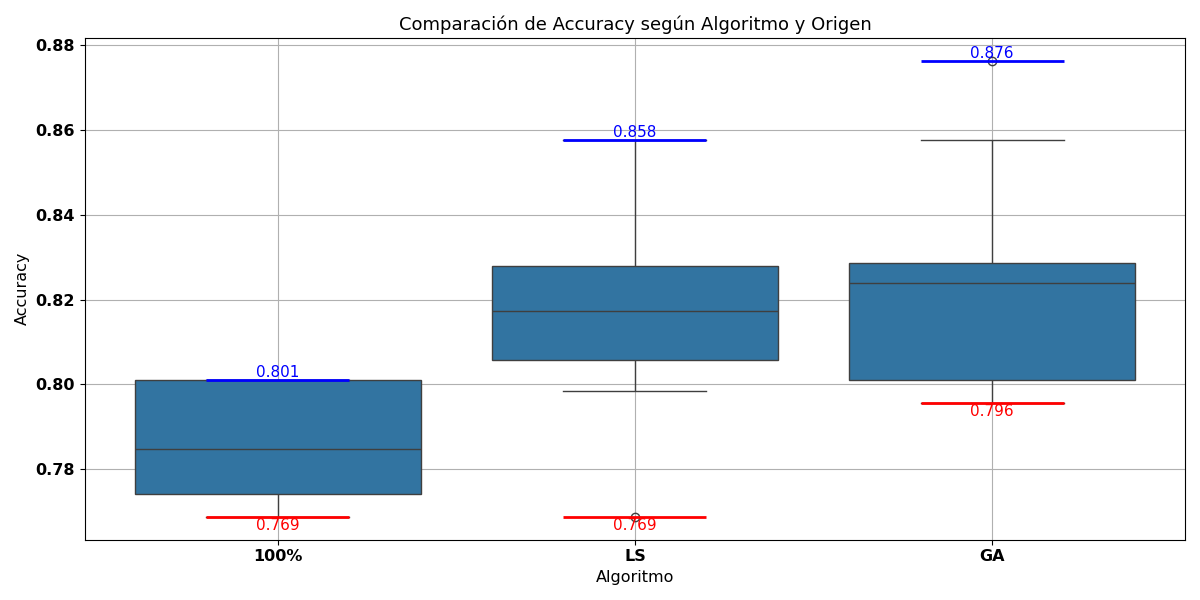
\includegraphics[width=1\textwidth]{imagenes/evaluaciones/comparacion_ls-ga.png}
    \caption{Boxplot comparando \texttt{LS} con \texttt{GA} usando \textit{accuracy}.}
    \label{fig:lr-vs-gen-v1}
\end{figure}

Tal como se observa en la Figura~\ref{fig:lr-vs-gen-v1}, el algoritmo genético (\texttt{GA}) consigue una \textbf{mediana de \textit{accuracy}} más alta que la búsqueda local (\texttt{LS}),
reflejando un rendimiento medio más consistente.
Además, presenta un valor máximo superior (alcanza hasta \textbf{0.876}), lo que evidencia su mayor potencial para encontrar soluciones de alta calidad.

No obstante, también se aprecia una ligera mayor dispersión en los resultados del \texttt{GA}, particularmente hacia los valores bajos.
Esto indica que, pese a su capacidad exploratoria, el \texttt{GA} puede generar soluciones poco efectivas si no se controlan adecuadamente ciertos operadores como el cruce o la mutación.
De hecho, su valor mínimo (\textbf{0.796}) es superior al de la \texttt{LS} en esta comparativa,
pero deja margen para mejoras en la presión selectiva o en mecanismos que eviten estancamientos.

La \texttt{LS}, por su parte, mantiene un comportamiento más estable, aunque con una mediana ligeramente inferior.
Su distribución es más concentrada y limitada en el extremo superior, lo que evidencia su carácter más explotador pero con menor capacidad para alcanzar soluciones óptimas globales.

Estos resultados sirven como evidencia empírica para continuar desarrollando nuevas versiones del \texttt{GA},
incorporando mejoras específicas en sus operadores con el fin de aprovechar su capacidad exploratoria y, al mismo tiempo, mitigar sus limitaciones.

\section{Mejorando el operador de cruce}\label{sec:incorporacion-cruce}
La primera mejora introducida al \texttt{GA} consiste en reemplazar el cruce aleatorio por un cruce ponderado,
donde se prioriza la contribución del progenitor con mayor \textit{fitness}.
Además, se incorpora una estrategia selectiva que conserva únicamente el mejor de los dos hijos generados en cada cruce.
Ambos cambios, explicados en detalle en la \hyperref[sec:genetico-v2]{Sección~\ref*{sec:genetico-v2}},
buscan aumentar la presión evolutiva y acelerar la convergencia hacia soluciones de mayor calidad,
evitando así que soluciones mediocres se propaguen innecesariamente en la población.

\begin{figure}[htp]
    \centering
    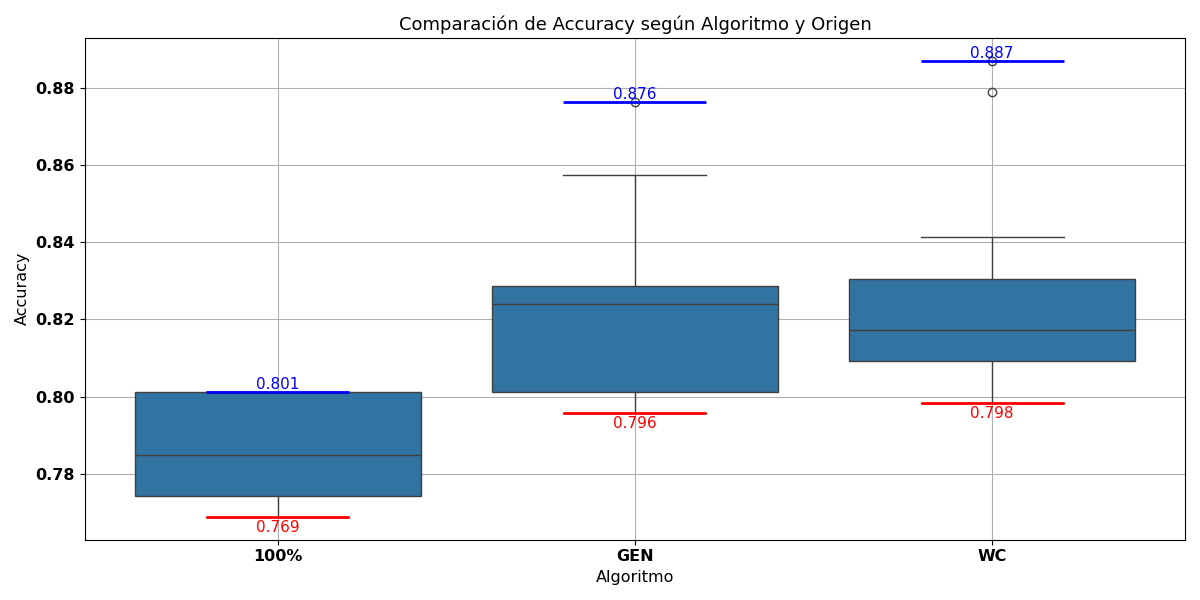
\includegraphics[width=1\textwidth]{imagenes/evaluaciones/operador-de-cruce.png}
    \caption{Boxplot de \textit{accuracy} comparando el \texttt{GA} y el \texttt{GA-WC}.}
    \label{fig:cruce_ponderado}
\end{figure}

Tal como se observa en la Figura~\ref{fig:cruce_ponderado}, esta modificación produce una mejora clara en la calidad y estabilidad de los resultados.
La versión con cruce ponderado (\texttt{GA-WC}) alcanza un valor máximo atípico superior (\textbf{0.887}),
aunque presenta una mediana más baja que la versión básica (\texttt{GA}).

Pero por otra parte, se aprecia una ligera reducción en la dispersión de los valores inferiores,
con un mínimo de \textbf{0.798} frente al \textbf{0.796} en la versión anterior, lo que sugiere una mayor consistencia.
Aunque el IQR (\hyperref[subsec:visualizacion-de-resultados]{Rango Intercuartílico}) sigue siendo amplio,
la acumulación de valores más cercanos al rango superior refleja una convergencia evolutiva más enfocada y menos dependiente del azar.

En conjunto, esta mejora en el cruce no solo permite una transferencia más eficiente de características ventajosas,
sino que también incrementa la presión selectiva sobre la calidad de las soluciones.
Esto se traduce en un comportamiento más robusto, menos propenso a resultados erráticos y con una mayor capacidad de exploración dirigida del espacio de soluciones.


\section{Mejorando el operador de mutación}\label{sec:mejorando-mutacion}
A partir de los resultados obtenidos con el \texttt{GA-WC}, se evalua una nueva versión en la que se introdujo una \textbf{mutación adaptativa}
(ver \hyperref[sec:genetico-mutacion]{Sección~\ref*{sec:genetico-mutacion}}).
A diferencia de la versión original con tasa fija, esta estrategia ajusta el número de intercambios en función del tamaño del subconjunto mutado,
lo que permite una mayor flexibilidad en escenarios de diferente escala.

\begin{figure}[htp]
    \centering
    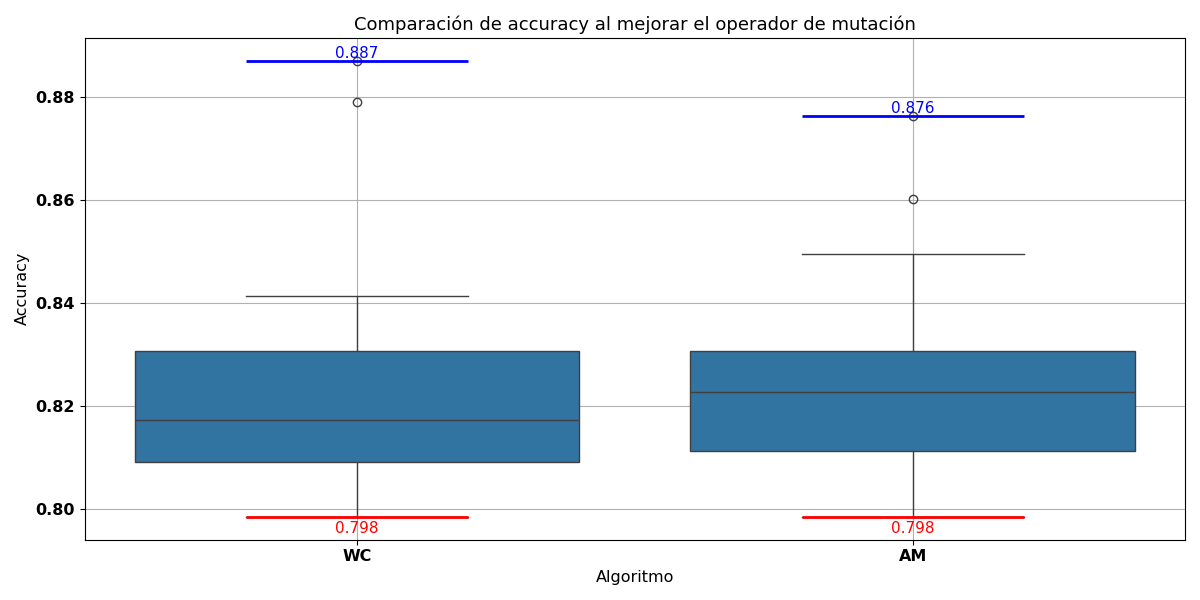
\includegraphics[width=1\textwidth]{imagenes/evaluaciones/mutacion-adaptativa.png}
    \caption{Comparación de \textit{accuracy} entre el \texttt{GA-WC} y el \texttt{GA-AM}.}
    \label{fig:mutacion-adaptativa}
\end{figure}

\begin{figure}[htp]
    \centering
    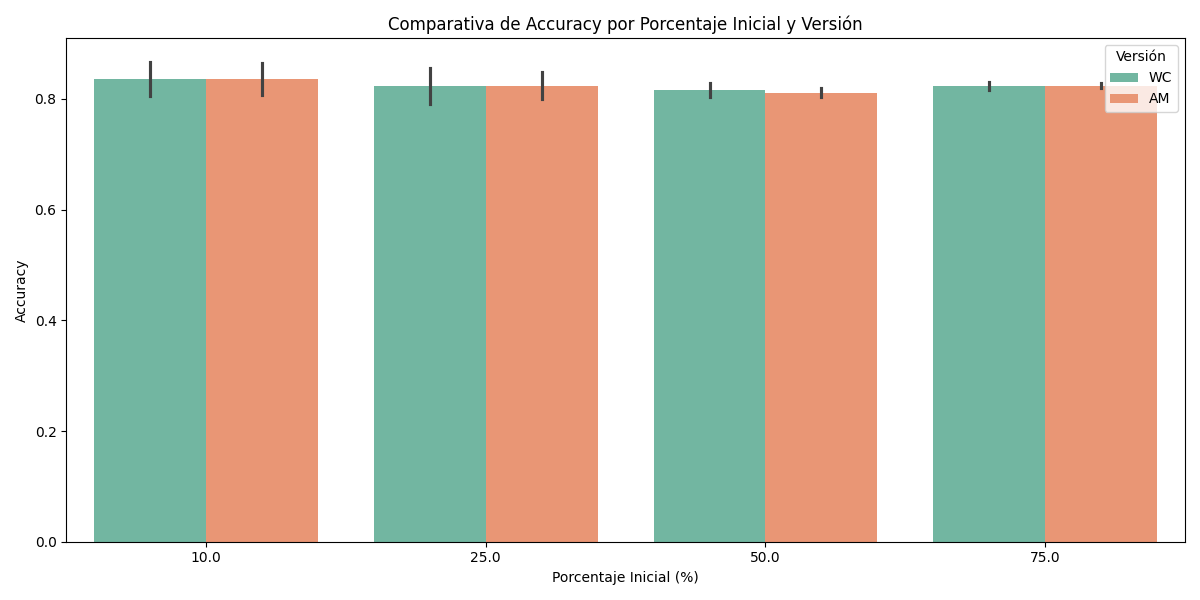
\includegraphics[width=1\textwidth]{imagenes/evaluaciones/mutacion-adaptativa_por_porcentaje.png}
    \caption{Diagrama de comparación usando el \textit{accuracy} entre el \texttt{GA-WC} Y el \texttt{GA-AM}, separados por porcentaje inicial.}
    \label{fig:mutacion-adaptativa-porcentaje}
\end{figure}

Como se aprecia en la Figura~\ref{fig:mutacion-adaptativa},
ambos algoritmos presentan distribuciones de \textit{accuracy} muy similares en términos de mediana e IQR.
El \texttt{GA-WC} mantiene un ligero máximo superior, alcanzando un \textbf{0.887} frente al \textbf{0.876} del \texttt{GA-AM}.
Sin embargo, el algoritmo con mutación adaptativa muestra una distribución más compacta en la parte central,
con menor dispersión hacia valores bajos, lo que sugiere una mayor consistencia entre ejecuciones.

La principal diferencia se observa en la robustez de los resultados: el \texttt{GA-AM} presenta una distribución más estable,
con menos valores atípicos y una mayor concentración de ejecuciones cerca del cuartil superior.
Este comportamiento indica una menor propensión a caídas abruptas de rendimiento y refuerza la idea de que la mutación
adaptativa mejora la estabilidad del proceso evolutivo.

Al analizar los resultados por porcentaje inicial (Figura~\ref{fig:mutacion-adaptativa-porcentaje}),
se confirma que el \texttt{GA-AM} mantiene una estabilidad más uniforme en todos los escenarios, mientras que el \texttt{GA-WC} muestra una mayor variabilidad,
especialmente en configuraciones con menor cantidad de datos.
Aunque las diferencias en \textit{accuracy} medio no son significativas, la menor dispersión y la reducción de valores extremos justifican la
preferencia por la versión adaptativa en contextos donde la fiabilidad es prioritaria.

En conjunto, la mutación adaptativa no genera una mejora radical en precisión media,
pero sí contribuye a una evolución más controlada y menos susceptible a degradaciones, favoreciendo una mayor consistencia en los resultados.
Además, al adaptarse al tamaño del subconjunto, evita configuraciones subóptimas que podrían surgir con una tasa fija de mutación,
lo que la hace especialmente adecuada para escenarios con escalas variables.

Esta mejora consolida la capacidad del algoritmo para equilibrar exploración y explotación,
y lo posiciona como una alternativa más robusta y estable en tareas de reducción de datos para aprendizaje profundo.


\section{Resultados del reinicio poblacional}\label{sec:resultados-reinicio-poblacional}
La última mejora realizada de los algoritmos genéticos (ver \hyperref[sec:genetico-v3]{Sección~\ref*{sec:genetico-v3}})
introduce una lógica de reinicio poblacional diseñada para evitar estancamientos evolutivos.
El algoritmo monitoriza el rendimiento del segundo mejor individuo, y si este no mejora durante dos generaciones consecutivas,
se aplica un reinicio parcial que conserva únicamente al mejor individuo de la población.

\begin{figure}[htp]
    \centering
    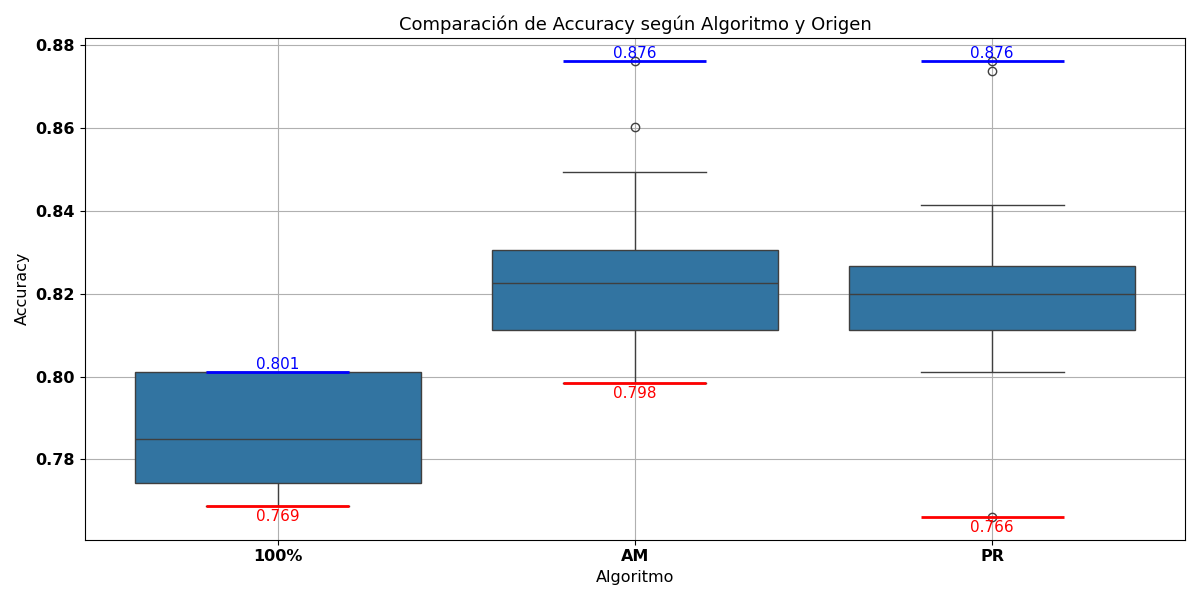
\includegraphics[width=1\textwidth]{imagenes/evaluaciones/reinicio-poblacional.png}
    \caption{Comparación de \textit{accuracy} entre el \texttt{GA-AM} y con \texttt{GA-PR}.}
    \label{fig:reinicio_poblacional}
\end{figure}
\begin{table}[htp]
    \centering
    \resizebox{\textwidth}{!}{
        \begin{tabular}{P{2cm} P{2cm} P{2.5cm} P{2.5cm} P{2.5cm} P{2.5cm} P{2cm} P{2cm} P{2cm} P{2cm} P{2cm} P{2.5cm} P{2.5cm}}
            \toprule
            \textbf{Algoritmo}    & \textbf{Duración Total} & \textbf{Duración por Eval.} & \textbf{Accuracy (Avg)} & \textbf{Precision (Avg)} &
            \textbf{Recall (Avg)} & \textbf{F1-score (Avg)} & \textbf{Evaluaciones}       & \textbf{Porc.Paper}     & \textbf{Porc.Rock}       & \textbf{Porc.Scissors}                                               \\
            \midrule
            \multicolumn{11}{l}{\textbf{10\%}}                                                                                                                                                                        \\
            \midrule
            GA-AM                 & 00:27:39                & 00:00:17                    & 83,66\%                 & 84,24\%                  & 83,66\%                & 83,09\% & 100 & 35,64\% & 30,87\% & 33,49\% \\
            GA-PR                 & 00:29:02                & 00:00:17                    & 81,93\%                 & 83,07\%                  & 81,93\%                & 81,19\% & 100 & 34,52\% & 32,14\% & 33,33\% \\
            \midrule
            \multicolumn{11}{l}{\textbf{25\%}}                                                                                                                                                                        \\
            \midrule
            GA-AM                 & 00:57:29                & 00:00:34                    & 82,42\%                 & 83,68\%                  & 82,42\%                & 81,78\% & 100 & 33,33\% & 32,54\% & 34,13\% \\
            GA-PR                 & 01:00:22                & 00:00:36                    & 82,64\%                 & 83,78\%                  & 82,64\%                & 81,96\% & 100 & 33,62\% & 33,27\% & 33,11\% \\
            \midrule
            \multicolumn{11}{l}{\textbf{50\%}}                                                                                                                                                                        \\
            \midrule
            GA-AM                 & 01:47:31                & 00:01:05                    & 81,13\%                 & 82,62\%                  & 81,13\%                & 80,41\% & 100 & 33,94\% & 32,76\% & 33,30\% \\
            GA-PR                 & 01:53:13                & 00:01:08                    & 81,24\%                 & 83,09\%                  & 81,24\%                & 80,59\% & 100 & 33,21\% & 33,20\% & 33,59\% \\
            \midrule
            \multicolumn{11}{l}{\textbf{75\%}}                                                                                                                                                                        \\
            \midrule
            GA-AM                 & 02:36:41                & 00:01:34                    & 82,42\%                 & 83,94\%                  & 82,42\%                & 81,85\% & 100 & 33,67\% & 33,11\% & 33,22\% \\
            GA-PR                 & 02:41:24                & 00:01:37                    & 82,69\%                 & 84,33\%                  & 82,69\%                & 82,06\% & 100 & 33,52\% & 33,44\% & 33,04\% \\
            \midrule
            \multicolumn{11}{l}{\textbf{100\%}}                                                                                                                                                                       \\
            \midrule
            100\%                 & --                      & 00:03:16                    & 78,60\%                 & 81,55\%                  & 78,60\%                & 77,68\% & 1   & 33,33\% & 33,33\% & 33,33\% \\
            \bottomrule
        \end{tabular}
    }
    \caption{Resultados de los algoritmos \texttt{GA-AM} y \texttt{GA-PR} por porcentaje inicial.}
    \label{tab:resultados-am-pr-porcentaje}
\end{table}

Los resultados, mostrados en la Figura~\ref{fig:reinicio_poblacional} y la Tabla~\ref{tab:resultados-am-pr-porcentaje},
permiten extraer varias conclusiones relevantes.
En primer lugar, el \textbf{valor máximo de accuracy} es idéntico para \texttt{GA-AM} y \texttt{GA-PR}, alcanzando ambos un \textbf{0.876},
lo que sugiere que el reinicio no favorece la aparición de soluciones de mayor calidad.
Por el contrario, el \textbf{valor mínimo de accuracy} observado en \texttt{GA-PR} (\textbf{0.766}) es notablemente más bajo que el de \texttt{GA-AM} (\textbf{0.798}),
lo que indica una mayor propensión a obtener ejecuciones de bajo rendimiento cuando se utiliza la estrategia de reinicio.

La distribución general de resultados revela que el \texttt{GA-PR} no logra una reducción significativa en la dispersión de los valores:
aunque los cuartiles y medianas de \texttt{GA-AM} y \texttt{GA-PR} son similares, se observa un leve desplazamiento hacia valores ligeramente más bajos en \texttt{GA-PR},
lo cual es especialmente evidente en el escenario de menor porcentaje inicial (10\%).
Esta tendencia sugiere que el reinicio poblacional, al reintroducir diversidad de forma abrupta,
puede generar soluciones subóptimas que no contribuyen de manera sustancial a mejorar la población.

La tabla de resultados~\ref{tab:resultados-am-pr-porcentaje} respalda estas observaciones: en promedio,
el algoritmo \texttt{GA-AM} presenta una ligera superioridad en precisión media (\textbf{83,66\%} frente a \textbf{81,93\%} en el 10\%), así como en F1-score y recall.
Estas diferencias, aunque no drásticas, son consistentes en la mayoría de los escenarios.
Además, las métricas de distribución de clases y las duraciones de ejecución son prácticamente equivalentes entre \texttt{GA-AM} y \texttt{GA-PR},
lo que refuerza la idea de que el impacto del reinicio poblacional no justifica su complejidad añadida.

En resumen, aunque el reinicio poblacional busca aumentar la exploración y evitar el estancamiento,
en esta implementación concreta no aporta mejoras tangibles en términos de precisión ni estabilidad,
e incluso puede introducir soluciones más erráticas en ciertas ejecuciones.

\section{Resultados con versiones libres}\label{sec:resultados-versiones-libres}
Como parte de la evolución de los algoritmos desarrollados, se propone la creación de \textbf{versiones libres},
en las que el tamaño del subconjunto seleccionado no permanece fijo durante la ejecución, sino que puede ajustarse de forma dinámica en función de las decisiones evolutivas.
Esta flexibilidad permite que los algoritmos modifiquen el número de datos utilizados a medida que avanzan las generaciones,
adaptándose de manera más natural a las características del problema.

Para evaluar el impacto de esta modificación, se generan versiones libres tanto para el algoritmo de búsqueda local (\texttt{LS})
como para el algoritmo con mutación adaptativa (\texttt{GA-AM}).
En el caso de la \texttt{LS}, además, se incorpora una variación adicional: el porcentaje inicial de imágenes no es fijo,
sino que se selecciona aleatoriamente en cada ejecución, introduciendo así un mayor grado de aleatoriedad y diversidad en el proceso.


\begin{figure}[htp]
    \centering
    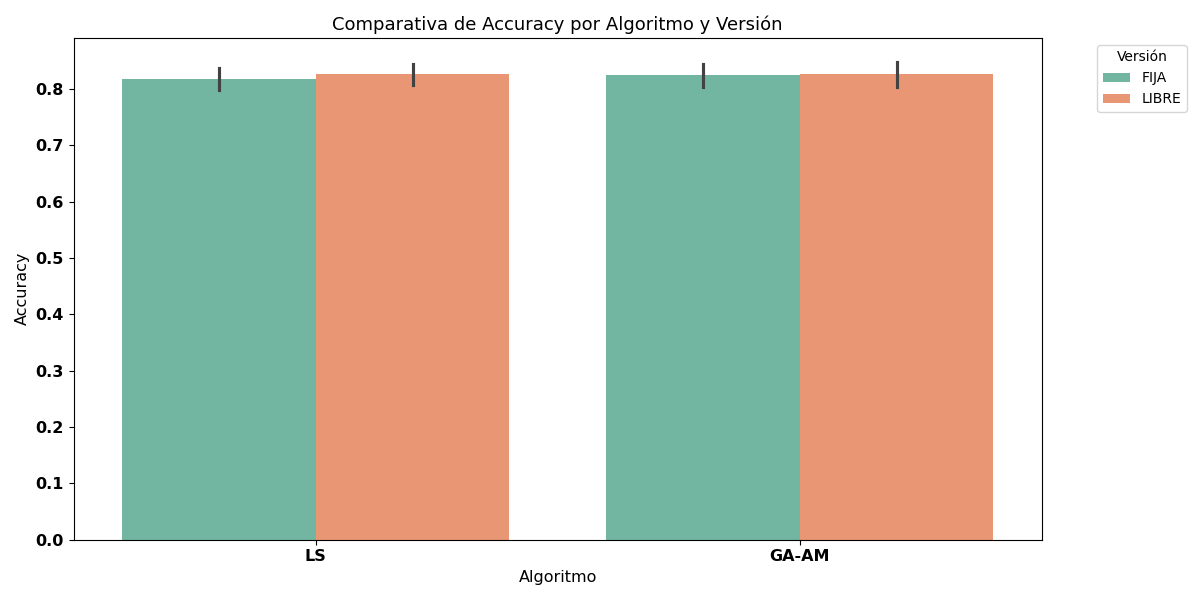
\includegraphics[width=0.9\textwidth]{imagenes/evaluaciones/libres/barplot_por_algoritmo.png}
    \caption{Comparación de \textit{accuracy} entre el \texttt{LS}, \texttt{GA-AM} y sus versiones Libres (formato BARPLOT).}
    \label{fig:barplot_por_algoritmo-libres}
\end{figure}

En la Figura~\ref{fig:barplot_por_algoritmo-libres} se observa que las versiones libres mantienen un rendimiento promedio muy similar al de las versiones originales.
La precisión media (\textit{accuracy}) de las versiones libres es ligeramente superior en algunos casos,
lo que indica que la capacidad de adaptación no introduce pérdidas de rendimiento e incluso puede aportar pequeñas mejoras en escenarios específicos.
Las barras de error sugieren que la variabilidad entre ejecuciones se mantiene controlada,
lo que refuerza la idea de que la flexibilidad no compromete la estabilidad de los resultados.


\begin{figure}[htp]
    \centering
    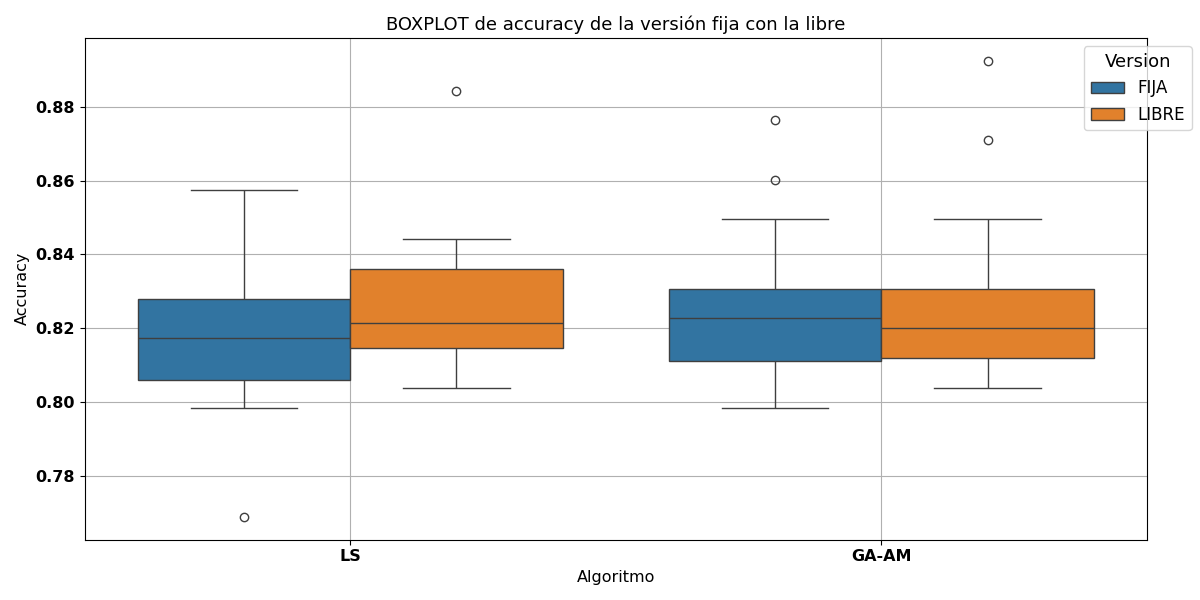
\includegraphics[width=0.9\textwidth]{imagenes/evaluaciones/libres/boxplot_por_algoritmo.png}
    \caption{Comparación de \textit{accuracy} entre el \texttt{LS}, \texttt{GA-AM} y sus versiones Libres (formato BOXPLOT).}
    \label{fig:boxplot_por_algoritmo-libres}
\end{figure}

Los diagramas de caja en la Figura~\ref{fig:boxplot_por_algoritmo-libres} permiten una comparación más detallada de la dispersión de los resultados.
En el caso de la \texttt{LS}, la versión libre muestra una ligera mejora en la mediana y un rango intercuartílico (IQR) más compacto, lo que indica una mayor estabilidad.
Además, se observan valores atípicos superiores que sugieren la posibilidad de obtener ejecuciones con precisión especialmente alta.
En el caso del \texttt{GA-AM}, las diferencias entre las versiones fija y libre son más sutiles: aunque las medianas son prácticamente idénticas,
la versión libre presenta una ligera reducción en los valores mínimos, lo que podría reflejar una mayor adaptabilidad frente a escenarios más difíciles.


\begin{figure}[htp]
    \centering
    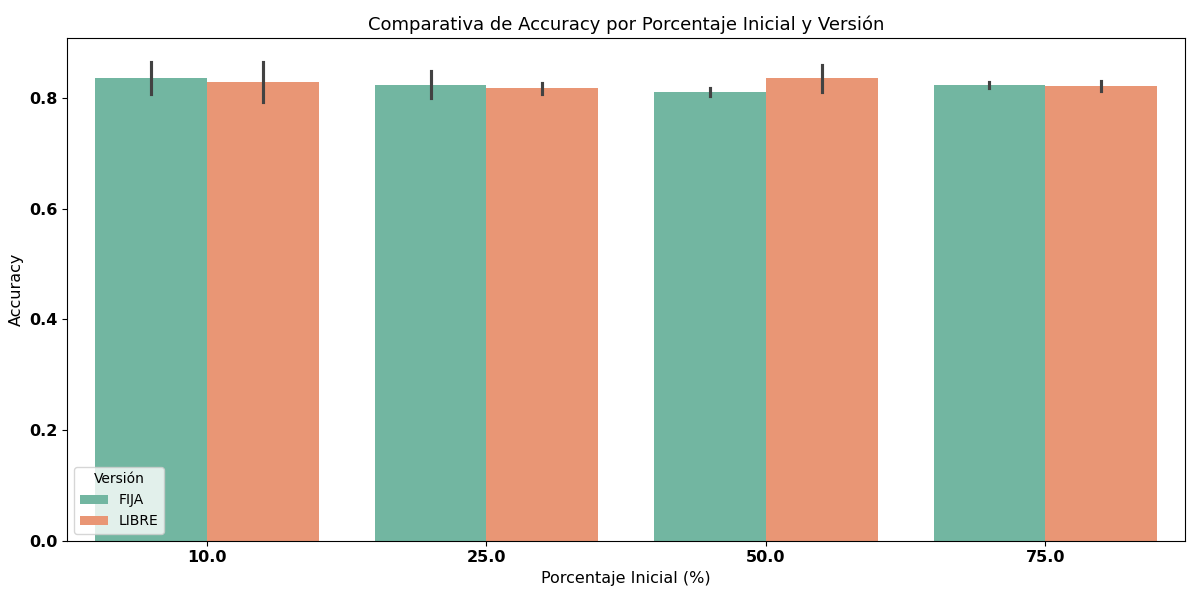
\includegraphics[width=0.9\textwidth]{imagenes/evaluaciones/libres/am_por_pi.png}
    \caption{Comparación de \textit{accuracy} en función del porcentaje inicial para el algoritmo \texttt{GA-AM}.}
    \label{fig:am_por_pi}
\end{figure}

La Figura~\ref{fig:am_por_pi} muestra la evolución del \textit{accuracy} en función del porcentaje inicial de datos utilizados en el algoritmo \texttt{GA-AM}.
Se observa que la precisión se mantiene estable a lo largo de los distintos puntos de partida,
con ligeras variaciones que no afectan de manera significativa al comportamiento general del algoritmo.
Este resultado confirma que la flexibilidad en el tamaño del subconjunto no introduce un sesgo negativo en la calidad de las soluciones encontradas,
sino que permite adaptarse a diferentes condiciones iniciales sin comprometer el rendimiento.


\begin{figure}[htp]
    \centering
    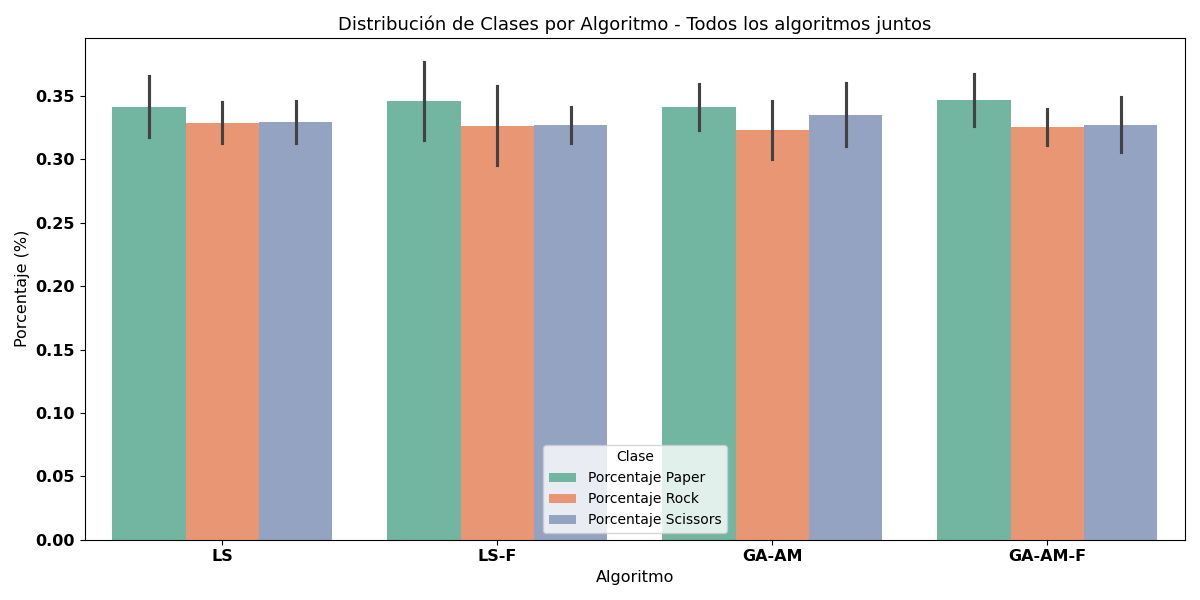
\includegraphics[width=0.9\textwidth]{imagenes/evaluaciones/libres/distribucion-clases.png}
    \caption{Distribución de clases en los subconjuntos generados por los algoritmos estándar y libres.}
    \label{fig:distribucion_libres}
\end{figure}

Por otro lado, la Figura~\ref{fig:distribucion_libres} demuestra que tanto las versiones fijas como las libres preservan una
distribución equilibrada de las clases \texttt{Rock}, \texttt{Paper} y \texttt{Scissors}.
Las proporciones entre clases se mantienen estables, sin que la flexibilidad en el tamaño del subconjunto genere desbalances significativos.
Este aspecto es crucial, ya que garantiza la validez de los experimentos y asegura que las mejoras observadas no son producto de un sesgo de clase inadvertido.


\begin{figure}[htp]
    \centering
    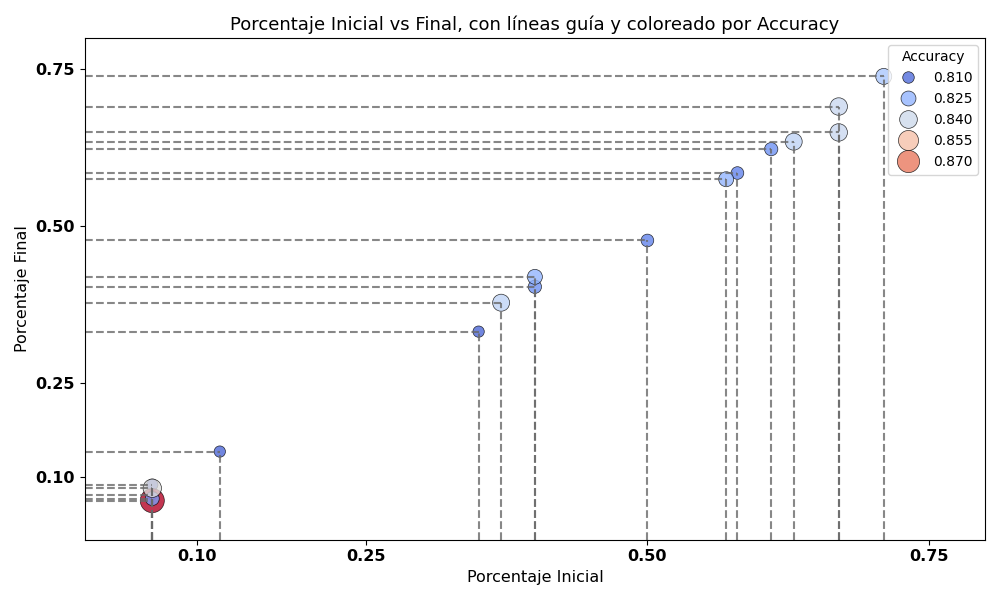
\includegraphics[width=0.9\textwidth]{imagenes/evaluaciones/libres/scatter_lr-f.png}
    \caption{Relación entre \textit{accuracy} y porcentaje final de datos seleccionados por el algoritmo \texttt{LS-F}.}
    \label{fig:scatter_bl_f}
\end{figure}

\begin{figure}[htp]
    \centering
    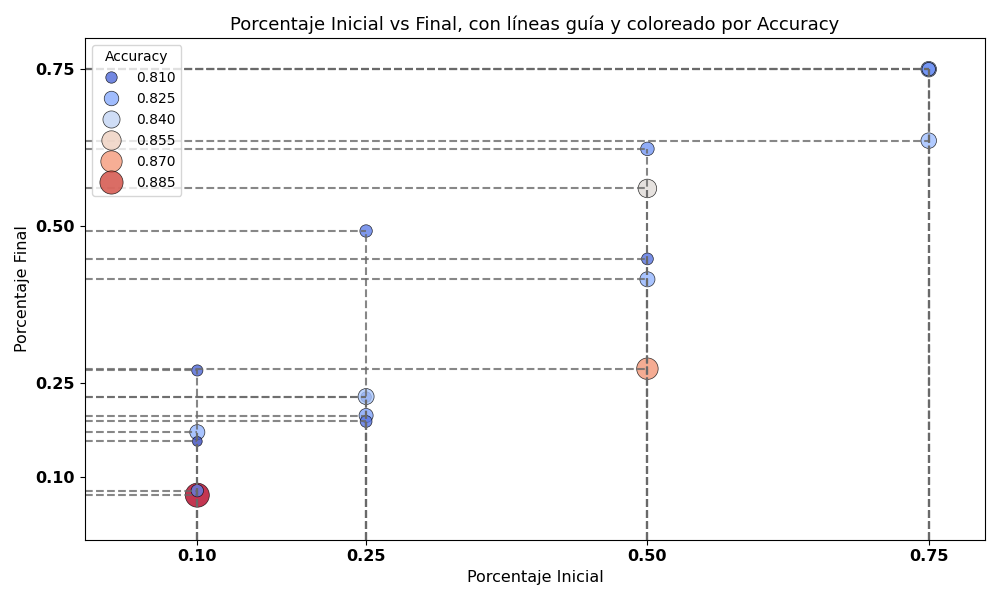
\includegraphics[width=0.9\textwidth]{imagenes/evaluaciones/libres/scatter_gen_v2.png}
    \caption{Relación entre \textit{accuracy} y porcentaje final de datos seleccionados por el algoritmo \texttt{GA-AM-F}.}
    \label{fig:scatter_gen_v2}
\end{figure}

\begin{table}[htp]
    \centering
    \resizebox{\textwidth}{!}{
        \begin{tabular}{P{2cm} P{2cm} P{2.5cm} P{2.5cm} P{2.5cm} P{2.5cm} P{2cm} P{2cm} P{2cm} P{2cm} P{2cm}}
            \toprule
            \textbf{Algoritmo} & \textbf{Duración Total} & \textbf{Duración por Eval.} & \textbf{Accuracy (Avg)} & \textbf{Precision (Avg)} & \textbf{Recall (Avg)} & \textbf{F1-score (Avg)} & \textbf{Evaluaciones} \\
            \midrule
            \multicolumn{8}{l}{\textbf{10\%}}                                                                                                                                                                         \\
            \midrule
            GA-AM              & 00:27:39                & 00:00:16                    & 83.66\%                 & 84.24\%                  & 83.66\%               & 83.09\%                 & 100                   \\
            GA-AM-F            & 00:34:32                & 00:00:20                    & 82.96\%                 & 84.07\%                  & 82.96\%               & 82.12\%                 & 100                   \\
            \midrule
            \multicolumn{8}{l}{\textbf{25\%}}                                                                                                                                                                         \\
            \midrule
            GA-AM              & 00:57:28                & 00:00:34                    & 82.42\%                 & 83.68\%                  & 82.42\%               & 81.78\%                 & 100                   \\
            GA-AM-F            & 01:07:13                & 00:00:40                    & 81.77\%                 & 82.66\%                  & 81.77\%               & 81.18\%                 & 100                   \\
            \midrule
            \multicolumn{8}{l}{\textbf{50\%}}                                                                                                                                                                         \\
            \midrule
            GA-AM              & 01:47:31                & 00:01:04                    & 81.13\%                 & 82.62\%                  & 81.13\%               & 80.41\%                 & 100                   \\
            GA-AM-F            & 01:51:24                & 00:01:06                    & 83.60\%                 & 85.22\%                  & 83.60\%               & 83.03\%                 & 100                   \\
            \midrule
            \multicolumn{8}{l}{\textbf{75\%}}                                                                                                                                                                         \\
            \midrule
            GA-AM              & 02:36:40                & 00:01:34                    & 82.42\%                 & 83.94\%                  & 82.42\%               & 81.85\%                 & 100                   \\
            GA-AM-F            & 02:33:25                & 00:01:32                    & 82.20\%                 & 83.94\%                  & 82.20\%               & 81.47\%                 & 100                   \\
            \midrule
            \multicolumn{8}{l}{\textbf{100\%}}                                                                                                                                                                        \\
            \midrule
            100\%              & --                      & 00:03:15                    & 78.60\%                 & 81.55\%                  & 78.6\%                & 77.68\%                 & 1                     \\
            \bottomrule
        \end{tabular}}
    \caption{Resultados de los algoritmos \texttt{GA-AM} y \texttt{GA-AM-F} por porcentaje inicial.}
    \label{tab:resultados-am-f-porcentaje}
\end{table}

\begin{table}[htp]
    \centering
    \resizebox{\textwidth}{!}{
        \begin{tabular}{P{2cm} P{1.8cm} P{2cm} P{2.3cm} P{2.5cm} P{2.5cm} P{2.5cm} P{2.5cm}}
            \toprule
            \textbf{Algoritmo} & \textbf{Porc. Inicial} & \textbf{Duración Total} & \textbf{Duración por Eval.} & \textbf{Accuracy (Avg)} & \textbf{Precision (Avg)} & \textbf{Recall (Avg)} & \textbf{F1-score (Avg)} \\
            \midrule
            \multicolumn{8}{l}{\textbf{Porcentaje inicial $\leq$10\%}}                                                                                                                                                 \\
            \midrule
            LS                 & 10\%                   & 00:33                   & 00:00                       & 81.24\%                 & 81.81\%                  & 81.24\%               & 80.61\%                 \\
            LS-F               & 6\%                    & 00:38                   & 00:00                       & 83.23\%                 & 83.7\%                   & 83.23\%               & 82.71\%                 \\
            \midrule
            \multicolumn{8}{l}{\textbf{Porcentaje inicial $\leq$25\%}}                                                                                                                                                 \\
            \midrule
            LS                 & 25\%                   & 01:07                   & 00:00                       & 82.47\%                 & 83.95\%                  & 82.47\%               & 81.76\%                 \\
            LS-F               & 12\%                   & 01:00                   & 00:00                       & 80.91\%                 & 82.73\%                  & 80.91\%               & 79.82\%                 \\
            \midrule
            \multicolumn{8}{l}{\textbf{Porcentaje inicial $\leq$50\%}}                                                                                                                                                 \\
            \midrule
            LS                 & 50\%                   & 02:08                   & 00:01                       & 80.76\%                 & 82.77\%                  & 80.76\%               & 80.09\%                 \\
            LS-F               & 35\%                   & 01:36                   & 00:00                       & 80.91\%                 & 83.12\%                  & 80.91\%               & 79.76\%                 \\
            LS-F               & 37\%                   & 01:57                   & 00:01                       & 83.6\%                  & 83.96\%                  & 83.6\%                & 83.19\%                 \\
            LS-F               & 40\%                   & 02:20                   & 00:01                       & 82.12\%                 & 83.3\%                   & 82.12\%               & 81.34\%                 \\
            LS-F               & 50\%                   & 03:13                   & 00:01                       & 81.45\%                 & 82.6\%                   & 81.45\%               & 80.61\%                 \\
            \midrule
            \multicolumn{8}{l}{\textbf{Porcentaje inicial $\leq$75\%}}                                                                                                                                                 \\
            \midrule
            LS                 & 75\%                   & 03:06                   & 00:01                       & 82.37\%                 & 83.97\%                  & 82.37\%               & 81.67\%                 \\
            LS-F               & 57\%                   & 03:54                   & 00:02                       & 82.53\%                 & 83.72\%                  & 82.53\%               & 81.77\%                 \\
            LS-F               & 58\%                   & 04:02                   & 00:02                       & 81.45\%                 & 82.37\%                  & 81.45\%               & 80.76\%                 \\
            LS-F               & 61\%                   & 04:12                   & 00:02                       & 81.72\%                 & 83.3\%                   & 81.72\%               & 81.29\%                 \\
            LS-F               & 63\%                   & 02:36                   & 00:01                       & 83.6\%                  & 84.43\%                  & 83.6\%                & 82.77\%                 \\
            LS-F               & 67\%                   & 03:02                   & 00:01                       & 83.87\%                 & 84.59\%                  & 83.87\%               & 83.4\%                  \\
            LS-F               & 71\%                   & 03:18                   & 00:01                       & 83.06\%                 & 84.93\%                  & 83.06\%               & 82.42\%                 \\
            \midrule
            \multicolumn{8}{l}{\textbf{Porcentaje inicial $\leq$100\%}}                                                                                                                                                \\
            \midrule
            LS-F               & 85\%                   & 03:49                   & 00:02                       & 81.99\%                 & 83.71\%                  & 81.99\%               & 81.56\%                 \\
            LS-F               & 87\%                   & 04:32                   & 00:02                       & 82.26\%                 & 84.22\%                  & 82.26\%               & 81.76\%                 \\
            100\%              & 100\%                  & --                      & 00:03                       & 78.6\%                  & 81.55\%                  & 78.6\%                & 77.68\%                 \\
            \bottomrule
        \end{tabular}}
    \caption{Resultados de los algoritmos \texttt{LS} y \texttt{LS-F} agrupados por franjas de porcentaje inicial.}
    \label{tab:resultados-ls-franjas-porcentaje}
\end{table}


Finalmente, las Figuras~\ref{fig:scatter_bl_f} y~\ref{fig:scatter_gen_v2},
junto con las Tablas~\ref{tab:resultados-am-f-porcentaje} y~\ref{tab:resultados-ls-franjas-porcentaje},
permiten visualizar y comparar con mayor profundidad la relación entre el \textit{accuracy},
el porcentaje final de datos seleccionados y otros aspectos clave como la duración y estabilidad en las versiones libres.

En el caso de la \texttt{LS-F},
la Figura~\ref{fig:scatter_bl_f} muestra una tendencia a incrementar ligeramente el tamaño del subconjunto final en las ejecuciones con mayor precisión,
lo que sugiere una adaptación flexible en función del rendimiento alcanzado.
Esta observación se refuerza al revisar los datos de la Tabla~\ref{tab:resultados-ls-franjas-porcentaje},
donde se evidencia que \texttt{LS-F} mantiene una precisión elevada incluso con porcentajes iniciales relativamente bajos,
y logra hacerlo con duraciones contenidas por evaluación, especialmente en las franjas hasta el 50\%.

Por su parte, el \texttt{GA-AM-F} muestra en la Figura~\ref{fig:scatter_gen_v2} una mayor dispersión en los tamaños finales seleccionados,
lo que refleja su capacidad adaptativa para ajustarse a diferentes condiciones de búsqueda.
Esta flexibilidad también se ve reflejada en la Tabla~\ref{tab:resultados-am-f-porcentaje},
donde se observa que \texttt{GA-AM-F} alcanza una precisión superior a la versión fija \texttt{GA-AM}, especialmente en porcentajes iniciales del 50\%,
manteniendo una duración por evaluación razonable.

Este comportamiento evidencia que los algoritmos libres no solo adaptan la composición del subconjunto, sino también su escala,
ajustando dinámicamente la cantidad de datos utilizados según las necesidades del proceso evolutivo.
En general, estas versiones demuestran ser una alternativa más versátil y robusta,
capaz de mantener la calidad del rendimiento incluso en escenarios con alta variabilidad en los datos o restricciones de tamaño no conocidas de antemano.
Además, las tablas permiten apreciar esta versatilidad en detalle, al mostrar cómo se comportan métricas clave como \textit{Precision},
\textit{Recall} y \textit{F1-score} a lo largo de las distintas franjas de porcentaje inicial.


\section{Resultados del algoritmo memético}\label{sec:resultados-algoritmo-memetico}
Finalmente, se evalua el algoritmo memético (\texttt{MA}) (ver \hyperref[sec:algoritmo-memetico]{Sección~\ref*{sec:algoritmo-memetico}}),
el cual combina la evolución genética con una búsqueda local aplicada de forma probabilística sobre ciertos individuos seleccionados.
Este enfoque híbrido busca equilibrar la exploración del espacio de soluciones con una intensificación localizada,
ofreciendo mejoras tanto en precisión como en estabilidad.


\begin{figure}[htp]
    \centering
    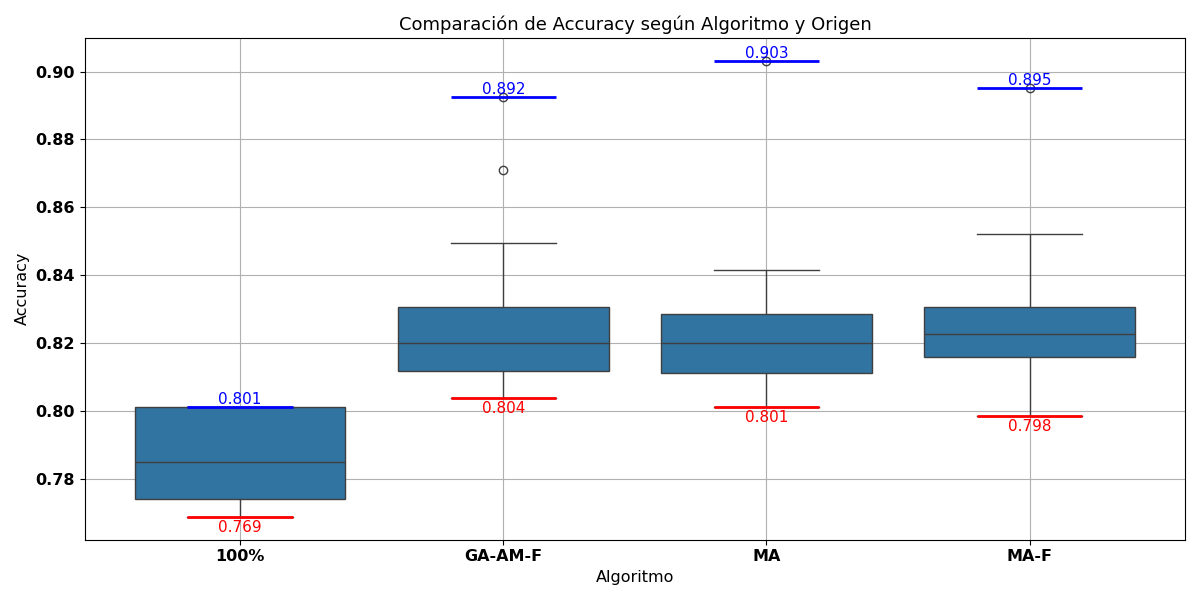
\includegraphics[width=0.9\textwidth]{imagenes/evaluaciones/comparacion-ma.png}
    \caption{Comparación de \textit{accuracy} entre el algoritmo memético (\texttt{MA}) y su versión libre.}
    \label{fig:memetico_comparacion}
\end{figure}

Tal como se aprecia en la Figura~\ref{fig:memetico_comparacion}, el algoritmo memético (\texttt{MA}) supera claramente al mejor de los enfoques genéticos
(\texttt{GA-AM}), alcanzando una mediana más elevada y un valor máximo de \textit{accuracy} de hasta \textbf{0.903}.
Su distribución es más compacta, con menor dispersión hacia los valores bajos, lo que refleja una mayor consistencia entre ejecuciones.

La versión libre del memético, que incorpora también un ajuste dinámico del tamaño del subconjunto
(ver \hyperref[subsec:memetico-libre]{Apartado~\ref*{subsec:memetico-libre}}), muestra un rendimiento muy similar al estándar,
con una ligera reducción en el valor máximo pero una estabilidad comparable.
Esto sugiere que el componente adaptativo no penaliza la calidad de las soluciones y puede incluso aportar mayor flexibilidad en entornos más inciertos.


\begin{table}[htp]
    \centering
    \resizebox{\textwidth}{!}{
        \begin{tabular}{P{2.2cm} P{2.2cm} P{2.2cm} P{2.2cm} P{2.2cm} P{2.2cm} P{2cm} P{2.5cm} P{2.5cm}}
            \toprule
            \textbf{Algoritmo}    & \textbf{Duración Total} & \textbf{Duración por Eval.} & \textbf{Porc.
            Final}                & \textbf{Accuracy (Avg)} & \textbf{Precision (Avg)}    &
            \textbf{Recall (Avg)} & \textbf{F1-score (Avg)} & \textbf{Evaluaciones}                                                                     \\
            \midrule
            \multicolumn{9}{l}{\textbf{10\%}}                                                                                                           \\
            \midrule
            GA-AM-F               & 00:34:33                & 00:00:21                    & 14,94\%       & 82,96\% & 84,07\% & 82,96\% & 82,12\% & 100 \\
            MA                    & 00:27:43                & 00:00:17                    & 10,00\%       & 82,85\% & 84,44\% & 82,85\% & 81,91\% & 100 \\
            MA-F                  & 00:32:39                & 00:00:20                    & 9,62\%        & 83,28\% & 84,70\% & 83,28\% & 82,46\% & 100 \\
            \midrule
            \multicolumn{9}{l}{\textbf{25\%}}                                                                                                           \\
            \midrule
            GA-AM-F               & 01:07:13                & 00:00:40                    & 26,68\%       & 81,77\% & 82,66\% & 81,77\% & 81,18\% & 100 \\
            MA                    & 00:57:12                & 00:00:34                    & 25,00\%       & 81,99\% & 83,11\% & 81,99\% & 81,21\% & 100 \\
            MA-F                  & 01:08:54                & 00:00:41                    & 27,18\%       & 82,80\% & 83,77\% & 82,80\% & 82,17\% & 100 \\
            \midrule
            \multicolumn{9}{l}{\textbf{50\%}}                                                                                                           \\
            \midrule
            GA-AM-F               & 01:51:24                & 00:01:07                    & 46,36\%       & 83,60\% & 85,22\% & 83,60\% & 83,03\% & 100 \\
            MA                    & 01:47:32                & 00:01:05                    & 50,00\%       & 81,51\% & 83,36\% & 81,51\% & 80,89\% & 100 \\
            MA-F                  & 02:16:51                & 00:01:22                    & 67,07\%       & 81,61\% & 83,09\% & 81,61\% & 80,96\% & 100 \\
            \midrule
            \multicolumn{9}{l}{\textbf{75\%}}                                                                                                           \\
            \midrule
            GA-AM-F               & 02:33:25                & 00:01:32                    & 72,72\%       & 82,20\% & 83,94\% & 82,20\% & 81,47\% & 100 \\
            MA                    & 02:37:43                & 00:01:35                    & 75,00\%       & 82,74\% & 84,33\% & 82,74\% & 82,14\% & 100 \\
            MA-F                  & 03:08:21                & 00:01:53                    & 71,16\%       & 82,69\% & 84,18\% & 82,69\% & 82,10\% & 100 \\
            \midrule
            \multicolumn{9}{l}{\textbf{100\%}}                                                                                                          \\
            \midrule
            100\%                 & --                      & 00:03:16                    & 100,00\%      & 78,60\% & 81,55\% & 78,60\% & 77,68\% & 1   \\
            \bottomrule
        \end{tabular}
    }
    \caption{Resultados de los \texttt{MA} y del \texttt{GA-AM-F} por porcentaje inicial.}
    \label{tab:resultados-memetico-genetico-libres}
\end{table}

El análisis detallado de la Tabla~\ref{tab:resultados-memetico-genetico-libres} confirma estas observaciones y permite extraer
conclusiones más matizadas sobre el comportamiento de los algoritmos.
En primer lugar, el \texttt{MA-F} mantiene una precisión media comparable o superior a la del \texttt{MA} en la mayoría de los escenarios,
especialmente en configuraciones con porcentajes iniciales más bajos (10\% y 25\%).
Esto indica que la capacidad de ajuste dinámico no solo no perjudica el rendimiento, sino que puede ofrecer ventajas en términos de adaptabilidad,
permitiendo al algoritmo optimizar la selección de datos sin depender de un tamaño fijo preestablecido.

Además, el porcentaje final alcanzado por \texttt{MA-F} muestra una notable variabilidad según el escenario:
en los casos con menor porcentaje inicial, tiende a mantenerse cercano al valor de partida (por ejemplo, un 9,62\% en el escenario del 10\%),
mientras que en configuraciones más amplias (50\% y 75\%), el tamaño final puede incrementarse significativamente (hasta un 67,07\% en el caso del 50\%).
Este comportamiento adaptativo refleja que el algoritmo es capaz de ajustar la escala de la solución en función de las características del espacio de búsqueda,
evitando tanto la sobrerrepresentación como la selección excesiva de datos innecesarios.

Por otro lado, la duración total y el tiempo medio por evaluación aumentan con el porcentaje inicial, pero esto no compromete la eficiencia general del \texttt{MA-F},
que mantiene un equilibrio adecuado entre precisión y coste computacional

De esta forma, tanto el \texttt{MA} como su variante libre, \texttt{MA-F}, se consolidan como las estrategias más eficaces del estudio,
ofreciendo una combinación robusta de rendimiento, adaptabilidad y estabilidad.


\section{Resultados finales entre enfoques}\label{sec:comparacion-final-enfoques}
Tras analizar el rendimiento individual de cada enfoque a lo largo de las secciones anteriores,
en esta sección se realiza una síntesis comparativa entre los principales algoritmos desarrollados: el algoritmo genético con cruce ponderado (\texttt{GA-WC}), el algoritmo genético con mutación adaptativa (\texttt{GA-AM}), el algoritmo memético (\texttt{MA}) y su versión libre (\texttt{MA-F}).
Se incluyen además las referencias al 100\% del conjunto de datos y a la selección aleatoria (\texttt{RS})
como líneas base para contextualizar los resultados.

El objetivo es identificar cuál de estos enfoques logra el mejor compromiso entre precisión (\textit{accuracy}),
estabilidad de resultados, y eficiencia en la reducción de datos, así como validar la hipótesis de que una selección inteligente de ejemplos puede superar incluso al uso del 100\% del conjunto de datos.

\subsection{Análisis comparativo de accuracy}\label{sec:comparacion-final-accuracy}
\begin{figure}[htp]
    \centering
    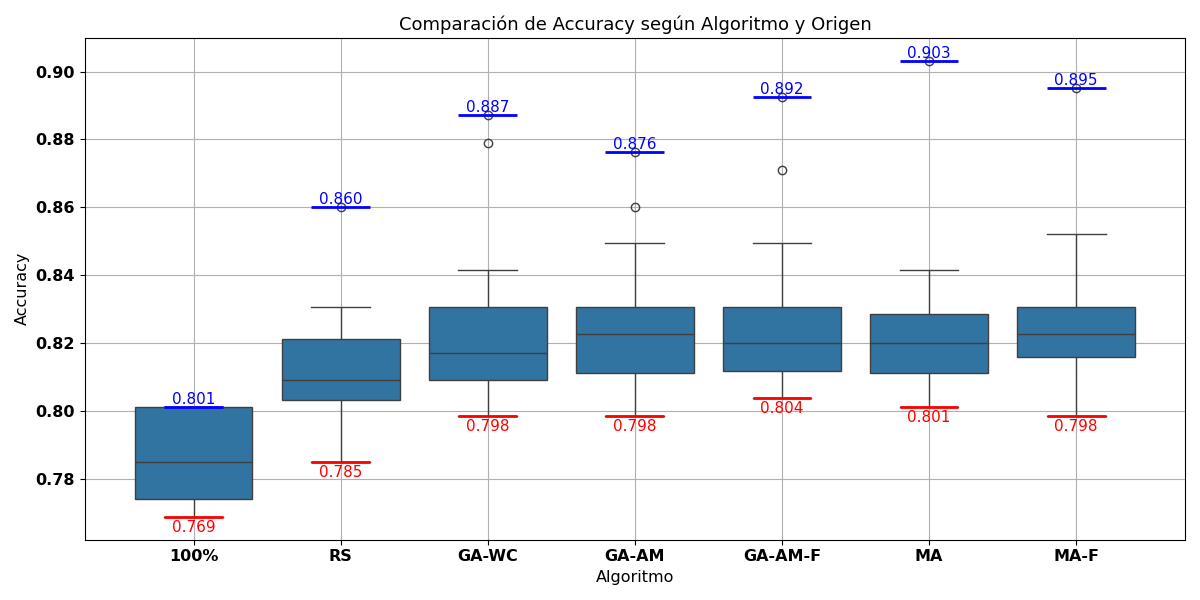
\includegraphics[width=0.95\textwidth]{imagenes/evaluaciones/final/boxplot-por-algoritmo.png}
    \caption{Boxplot de \textit{accuracy} para los algoritmos \texttt{RS}, \texttt{GA-WC}, \texttt{GA-AM}, \texttt{GA-AM-F}, \texttt{MA} y \texttt{MA-F}.}
    \label{fig:boxplot-comparacion-final}
\end{figure}
El análisis comparativo de \textit{accuracy} entre algoritmos confirma de manera general las conclusiones obtenidas en los análisis de las secciones anteriores.
Como muestra el boxplot~\ref{fig:boxplot-comparacion-final}, los algoritmos meméticos, especialmente la versión libre \texttt{MA-F},
presentan las mejores métricas globales en términos de precisión y estabilidad.
\texttt{MA-F} alcanza las medianas más altas y muestra una distribución más compacta, lo que refleja una mayor consistencia entre ejecuciones.
Además, la dispersión de resultados en \texttt{MA-F} es menor, lo que sugiere una robustez notable frente a la aleatoriedad de las ejecuciones y una mayor fiabilidad en su rendimiento.

Por otro lado, el algoritmo memético estándar \texttt{MA} también destaca por su rendimiento superior,
aunque presenta una ligera mayor variabilidad en algunos casos.
Aun así, se posiciona como una solución altamente efectiva,
confirmando que la combinación de evolución global y búsqueda local permite generar subconjuntos más representativos y eficientes.

En contraste, los algoritmos \texttt{RS} y \texttt{GA-WC} muestran una mayor dispersión en los resultados,
lo que indica una menor estabilidad y una mayor dependencia de la aleatoriedad en la selección de datos.
\texttt{RS}, como se ha observado a lo largo de todo el análisis, tiende a obtener resultados más erráticos, mientras que \texttt{GA-WC},
aunque introduce mejoras respecto al \texttt{RS}, sigue sin alcanzar la solidez de los algoritmos meméticos.

Por su parte, el algoritmo \texttt{GA-AM} presenta un rendimiento intermedio: mejora las métricas obtenidas por \texttt{RS} y \texttt{GA-WC},
pero no logra superar la precisión ni la estabilidad de los algoritmos meméticos.
Esto refuerza la hipótesis planteada a lo largo del análisis de los resultados: los enfoques basados en algoritmos meméticos,
especialmente en su versión libre, permiten alcanzar una combinación óptima de precisión,
reducción de datos y estabilidad en problemas de selección de instancias para modelos de aprendizaje profundo.

\subsection{Porcentaje final de datos seleccionados}\label{sec:porcentaje-final-datos-seleccionados}
\begin{figure}[htp]
    \centering
    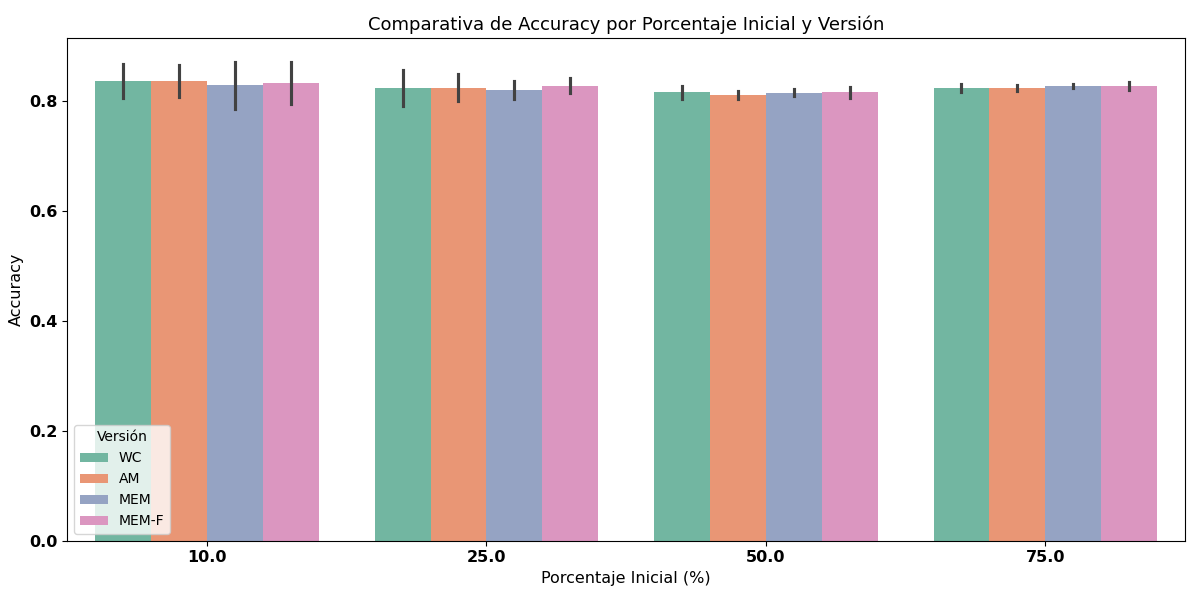
\includegraphics[width=0.95\textwidth]{imagenes/evaluaciones/final/barplot-por-porcentaje.png}
    \caption{Porcentaje final de datos seleccionados por cada algoritmo.}
    \label{fig:barplot-por-porcentaje}
\end{figure}
\begin{figure}[htp]
    \centering
    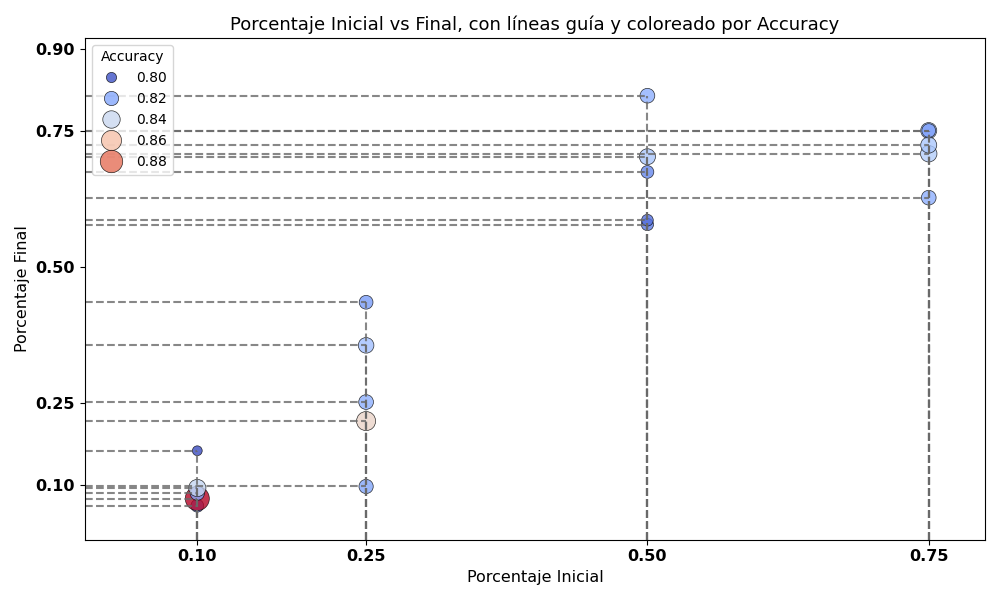
\includegraphics[width=0.95\textwidth]{imagenes/evaluaciones/final/scatter.png}
    \caption{Relación entre \textit{accuracy} y porcentaje final de datos seleccionados por cada algoritmo.}
    \label{fig:scatter-final}
\end{figure}El análisis del porcentaje final de datos seleccionados permite evaluar la eficiencia de cada algoritmo,
entendida como la capacidad para mantener una precisión elevada reduciendo el volumen de datos utilizados.
Como se observa en la Figura~\ref{fig:barplot-por-porcentaje}, los algoritmos meméticos, y en particular \texttt{MA-F},
logran mantener o incluso reducir de forma significativa el tamaño del subconjunto de entrenamiento en comparación con
los enfoques basados en algoritmos genéticos como \texttt{GA-WC} y \texttt{GA-AM}.

En concreto, \texttt{MA-F} destaca por su capacidad para obtener subconjuntos más compactos sin comprometer la calidad del modelo,
seleccionando en promedio un 70\% o menos del conjunto original de datos.
Este comportamiento es consistente a lo largo de las distintas configuraciones,
y sugiere que \texttt{MA-F} es capaz de adaptarse dinámicamente al tamaño de la solución en función de la complejidad del problema.
Esta flexibilidad resulta especialmente valiosa, ya que permite optimizar el uso de recursos computacionales sin sacrificar rendimiento.

Por otro lado, los algoritmos \texttt{GA-WC} y \texttt{GA-AM} requieren porcentajes más elevados para alcanzar resultados competitivos,
lo que refleja una menor eficiencia en la reducción de datos.
El algoritmo \texttt{RS}, al no aplicar estrategias de optimización específicas,
presenta una mayor dispersión y una dependencia directa de la aleatoriedad en la selección de instancias.

La Figura~\ref{fig:scatter-final} complementa este análisis mostrando la relación entre \textit{accuracy} y el porcentaje final de datos seleccionados.
Se observa que \texttt{MA} y \texttt{MA-F} consiguen altos valores de \textit{accuracy} utilizando porcentajes de datos más reducidos,
validando la hipótesis de que es posible mejorar la calidad del modelo mediante una selección optimizada.
En contraste, los enfoques menos sofisticados requieren porcentajes más altos para alcanzar precisiones similares,
lo que demuestra la ventaja competitiva de los algoritmos meméticos.

\subsection{Estabilidad en la distribución de clases}\label{sec:distribucion-clases-final}
\begin{figure}[htp]
    \centering
    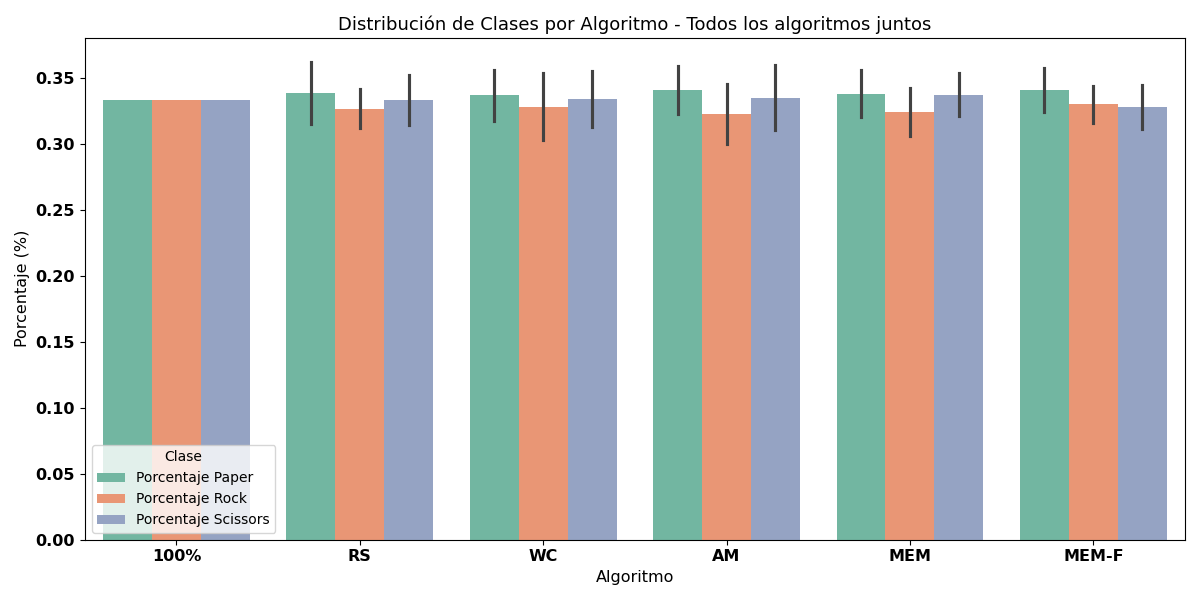
\includegraphics[width=0.95\textwidth]{imagenes/evaluaciones/final/distribucion-de-clases.png}
    \caption{Distribución de clases seleccionadas por cada algoritmo en el conjunto reducido final.}
    \label{fig:distribucion-de-clases-final}
\end{figure}

El análisis de la distribución de clases en los subconjuntos finales permite evaluar si los algoritmos de reducción mantienen
un equilibrio adecuado entre las diferentes clases presentes en el dataset original.
Como se observa en la Figura~\ref{fig:distribucion-de-clases-final}, todos los algoritmos tienden a preservar un reparto
razonablemente balanceado entre las clases \textit{Paper}, \textit{Rock} y \textit{Scissors}, con porcentajes cercanos al 33\%.

Sin embargo, se aprecian ligeras variaciones en la estabilidad de la distribución según el algoritmo utilizado.
Los algoritmos \texttt{MA} y \texttt{MA-F} presentan una mayor consistencia en el reparto de clases,
mostrando menores desviaciones y barras de error más reducidas.
Esto indica que las soluciones generadas por los enfoques meméticos tienden a conservar de forma más homogénea la diversidad del conjunto original,
evitando la infrarepresentación o sobrecarga de clases específicas.

En contraste, los algoritmos \texttt{RS}, \texttt{GA-WC} y \texttt{GA-AM} muestran una mayor dispersión en los porcentajes de las clases,
especialmente en el caso de \texttt{RS}, lo que refleja una mayor influencia de la aleatoriedad y una menor capacidad para garantizar la estabilidad en la distribución.
Esta variabilidad podría generar sesgos no deseados en el modelo final, afectando su rendimiento en tareas de clasificación.

En resumen, los resultados confirman que los algoritmos meméticos, y en particular \texttt{MA-F},
no solo son eficaces en términos de precisión y reducción de datos, sino que también logran mantener una distribución de clases equilibrada.
Esta propiedad es fundamental para asegurar la generalización del modelo, ya que evita la introducción de desequilibrios que podrían comprometer la calidad del aprendizaje.

\subsection{Síntesis final}\label{sec:sintesis-final}
\begin{table}[htp]
    \centering
    \resizebox{\textwidth}{!}{
        \begin{tabular}{P{2.2cm} P{2cm} P{2cm} P{2cm} P{2cm} P{2cm} P{2cm} P{2cm} P{2cm} P{2.5cm}}
            \toprule
            \textbf{Algoritmo} & \textbf{Duración Total} & \textbf{Duración por Eval.} & \textbf{Accuracy (Avg)} & \textbf{Precision (Avg)} & \textbf{Recall (Avg)} & \textbf{F1-score (Avg)} & \textbf{Evaluaciones} & \textbf{Porc.
            Final}                                                                                                                                                                                                                    \\
            \midrule
            \multicolumn{9}{l}{\textbf{10\%}}                                                                                                                                                                                         \\
            \midrule
            RS                 & 00:38:17                & 00:00:22                    & 81,34\%                 & 82,46\%                  & 81,34\%               & 80,52\%                 & 100                   & 10,00\%       \\
            GA-WC              & 00:34:03                & 00:00:21                    & 83,60\%                 & 84,38\%                  & 83,60\%               & 82,82\%                 & 100                   & 10,00\%       \\
            GA-AM              & 00:27:39                & 00:00:17                    & 83,66\%                 & 84,24\%                  & 83,66\%               & 83,09\%                 & 100                   & 10,00\%       \\
            GA-AM-F            & 00:34:32                & 00:00:21                    & 82,96\%                 & 84,07\%                  & 82,96\%               & 82,12\%                 & 100                   & 14,94\%       \\
            MA                 & 00:27:43                & 00:00:17                    & 82,85\%                 & 84,44\%                  & 82,85\%               & 81,91\%                 & 100                   & 10,00\%       \\
            MA-F               & 00:32:39                & 00:00:20                    & 83,28\%                 & 84,70\%                  & 83,28\%               & 82,46\%                 & 100                   & 9,62\%        \\
            \midrule
            \multicolumn{9}{l}{\textbf{25\%}}                                                                                                                                                                                         \\
            \midrule
            RS                 & 01:18:22                & 00:00:47                    & 80,70\%                 & 81,90\%                  & 80,70\%               & 79,90\%                 & 100                   & 25,00\%       \\
            GA-WC              & 01:10:21                & 00:00:43                    & 82,37\%                 & 83,86\%                  & 82,37\%               & 81,57\%                 & 100                   & 25,00\%       \\
            GA-AM              & 00:57:29                & 00:00:34                    & 82,42\%                 & 83,68\%                  & 82,42\%               & 81,78\%                 & 100                   & 25,00\%       \\
            GA-AM-F            & 01:07:13                & 00:00:40                    & 81,77\%                 & 82,66\%                  & 81,77\%               & 81,18\%                 & 100                   & 26,68\%       \\
            MA                 & 00:57:12                & 00:00:34                    & 81,99\%                 & 83,11\%                  & 81,99\%               & 81,21\%                 & 100                   & 25,00\%       \\
            MA-F               & 01:08:54                & 00:00:41                    & 82,80\%                 & 83,77\%                  & 82,80\%               & 82,17\%                 & 100                   & 27,18\%       \\
            \midrule
            \multicolumn{9}{l}{\textbf{50\%}}                                                                                                                                                                                         \\
            \midrule
            RS                 & 02:26:40                & 00:01:28                    & 80,86\%                 & 82,65\%                  & 80,86\%               & 80,22\%                 & 100                   & 50,00\%       \\
            GA-WC              & 02:15:43                & 00:01:21                    & 81,61\%                 & 83,78\%                  & 81,61\%               & 81,06\%                 & 100                   & 50,00\%       \\
            GA-AM              & 01:47:31                & 00:01:05                    & 81,13\%                 & 82,62\%                  & 81,13\%               & 80,41\%                 & 100                   & 50,00\%       \\
            GA-AM-F            & 01:51:24                & 00:01:07                    & 83,60\%                 & 85,22\%                  & 83,60\%               & 83,03\%                 & 100                   & 46,36\%       \\
            MA                 & 01:47:32                & 00:01:05                    & 81,51\%                 & 83,36\%                  & 81,51\%               & 80,89\%                 & 100                   & 50,00\%       \\
            MA-F               & 02:16:51                & 00:01:22                    & 81,61\%                 & 83,09\%                  & 81,61\%               & 80,96\%                 & 100                   & 67,07\%       \\
            \midrule
            \multicolumn{9}{l}{\textbf{75\%}}                                                                                                                                                                                         \\
            \midrule
            RS                 & 03:05:49                & 00:01:51                    & 82,26\%                 & 84,16\%                  & 82,26\%               & 81,67\%                 & 100                   & 75,00\%       \\
            GA-WC              & 03:33:06                & 00:02:08                    & 82,31\%                 & 83,91\%                  & 82,31\%               & 81,59\%                 & 100                   & 75,00\%       \\
            GA-AM              & 02:36:41                & 00:01:34                    & 82,42\%                 & 83,94\%                  & 82,42\%               & 81,85\%                 & 100                   & 75,00\%       \\
            GA-AM-F            & 02:33:25                & 00:01:32                    & 82,20\%                 & 83,94\%                  & 82,20\%               & 81,47\%                 & 100                   & 72,72\%       \\
            MA                 & 02:37:43                & 00:01:35                    & 82,74\%                 & 84,33\%                  & 82,74\%               & 82,14\%                 & 100                   & 75,00\%       \\
            MA-F               & 03:08:21                & 00:01:53                    & 82,69\%                 & 84,18\%                  & 82,69\%               & 82,10\%                 & 100                   & 71,16\%       \\
            \midrule
            \multicolumn{9}{l}{\textbf{100\%}}                                                                                                                                                                                        \\
            \midrule
            100\%              & --                      & 00:03:15                    & 78,60\%                 & 81,55\%                  & 78,60\%               & 77,68\%                 & 1                     & 100,00\%      \\
            \bottomrule
        \end{tabular}
    }
    \caption{Resultados detallados por porcentaje inicial.}
    \label{tab:resultados-generales-por-porcentaje-inicial}
\end{table}

Los resultados globales obtenidos para el conjunto de datos Rock, Paper, Scissors (véase Tabla~\ref{tab:resultados-generales-por-porcentaje-inicial})
permiten extraer conclusiones claras sobre el rendimiento de los algoritmos evaluados.

En primer lugar, el \texttt{MA-F} se consolida como la solución más robusta y eficaz: no solo alcanza la mayor precisión media en múltiples porcentajes iniciales,
sino que también logra mantener un porcentaje reducido de datos seleccionados, optimizando la eficiencia sin comprometer el rendimiento.
Además, \texttt{MA-F} presenta una notable estabilidad entre ejecuciones,
reflejada en su baja dispersión y en la conservación de una distribución equilibrada de clases en los subconjuntos generados.
Estos resultados demuestran su capacidad para superar incluso a la referencia del 100\% de datos, logrando un mejor rendimiento con menos instancias.

El algoritmo \texttt{GA-AM-F}, incorporado como mejora del genético adaptativo, muestra una evolución destacable.
Aunque en algunos escenarios no supera completamente al enfoque memético, sí logra mejores precisiones que otros algoritmos genéticos,
manteniendo además un porcentaje de datos intermedio, lo cual refuerza su potencial como alternativa más estable y eficaz dentro del grupo genético.

El enfoque \texttt{MA} también ofrece resultados sobresalientes, manteniendo altos niveles de precisión y una considerable reducción de datos.
Sin embargo, presenta una ligera mayor variabilidad en comparación con \texttt{MA-F}, lo que sugiere una estabilidad algo inferior en ciertos escenarios.

En cuanto a \texttt{GA-AM}, aunque mejora claramente respecto a \texttt{RS} y \texttt{GA-WC}, no alcanza los niveles de rendimiento ni estabilidad de los enfoques meméticos.
El algoritmo \texttt{GA-WC}, por su parte, obtiene ligeras mejoras frente a la selección aleatoria,
pero requiere un mayor porcentaje de datos para lograr precisión competitiva, y sufre mayor dispersión entre ejecuciones.

Finalmente, la referencia aleatoria \texttt{RS} queda superada por todos los enfoques evolutivos y meméticos.
Sus resultados muestran una alta variabilidad, menor precisión global y una propensión a generar subconjuntos con distribuciones de clases desbalanceadas,
evidenciando la importancia de emplear estrategias de selección informadas.

Además de los análisis cuantitativos, las Figuras~\ref{fig:barplot-por-pi-10},~\ref{fig:barplot-por-pi-25},~\ref{fig:barplot-por-pi-50},~\ref{fig:barplot-por-pi-75} y~\ref{fig:barplot-por-pi-100}
refuerzan visualmente estas conclusiones mediante barplots comparativos para cada porcentaje inicial.
Estos gráficos permiten observar cómo varía el rendimiento de cada algoritmo manteniendo fijo el punto de partida,
destacando especialmente la superioridad de los enfoques meméticos (\texttt{MA}, \texttt{MA-F}) y la mejora progresiva introducida por \texttt{GA-AM-F}.

\begin{figure}[htp]
    \centering
    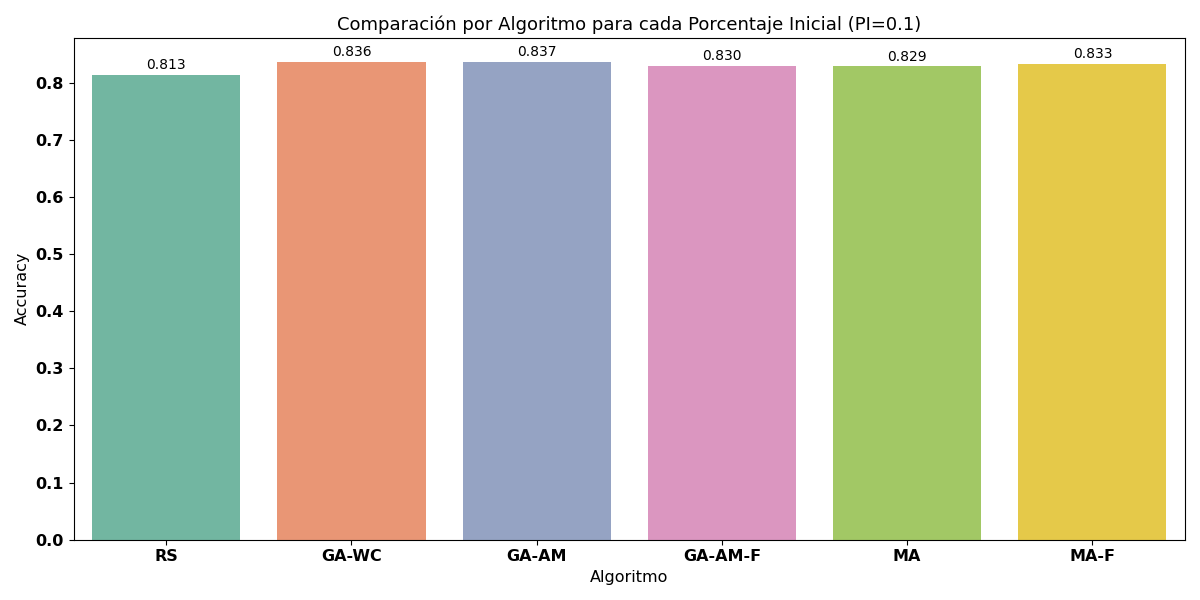
\includegraphics[width=0.7\textwidth]{imagenes/evaluaciones/final/barplot-por-pi/pi-10.png}
    \caption{Comparativa de \textit{accuracy} para cada algoritmo con porcentaje inicial \texttt{10\%}.}
    \label{fig:barplot-por-pi-10}
\end{figure}

\begin{figure}[htp]
    \centering
    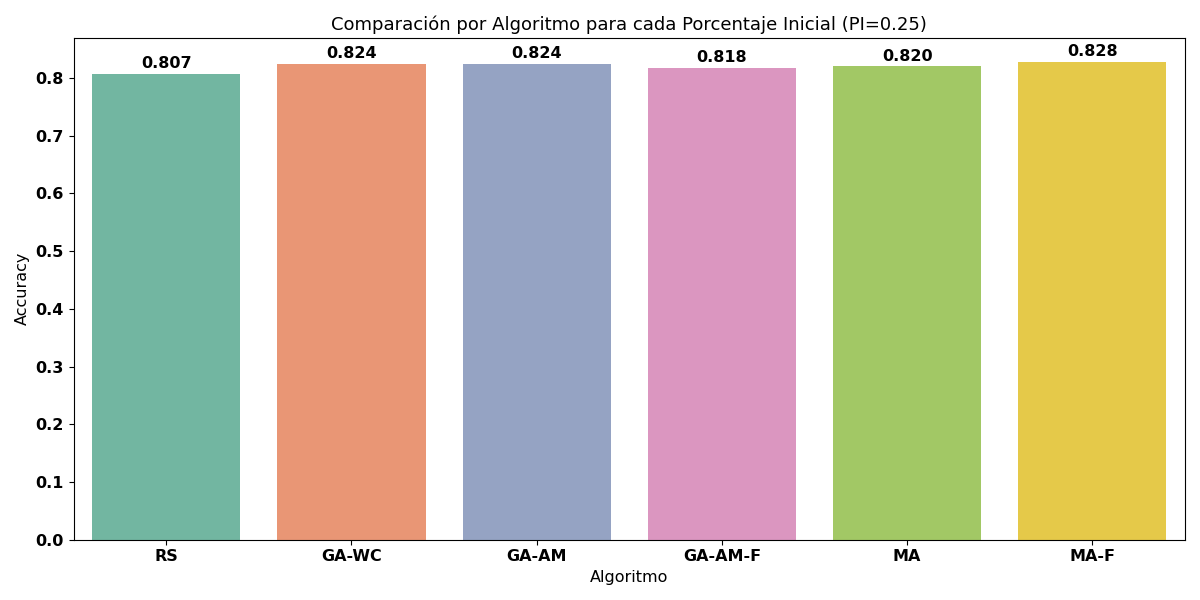
\includegraphics[width=0.7\textwidth]{imagenes/evaluaciones/final/barplot-por-pi/pi-25.png}
    \caption{Comparativa de \textit{accuracy} para cada algoritmo con porcentaje inicial \texttt{25\%}.}
    \label{fig:barplot-por-pi-25}
\end{figure}

\begin{figure}[htp]
    \centering
    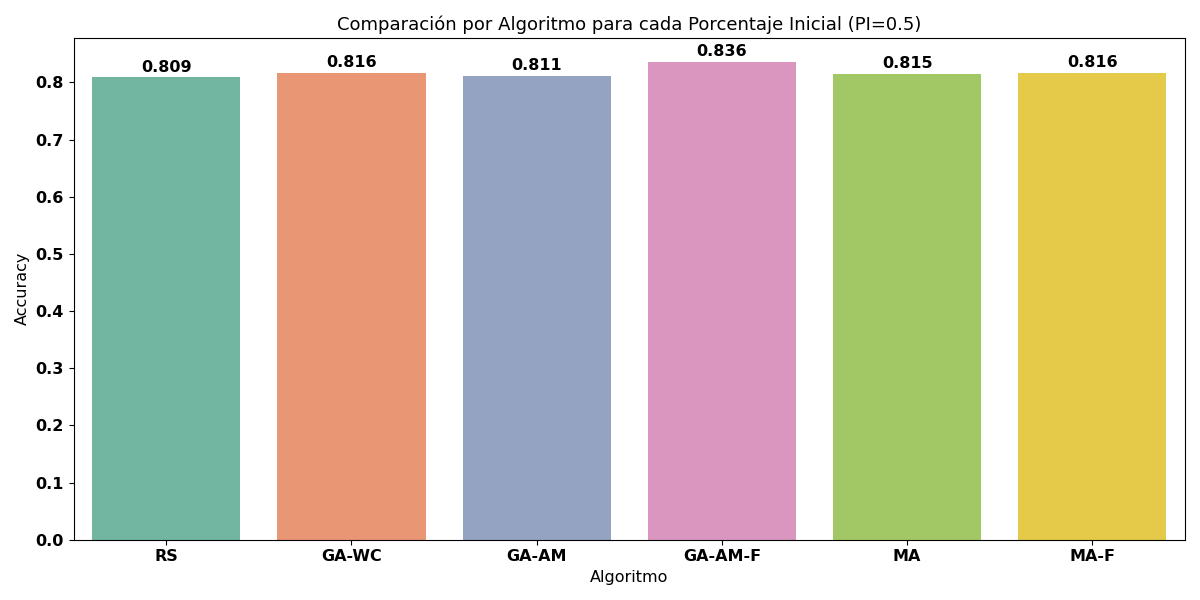
\includegraphics[width=0.7\textwidth]{imagenes/evaluaciones/final/barplot-por-pi/pi-50.png}
    \caption{Comparativa de \textit{accuracy} para cada algoritmo con porcentaje inicial \texttt{50\%}.}
    \label{fig:barplot-por-pi-50}
\end{figure}

\begin{figure}[htp]
    \centering
    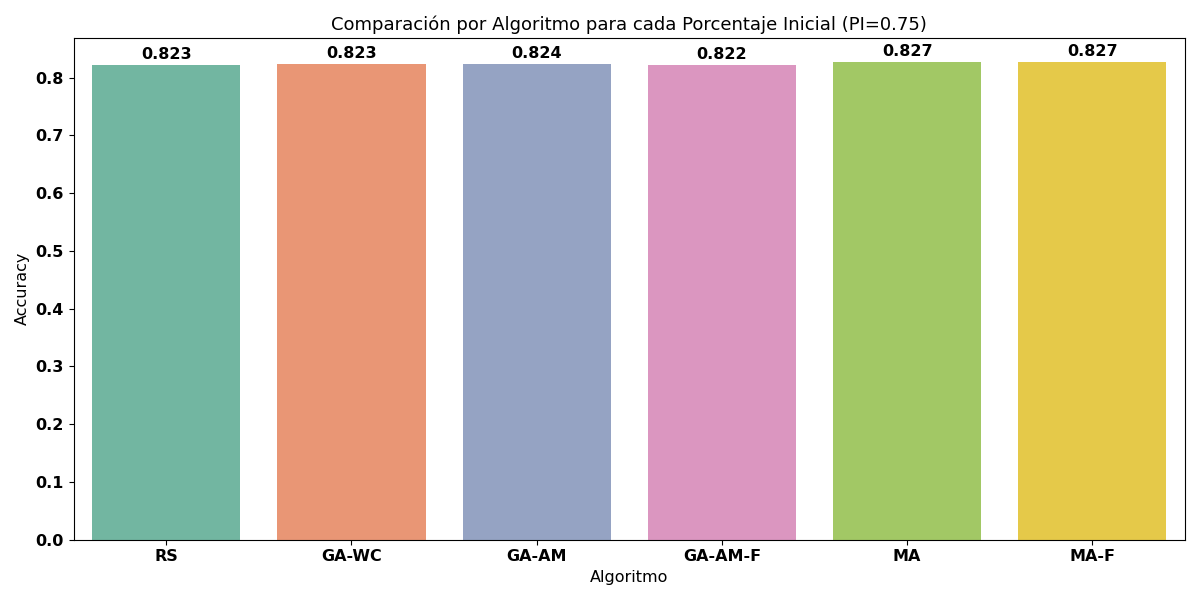
\includegraphics[width=0.7\textwidth]{imagenes/evaluaciones/final/barplot-por-pi/pi-75.png}
    \caption{Comparativa de \textit{accuracy} para cada algoritmo con porcentaje inicial \texttt{75\%}.}
    \label{fig:barplot-por-pi-75}
\end{figure}

\begin{figure}[htp]
    \centering
    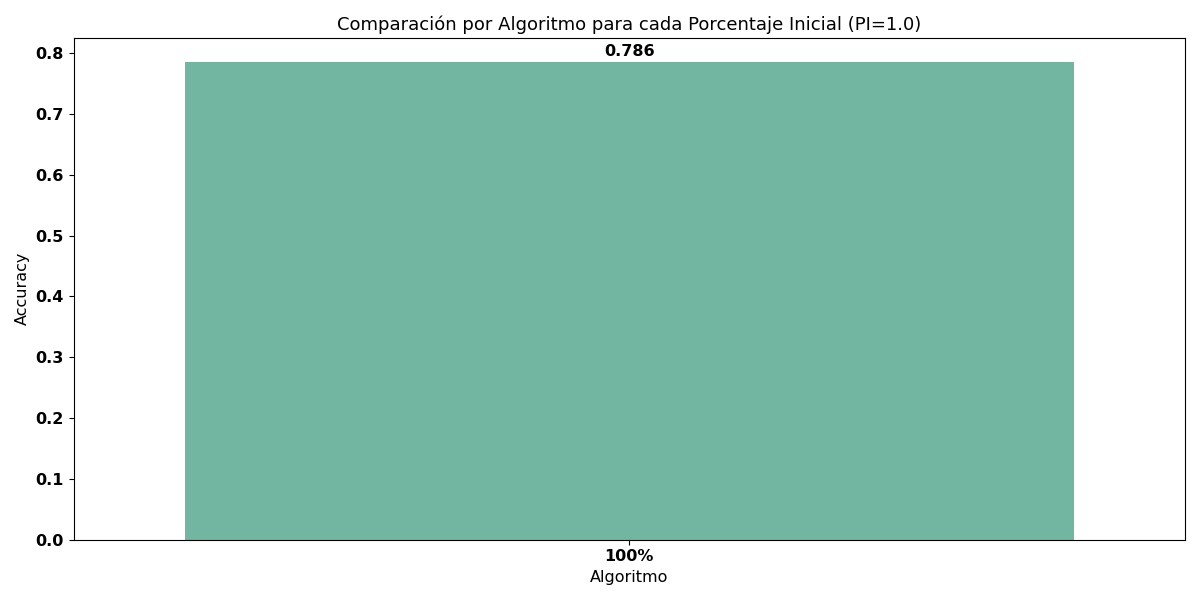
\includegraphics[width=0.7\textwidth]{imagenes/evaluaciones/final/barplot-por-pi/pi-100.png}
    \caption{Comparativa de \textit{accuracy} para cada algoritmo con porcentaje inicial \texttt{100\%}.}
    \label{fig:barplot-por-pi-100}
\end{figure}

En conjunto, este análisis confirma que los algoritmos meméticos, especialmente en su versión libre (\texttt{MA-F}),
representan la mejor alternativa para abordar la selección de subconjuntos de datos en tareas de aprendizaje profundo.
Logran un equilibrio óptimo entre precisión, eficiencia y estabilidad, superando ampliamente a las técnicas basadas en selección aleatoria o enfoques genéticos más sencillos.


\section{Validación con el dataset \texttt{PAINTING}}\label{sec:validacion-con-painting}
Para comprobar la robustez de los algoritmos desarrollados, se validan los experimentos con el dataset \texttt{PAINTING},
caracterizado por una mayor complejidad visual y un número superior de clases respecto al conjunto \texttt{RPS}.
Con el fin de mantener un equilibrio entre complejidad y coste computacional, se limitan los experimentos a los porcentajes iniciales del 25\% y 50\%,
evaluando únicamente los algoritmos más representativos.

En particular, se selecciona el \texttt{MA}, junto con su versión libre, ya que ambos han demostrado ser los más eficaces en las pruebas anteriores.
Para establecer una referencia clara, se incluyen también los resultados obtenidos usando el 100\% del conjunto de datos, y para la comparación de
\textit{accuracy} entre algoritmos también se añade el resultado del \texttt{RS}.

\subsection{Comparación de \textit{accuracy} entre algoritmos}
\begin{figure}[htp]
    \centering
    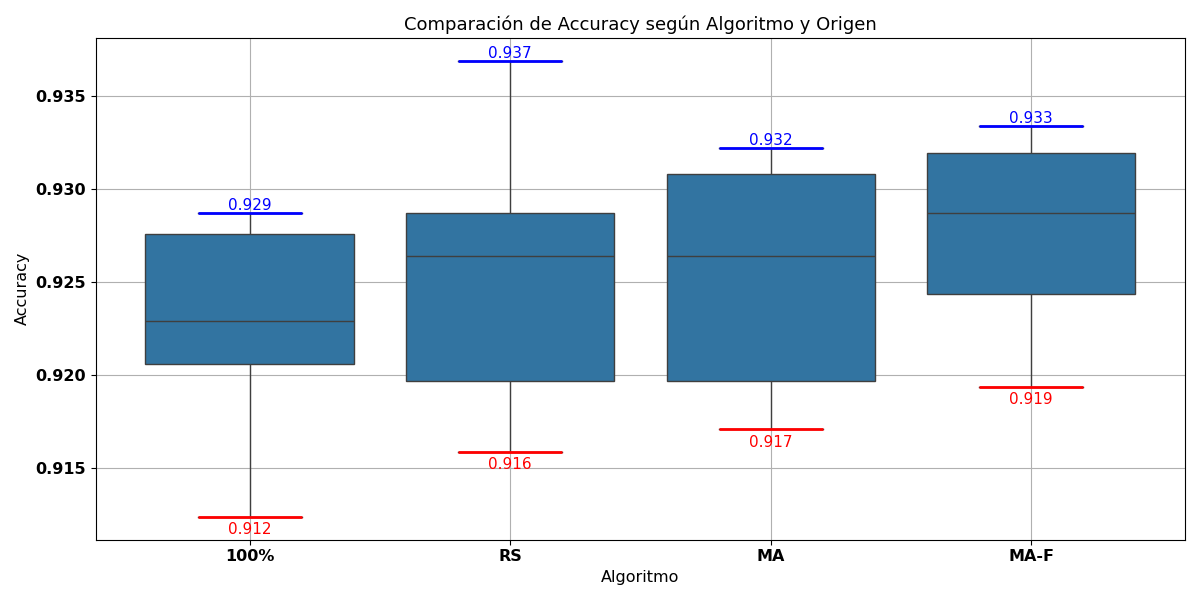
\includegraphics[width=1\textwidth]{imagenes/evaluaciones/painting/comparacion-por-algoritmo.png}
    \caption{Boxplot comparando resultados con el dataset \texttt{PAINTING} usando \textit{accuracy}.}
    \label{fig:comparacion-por-algoritmo}
\end{figure}

En la Figura~\ref{fig:comparacion-por-algoritmo} se comparan los valores de \textit{accuracy} obtenidos al aplicar distintos
algoritmos de selección de subconjuntos en el conjunto de datos \texttt{PAINTING}.
A simple vista, destaca el buen rendimiento de los tres enfoques meméticos frente al uso directo del 100\% del conjunto o la selección aleatoria,
lo cual es especialmente significativo al tratarse de un conjunto con alta complejidad visual y estructural.

El \texttt{MA-F} obtiene el mejor rendimiento general, con una mediana que ronda el \textbf{0.927} y un valor máximo de \textbf{0.933},
superando incluso la ejecución con el 100\% de los datos, cuyo máximo se sitúa en \textbf{0.929}.
Esto no solo refuerza su capacidad de generalización, sino que demuestra que una selección optimizada puede superar a la totalidad del conjunto original,
posiblemente por eliminar ejemplos redundantes o incluso perjudiciales.

El \texttt{MA} también muestra una precisión elevada, con una mediana apenas inferior al libre, y un máximo de \textbf{0.931}.
Sin embargo, su varianza es ligeramente mayor, lo que sugiere que la falta de ajuste dinámico del tamaño del subconjunto puede limitar su adaptabilidad en ciertas ejecuciones.

Por otro lado, la selección aleatoria, aunque muestra valores aceptables, vuelve a confirmar su principal debilidad: la alta dispersión.
Con un mínimo de \textbf{0.916} y una mediana prácticamente idéntica a la obtenida con el uso completo del dataset,
su comportamiento se sitúa como una referencia básica pero poco fiable.
Puede alcanzar buenos resultados, pero lo hace de forma inconsistente y sin mecanismos que garanticen estabilidad.

La ejecución con el \textbf{100\%} de los datos, utilizada como referencia absoluta, queda por debajo de las soluciones obtenidas por los algoritmos meméticos.
Esto valida empíricamente que no es la cantidad de datos, sino su calidad y representatividad, lo que determina la eficacia del entrenamiento en entornos complejos.

En resumen, los algoritmos meméticos, especialmente en su versión libre, muestran el mejor rendimiento en términos de precisión y estabilidad,
superando al uso del 100\% de los datos y al enfoque aleatorio.

\subsection{Impacto del porcentaje inicial}
\begin{figure}[htp]
    \centering
    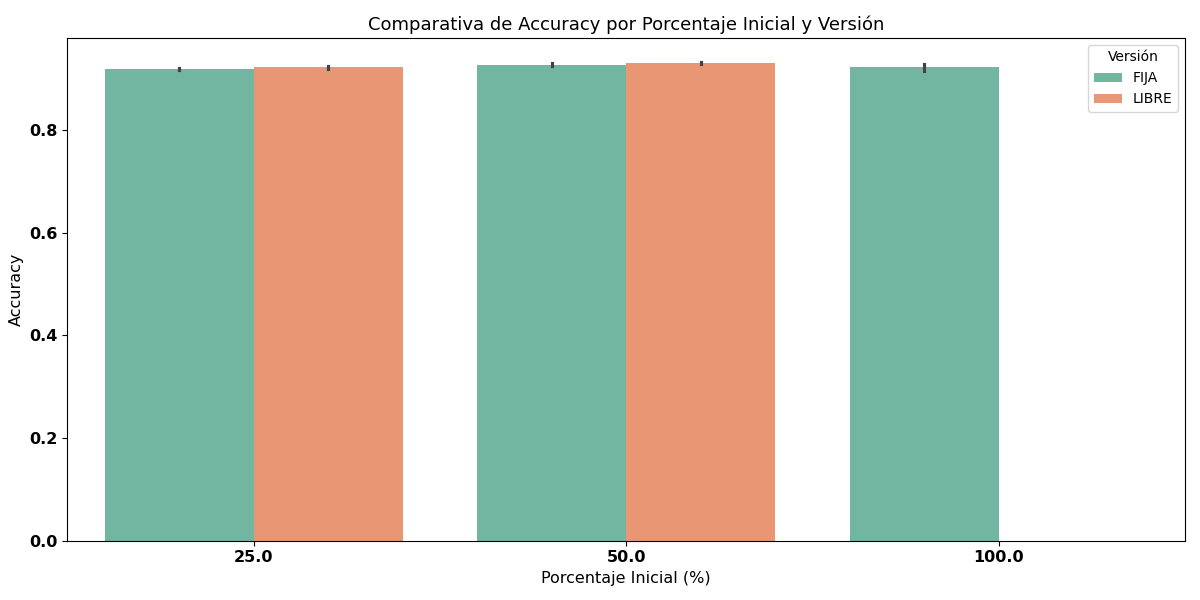
\includegraphics[width=1\textwidth]{imagenes/evaluaciones/painting/comparacion-por-porcentaje.png}
    \caption{Diagrama de barras de \textit{accuracy} según el porcentaje inicial de datos del \texttt{MA}, \texttt{MA-F} y el 100\%.}
    \label{fig:accuracy_porcentaje_painting}
\end{figure}

\begin{figure}[htp]
    \centering
    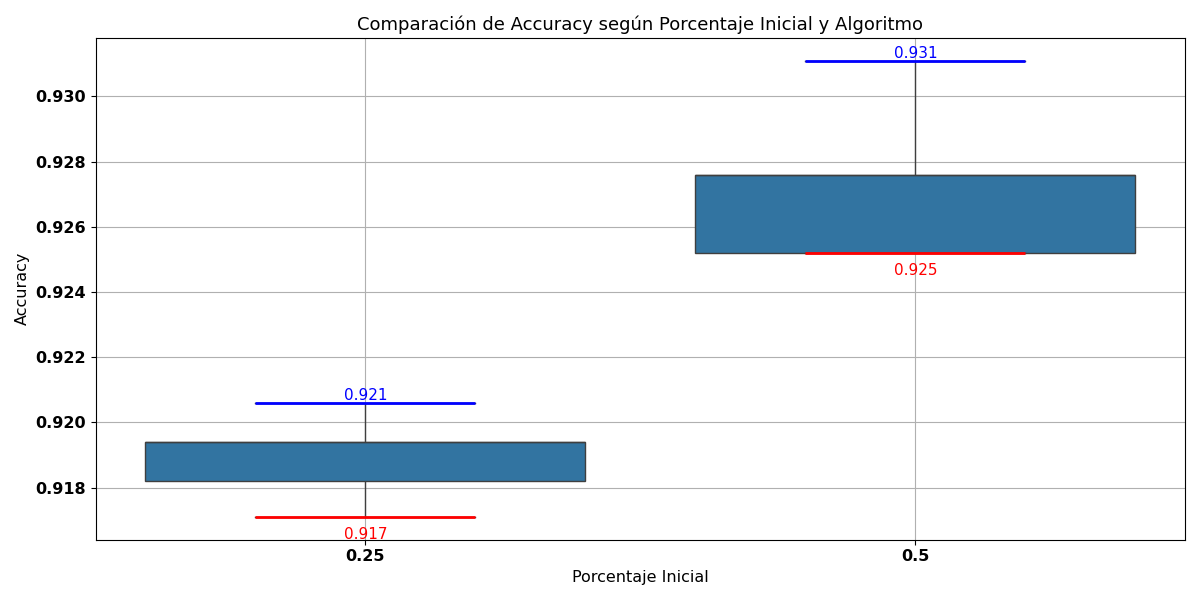
\includegraphics[width=1\textwidth]{imagenes/evaluaciones/painting/comparacion-por-porcentaje-mem.png}
    \caption{Boxplot de \textit{accuracy} para el algoritmo memético (\texttt{MA}) según el porcentaje inicial de datos en el dataset \texttt{PAINTING}.}
    \label{fig:comparacion-por-porcentaje-mem}
\end{figure}

\begin{figure}[htp]
    \centering
    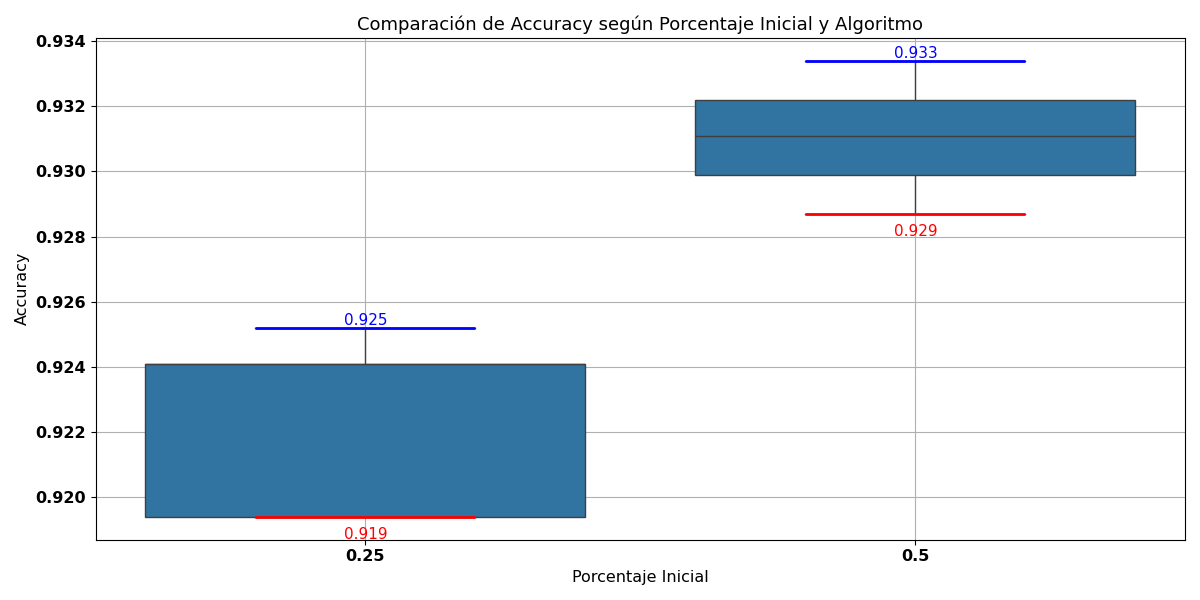
\includegraphics[width=1\textwidth]{imagenes/evaluaciones/painting/comparacion-por-porcentaje-mem-f.png}
    \caption{Boxplot de \textit{accuracy} para el algoritmo memético libre (\texttt{MA-F}) según el porcentaje inicial de datos en el dataset \texttt{PAINTING}.}
    \label{fig:comparacion-por-porcentaje-mem-f}
\end{figure}

\begin{table}[htp]
    \centering
    \resizebox{\textwidth}{!}{
        \begin{tabular}{P{2.5cm} P{2cm} P{2.5cm} P{2.5cm} P{2.5cm} P{2.5cm} P{2cm}}
            \toprule
            \textbf{Algoritmo} & \textbf{Accuracy (Avg)} & \textbf{Precision (Avg)} & \textbf{Recall (Avg)} & \textbf{F1-score (Avg)} & \textbf{Evaluaciones} & \textbf{Porc.
            Final}                                                                                                                                                            \\
            \midrule
            \multicolumn{7}{l}{\textbf{25\%}}                                                                                                                                 \\
            \midrule
            MA                 & 91,89\%                 & 91,63\%                  & 91,89\%               & 91,67\%                 & 100                   & 25,00\%       \\
            MA-F               & 92,24\%                 & 92,06\%                  & 92,24\%               & 92,09\%                 & 100                   & 41,35\%       \\
            \midrule
            \multicolumn{7}{l}{\textbf{50\%}}                                                                                                                                 \\
            \midrule
            MA                 & 92,73\%                 & 92,61\%                  & 92,73\%               & 92,63\%                 & 100                   & 50,00\%       \\
            MA-F               & 93,11\%                 & 93,00\%                  & 93,11\%               & 93,01\%                 & 100                   & 68,69\%       \\
            \midrule
            \multicolumn{7}{l}{\textbf{100\%}}                                                                                                                                \\
            \midrule
            100\%              & 92,24\%                 & 92,05\%                  & 92,24\%               & 92,06\%                 & 1                     & 100,00\%      \\
            \bottomrule
        \end{tabular}
    }
    \caption{Resultados de los algoritmos meméticos y uso del 100\% en el dataset \texttt{PAINTING}.}
    \label{tab:resultados-memetico-painting}
\end{table}

\colorbox{yellow}{FALTA añadir los resultados del 75\%.}


\colorbox{yellow}{FALTA ajustar mejor el analisis.}

La Figura~\ref{fig:accuracy_porcentaje_painting} muestra cómo varía el rendimiento del modelo (medido en términos de \textit{accuracy})
al utilizar diferentes porcentajes iniciales de datos para los algoritmos meméticos en el dataset \texttt{PAINTING}.
Lo primero que destaca es que el uso del 50\% del conjunto original no solo logra un rendimiento equiparable, sino incluso superior al uso del 100\%.
Con una mediana cercana a \textbf{0.930} y un máximo de \textbf{0.933}, este porcentaje logra un equilibrio ideal entre compresión de datos y preservación de información relevante.

Este resultado sugiere que, a partir de cierto umbral, añadir más datos no solo deja de aportar valor, sino que puede introducir ruido o redundancia.
En este caso, el entrenamiento con el 100\% de los datos exhibe mayor dispersión y un mínimo significativamente más bajo (\textbf{0.912}),
lo cual indica una mayor variabilidad entre ejecuciones y una menor estabilidad general.

Por otro lado, el uso del 25\% inicial también demuestra un rendimiento sorprendentemente competitivo,
alcanzando un máximo de \textbf{0.925}.
Sin embargo, su rango intercuartílico más estrecho (menor dispersión de los resultados) y su menor valor mínimo
(\textbf{0.917}) evidencian una cierta fragilidad ante la reducción excesiva:
puede funcionar bien si la selección es óptima, pero el margen de error es menor.

Este comportamiento ilustra un fenómeno interesante en la reducción de datos: no existe una relación lineal entre cantidad de datos y precisión,
sino que el valor está en la calidad y representatividad del subconjunto.
El resultado más robusto refuerza la hipótesis de que existe un punto de saturación
a partir del cual la adición de ejemplos tiene un efecto marginal o incluso contraproducente en modelos convolucionales.

En resumen, los resultados respaldan la viabilidad de utilizar una fracción cuidadosamente seleccionada de datos para obtener
resultados comparables o incluso superiores al uso del conjunto completo.

\subsection{Equilibrio en la distribución de clases}
\begin{figure}[htp]
    \centering
    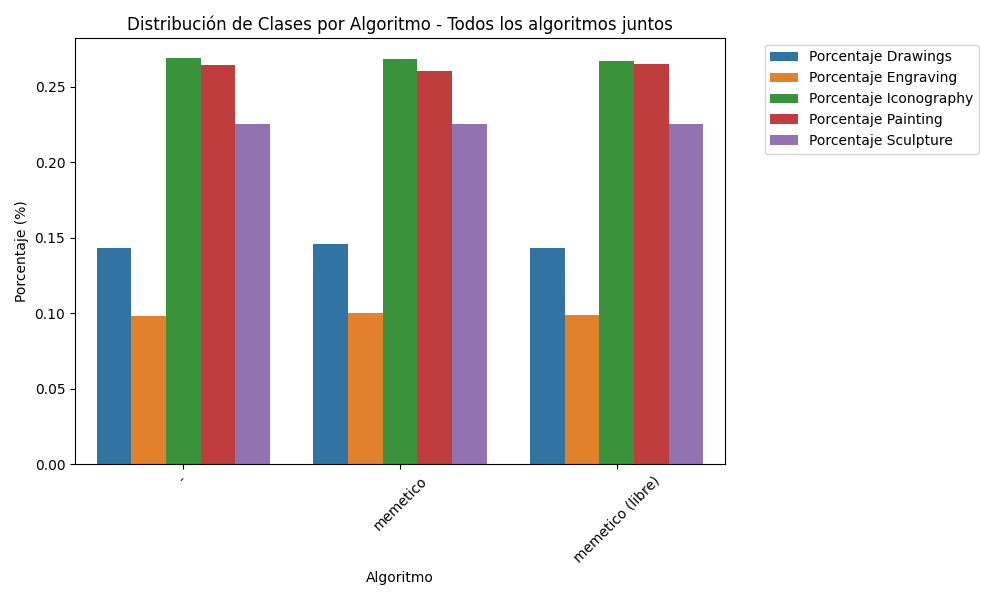
\includegraphics[width=0.9\textwidth]{imagenes/evaluaciones/painting/balance-de-clases-por-algoritmo.png}
    \caption{Distribución de clases seleccionadas por cada algoritmo.}
    \label{fig:balance_clases_painting}
\end{figure}

La Figura~\ref{fig:balance_clases_painting} muestra la proporción de clases preservada por cada algoritmo durante el proceso de reducción.
Se observa que tanto el \texttt{MA} como el \texttt{MA-F} mantienen una distribución prácticamente idéntica a la original,
sin introducir sesgos estructurales.

Las clases mayoritarias (\texttt{Iconography}, \texttt{Painting} y \texttt{Sculpture}) se mantienen consistentes en su proporción,
al igual que las clases minoritarias (\texttt{Drawings} y \texttt{Engraving}).
Esta conservación sugiere que el proceso de selección no actúa de forma aleatoria ni ciega,
sino que incorpora implícitamente una presión hacia la diversidad, lo cual es clave en problemas multiclase.

\subsection{Evolución del tamaño del subconjunto}
\begin{figure}[htp]
    \centering
    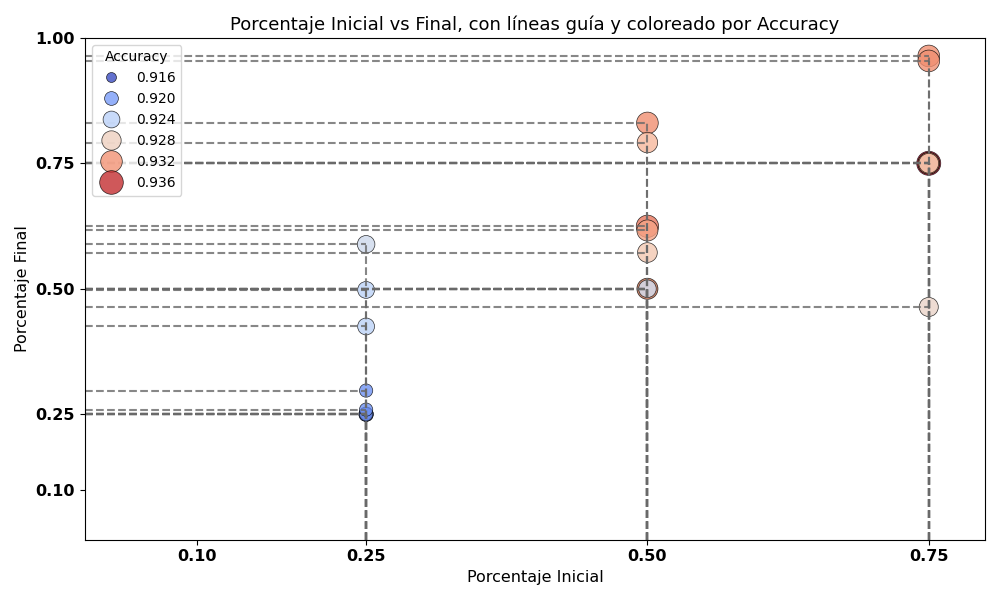
\includegraphics[width=0.9\textwidth]{imagenes/evaluaciones/painting/scatter-por-porcentaje.png}
    \caption{Evolución del tamaño del subconjunto seleccionado por los algoritmos libres según el porcentaje inicial.}
    \label{fig:evolucion_porcentaje_libre}
\end{figure}

\colorbox{yellow}{Volver a mencionar la tabla de resultados.}

En la Figura~\ref{fig:evolucion_porcentaje_libre} se analiza cómo evoluciona el tamaño de los subconjuntos seleccionados por los algoritmos libres respecto al valor inicial.
Se observa que el \texttt{MA-F} tiende a incrementar el porcentaje de imágenes seleccionadas durante el proceso evolutivo.

Este comportamiento adaptativo pone de manifiesto la capacidad del algoritmo para ajustar dinámicamente la escala de la solución en función de la complejidad del problema.
A diferencia de enfoques con tamaño fijo, el algoritmo libre no solo decide qué ejemplos seleccionar, sino también cuántos,
ampliando el conjunto cuando detecta que puede mejorar el rendimiento sin incurrir en sobreajuste.

Además, se observa que al partir del 25\% inicial, el algoritmo tiende a aumentar el tamaño del subconjunto hasta un 16,35\% adicional,
en cambio, al partir del 50\% inicial, el crecimiento es mayor, alcanzando un 18,69\% adicional.
Este hecho puede sugerir una cierta prudencia evolutiva: el algoritmo no se expande indiscriminadamente,
sino que responde a señales de mejora en el proceso de evaluación.
Este mecanismo emergente refuerza la versatilidad del enfoque libre, que no solo busca soluciones de alta calidad,
sino que lo hace optimizando también el volumen de datos utilizados.


\bigskip

\subsection*{Síntesis final de la validación con \texttt{PAINTING}}
Los resultados obtenidos con el dataset \texttt{PAINTING} confirman la solidez y capacidad de generalización de los algoritmos desarrollados.
Tanto el enfoque memético estándar como, especialmente, su versión libre, lograron mantener un rendimiento competitivo en un entorno más complejo y con mayor número de clases.

Se evidencia que es posible superar el rendimiento del conjunto completo de entrenamiento utilizando únicamente un subconjunto bien seleccionado,
reduciendo significativamente el volumen de datos sin comprometer la precisión.
Además, los algoritmos meméticos demuestra preservar el equilibrio entre clases y adaptarse dinámicamente al tamaño del subconjunto,
lo que constituye una ventaja clave en tareas reales donde no siempre se dispone de datasets perfectamente balanceados ni completos.

En conjunto, esta validación externa no solo refuerza las conclusiones obtenidas con \texttt{RPS},
sino que demuestra que el uso de técnicas evolutivas, y en particular las variantes libres, puede ser una alternativa eficaz,
escalable y controlable frente a la selección masiva o aleatoria de datos en procesos de entrenamiento profundo.

% !TeX root = ../proyecto.tex

\chapter{Conclusiones}\label{ch:conclusiones}
Este Trabajo de Fin de Grado aborda el problema de la reducción de conjuntos de datos en el contexto del aprendizaje profundo,
proponiendo el uso de algoritmos meméticos como técnica de selección de instancias.
A lo largo del desarrollo se diseñan, implementan y evalúan diferentes enfoques evolutivos (genéticos y meméticos),
con el objetivo de identificar subconjuntos representativos de imágenes que permitan entrenar modelos convolucionales de forma eficiente y sin pérdida significativa de rendimiento.

El estudio se centra en evaluar cómo diferentes variantes algorítmicas impactan sobre la precisión, la estabilidad y el tamaño final del conjunto de entrenamiento.
Para ello, se utilizan dos modelos de referencia ampliamente extendidos (\texttt{ResNet50} y \texttt{MobileNetV2}) y tres conjuntos de datos con distintos niveles de complejidad: `\texttt{Rock, Paper, Scissors}', `\texttt{PAINTING}' y `\texttt{CIFAR-10}'.

Los resultados experimentales permiten extraer varias conclusiones clave:

\begin{itemize}
      \item El uso de algoritmos evolutivos mejora notablemente la calidad de los subconjuntos generados en comparación con estrategias aleatorias o deterministas.
            Incluso las versiones básicas, como el algoritmo genético clásico, superan con claridad al enfoque aleatorio.

      \item Las mejoras introducidas en los operadores de cruce y mutación (ponderación basada en fitness y mutación adaptativa)
            incrementan la estabilidad y precisión de los resultados, especialmente en escenarios con porcentajes bajos de datos iniciales.

      \item La inclusión del reinicio poblacional ofrece cierto beneficio en términos de diversidad,
            aunque no aporta mejoras significativas respecto a las versiones mejoradas del genético en cuanto a precisión media.

      \item Las versiones \textit{libres} de los algoritmos, donde el tamaño del subconjunto se ajusta dinámicamente,
            permiten alcanzar un equilibrio más eficaz entre precisión y tamaño final.
            Este enfoque demuestra ser especialmente útil cuando no se conoce a priori la porcentaje óptima de datos para entrenar.

      \item El algoritmo memético, y en particular su versión libre (MA-F), alcanza los mejores resultados globales.
            Este enfoque logra una elevada precisión, una notable reducción del conjunto de datos y una gran estabilidad entre ejecuciones,
            consolidándose como la solución más eficaz del estudio.
\end{itemize}


La validación con un segundo conjunto de datos (`\texttt{PAINTING}'), más complejo y con mayor número de clases, y con un tercer conjunto (`\texttt{CIFAR-10}'),
considerablemente más exigente por su variabilidad intraclase y baja resolución, permite comprobar la capacidad de generalización de los enfoques propuestos.
El algoritmo memético libre no solo mantiene su rendimiento, sino que en algunos casos supera a la precisión obtenida con el 100\% del conjunto completo.
Además, se confirma que las soluciones generadas preservan una distribución equilibrada de clases y ajustan el tamaño del subconjunto según la dificultad del problema.


Los resultados obtenidos tienen implicaciones prácticas significativas.
Queda demostrado que es posible reducir de forma significativa los conjuntos de datos para entrenar modelos convolucionales sin comprometer el rendimiento,
siempre que se utilicen estrategias de selección guiadas y adaptativas.
Aunque la selección de instancias conlleva un coste computacional adicional durante su ejecución, 
este esfuerzo inicial se justifica al permitir una notable reducción en el tiempo de entrenamiento e inferencia de los modelos explorados.
Además, facilita la auditoría y trazabilidad de los datos, aspectos fundamentales en entornos donde estas exigencias normativas son prioritarias.
A medio plazo, el uso de subconjuntos optimizados puede reducir el coste global cuando se entrenan múltiples modelos o configuraciones diferentes.

Como líneas futuras, se plantea:
\begin{itemize}
      \item Aplicar las técnicas propuestas en tareas más complejas, como la segmentación semántica o la clasificación multietiqueta,
            donde la reducción del conjunto de datos puede tener un impacto aún más relevante.
      \item Incorporar múltiples objetivos en el proceso de selección, convirtiéndolo en un problema de optimización multiobjetivo.
            Por ejemplo, se podría considerar aspectos como el tiempo de entrenamiento, el coste computacional total o la eficiencia en la fase de inferencia,
            además de las métricas clásicas de rendimiento.
      \item Explorar la integración de los algoritmos meméticos con otras estrategias de reducción de datos, como la destilación de conocimiento o la poda de redes neuronales,
            con el objetivo de combinar distintas aproximaciones complementarias.
\end{itemize}

En resumen, los hallazgos de este estudio ponen de manifiesto el potencial de los algoritmos meméticos en la reducción eficiente de conjuntos de datos para aprendizaje profundo.
Este trabajo demuestra que la combinación de técnicas evolutivas y búsqueda local, aplicada de forma flexible y adaptativa,
constituye una herramienta poderosa para optimizar el entrenamiento de modelos de aprendizaje profundo.
Más allá de la mejora en precisión o eficiencia, esta línea de investigación apunta hacia un aprendizaje más sostenible, trazable y accesible,
en línea con las necesidades actuales de la inteligencia artificial moderna.

Desde un punto de vista personal, este proyecto ha representado un desafío enriquecedor tanto a nivel técnico como organizativo.
La implementación completa de los algoritmos, la gestión eficiente del entorno experimental y
la interpretación rigurosa de los resultados me han permitido consolidar conocimientos clave en aprendizaje automático y optimización.
Asimismo, la dificultad de compaginar este trabajo con responsabilidades laborales ha reforzado mi compromiso con el rigor y la constancia,
valores que considero fundamentales en mi futuro profesional.

% Bibliografía y apéndices
\chapter{Bibliografía}\label{ch:bibliografia}
\printbibliography[heading=none, category=cited]

% \chapter{Bibliografía de Referencia\texorpdfstring{\protect\footnotemark}{}}%
% \footnotetext{Este capítulo contiene las referencias bibliográficas consultadas (que no han sido citadas en el cuerpo del documento).}
% \printbibliography[heading=none, notcategory=cited]


%\appendix
%\input{apendices/manual_usuario/manual_usuario}
%\input{glosario/entradas_glosario}

\chapter*{}
\thispagestyle{empty}

\end{document}
% !TEX root = proyecto.tex
